\documentclass[a4paper]{book}

\usepackage[left=3.81cm, right=2.54cm, top=2.54cm, bottom=3.17cm]{geometry}
\usepackage[T1]{fontenc} 
%\usepackage[spanish, activeacute]{babel}
%\usepackage[latin1]{inputenc} %Letras con acentos, enies.

%\usepackage{amssymb}
%\usepackage{amsmath}
%\usepackage{amsthm} % theorems
\usepackage{enumerate}
\usepackage{epsfig}
\usepackage{multirow}

\usepackage{graphicx}
\usepackage{tikz}
\usetikzlibrary{shapes,arrows,automata,positioning,fit}

\usepackage{url}
\usepackage{verbatim}
\usepackage{array}

\usepackage{algorithmic}

\usepackage{fixme}
\usepackage{xspace}
\usepackage{ifthen}

\usepackage{pdfpages}

\renewcommand{\listtablename}{Indice de Tablas}
\renewcommand{\tablename}{Tabla}

% Sin sangria
%\parindent=0mm  

% Espacio entre parrafos
%\parskip=4mm

% Dialogue template
\newenvironment{dialogue}%
   {\begin{it}%
    \begin{list}{}%
         {\setlength{\leftmargin}{.3cm}}%
         \item[]}%
   {\end{list}%
    \end{it}}

\usetikzlibrary{automata}
\usepackage{floatrow}
\DeclareFloatFont{tiny}{\tiny}% "scriptsize" is defined by floatrow, "tiny" not
\floatsetup[table]{font=tiny}
\usepackage{algorithm}

\newcommand{\tup}[1]{\langle #1 \rangle}
\newcommand{\puse}{\ensuremath{\textsf{p}_\textit{use}}}
\newcommand{\randomuse}{\ensuremath{\textsf{rnd}_\emph{use}}\xspace}
\newcommand{\incuse}{\ensuremath{\textsf{inc}_\emph{use}}\xspace}
\newcommand{\RE}{\textsf{RE}\xspace}
\newcommand{\REL}{\textsf{REL}\xspace}
\newcommand{\IR}{\textrm{I}\!\textrm{R}}
\newcommand{\gM}{\mathcal{M}}
\newcommand{\el}{\ensuremath{\mathcal{EL}}\xspace}
\newcommand{\interp}[1]{|\!|#1|\!|}


\newcommand{\nBlue}{\textsf{blue}\xspace}
\newcommand{\nGreen}{\textsf{green}\xspace}
\newcommand{\nSmall}{\textsf{small}\xspace}
\newcommand{\nBig}{\textsf{big}\xspace}
\newcommand{\nRed}{\textsf{red}\xspace}
\newcommand{\nYellow}{\textsf{yellow}\xspace}
\newcommand{\nBall}{\textsf{ball}\xspace}
\newcommand{\nCube}{\textsf{cube}\xspace}
\newcommand{\nOntop}{\textsf{ontop}\xspace}
\newcommand{\nTop}{\textsf{top}\xspace}
\newcommand{\nBelow}{\textsf{below}\xspace}
\newcommand{\nRightof}{\textsf{rightof}\xspace}
\newcommand{\nLeftof}{\textsf{leftof}\xspace}
\newcommand{\nLeft}{\textsf{left}\xspace}




\begin{document}

% PARTE PRELIMINAR
%\frontmatter % Numeros de paginas con numeros romanos

\thispagestyle{empty}

\begin{titlepage}
\begin{center}

{ \vspace*{1cm} }
\huge{\textsc{\textmd{Universidad Nacional de C\'ordoba}}}\\[1cm]
\Large{\textsc{\textmd{Facultad de Matem\'atica, Astronom\'ia y F\'isica}}}\\[1cm]

\includegraphics[scale=0.1]{preliminar/unc}\\[1.3cm]

\Large{Trabajo final del Doctorado en Ciencias de la Computaci\'on}\\[1cm]

\LARGE{\textbf{Generaci\'on de expresiones referenciales: el punto de vista l\'ogico, el m\'as humano }}\\[2cm]

\Large{Alumna: Ivana Romina Altamirano}\\[1.3cm]

\Large{Supervisora: Luciana Benotti}

\vfill
\vfill
%\large{C\'ORDOBA} \hfill \large{ARGENTINA}\\[2cm]

\large{C\'ORDOBA } \large{ARGENTINA}\\ 
\large{Diciembre, 2013}


\end{center}
\end{titlepage}

%{ \vspace*{1cm} }

\Large{\textsc{P\'agina para los evaluadores}}\\[3cm]

\large{Calificaci\'on:}\\[1.8cm]

\large{Comentarios:}\\[5cm]

\begin{center}
........................................ \qquad\qquad\qquad\qquad ........................................\\[3.5cm]
........................................\\
\end{center}

\vfill

\begin{flushright}
......................................................\\
\large{Lugar para la fecha de Evaluaci\'on}
\end{flushright}


\newpage
\mbox{}
% dedicatoria.tex
% Dedicatoria de la tesis

\vspace*{\fill}

%\begin{flushright}
%    \emph{Gracias Lu, Carlos \ldots}
%\end{flushright}

Le dedico esta tesis a cada persona a quien le robe alg\'un minuto para realizarla. A Luciana Benotti, mi directora y amiga, que sin duda fue la que m\'as le dedic\'o tiempo a mi tesis, que estuvo a mi lado gu\'iandome y consiguiendo nuevos desaf\'ios para m\'i, a cada instante. A Carlos Areces por ayudarnos con el marco te\'orico. A mi hija que supo esperar el momento adecuado para llegar al mundo, y darme un recreo en la tesis. A Boris, a mi familia. 


\vspace{\fill}

\newpage
\mbox{}
\thispagestyle{empty}

\begin{itemize}
	\item \textbf{\textsc{Clasificaci�n de Biblioteca:}} \\ \\  \\ \\

	\item \textbf{\emph{\textsc{Palabras Clave:} \\ expresiones referenciales, aprendizaje autom�tico, bisimulaci�n, evaluaci�n.}}
\end{itemize}

\begin{center}

{ \vspace*{1cm} }
\huge{\textbf{\textsc{\textmd{Resumen}}}}\\[1cm]
%\Large{\textsc{\textmd{Facultad de Matem�tica, Astronom\'ia y F\'isica}}}\\[1cm]

\end{center}

\normalsize{

La Generaci\'on de Expresiones Referenciales es una sub-\'area de la generaci\'on de lenguaje natural, es un \'area que ha sido muy estudiada, sin embargo la mayor\'ia de las investigaciones se centraron en generar expresiones de menor longitud, no compar\'andolas con las que hab\'ia en corpus. Las pocas excepciones que tuvieron esto en cuenta, usan una lista ordenada de los atributos e incluyen propiedades en el orden de la lista, esta lista es fija, otra cosa que no se tuvo en cuenta es que las personas son no-deterministas cuando se refieren a cosas, en esta tesis se propone un algoritmo para la generaci�n de expresiones referenciales (ERs) que adapta la aproximaci�n 
de~\cite{arec2:2008:Areces,arec:usin11} para que sea no-determin\'istico, incluya sobre-especificaci�n y probabilidades de uso de las palabras aprendidas a partir de corpus. Luego de introducir el algoritmo discutimos como las probabilidades requeridas pueden ser computadas para cualquier dominio para el cual existe un corpus de ERs y como las probabilidades pueden ser ajustadas para nuevas escenas en el dominio usando aprendizaje autom�tico. Ejemplificamos como computar las probabilidades sobre el corpus GRE3D7 de \cite{viet:gene11} y el TUNA corpus de \cite{gatt-balz-kow:2008:ENLG}. El algoritmo resultante es capaz de generar diferentes expresiones referenciales para el mismo target con una frecuencia similar a aquella observada en el corpus. Evaluamos emp�ricamente el nuevo algoritmo sobre el corpus GR3D7, y mostramos que la distribuci�n de probabilidad de las expresiones referenciales generadas por el algoritmo machean las encontradas en el corpus con alta precisi�n. Tambi�n comparamos nuestros resultados con los resultados the \cite{graph08}, los ganadores de la competencia NLG Challenge sobre selecci�n de atributos para generaci�n de expresiones referenciales (ASGRE). Proveemos un an�lisis de error y conclusiones para ambos corpus. Se cre� un nuevo corpus de ER sobre el cual se describe y se dan los resultados obtenidos, este nuevo corpus realizado sobre un entorno mucho m�s natural nos d� la certeza de que nuestro algoritmo se puede aplicar a sistemas de la vida real.
}

\begin{center}

{ \vspace*{1cm} }
\huge{\textbf{\textsc{\textmd{Abstract}}}}\\[1cm]
%\Large{\textsc{\textmd{Facultad de Matem�tica, Astronom\'ia y F\'isica}}}\\[1cm]

\end{center}

\normalsize{
We propose an algorithm for the generation of referring expressions (REs) that adapts the approach of~\cite{arec2:2008:Areces,arec:usin11} 
to include overspecification and probabilities learned from corpora.  After introducing the algorithm, we discuss how probabilities required as 
input can be computed for any given domain for which a suitable corpus of REs is available, and how the probabilities can be adjusted for new scenes in the domain using a machine learning approach.  
We exemplify how to compute probabilities over the GRE3D7 corpus of~\cite{viet:gene11} \textit{and the TUNA corpus of ~\cite{gatt-balz-kow:2008:ENLG}}.
The resulting algorithm is able to generate different referring expressions for the same target with a frequency similar to that observed in corpora. 
%Moreover, the most frequently generated referring expressions not in the corpus are also semantically natural, indicating that the algorithm 
%can generalize from the learning data. \\
We empirically evaluate the new algorithm over the GRE3D7 corpus, and show that the probability distribution of the generated referring expressions 
matches the one found in the corpus with high accuracy. We also compare our results with the results of~\cite{graph08} the winners of the NLG Challenge on Attribute Selection for Generating Referring Expressions (ASGRE). We provide error analysis and conclusion for both corpus. 
In this thesis we create a new corpora or REs but the new corpora is much more natural, the REs create by the algorithm for this new corpora are shown with those results we can say that our algorithm is usefull in systems of the real life.





\tableofcontents
%\include{prefacio} --- Esto es opcional, no es necesario
%\include{agradecimientos} Esto se hace al final
%\thispagestyle{empty}

\begin{itemize}
	\item \textbf{\textsc{Clasificaci�n de Biblioteca:}} \\ \\  \\ \\

	\item \textbf{\emph{\textsc{Palabras Clave:} \\ expresiones referenciales, aprendizaje autom�tico, bisimulaci�n, evaluaci�n.}}
\end{itemize}

\begin{center}

{ \vspace*{1cm} }
\huge{\textbf{\textsc{\textmd{Resumen}}}}\\[1cm]
%\Large{\textsc{\textmd{Facultad de Matem�tica, Astronom\'ia y F\'isica}}}\\[1cm]

\end{center}

\normalsize{

La Generaci\'on de Expresiones Referenciales es una sub-\'area de la generaci\'on de lenguaje natural, es un \'area que ha sido muy estudiada, sin embargo la mayor\'ia de las investigaciones se centraron en generar expresiones de menor longitud, no compar\'andolas con las que hab\'ia en corpus. Las pocas excepciones que tuvieron esto en cuenta, usan una lista ordenada de los atributos e incluyen propiedades en el orden de la lista, esta lista es fija, otra cosa que no se tuvo en cuenta es que las personas son no-deterministas cuando se refieren a cosas, en esta tesis se propone un algoritmo para la generaci�n de expresiones referenciales (ERs) que adapta la aproximaci�n 
de~\cite{arec2:2008:Areces,arec:usin11} para que sea no-determin\'istico, incluya sobre-especificaci�n y probabilidades de uso de las palabras aprendidas a partir de corpus. Luego de introducir el algoritmo discutimos como las probabilidades requeridas pueden ser computadas para cualquier dominio para el cual existe un corpus de ERs y como las probabilidades pueden ser ajustadas para nuevas escenas en el dominio usando aprendizaje autom�tico. Ejemplificamos como computar las probabilidades sobre el corpus GRE3D7 de \cite{viet:gene11} y el TUNA corpus de \cite{gatt-balz-kow:2008:ENLG}. El algoritmo resultante es capaz de generar diferentes expresiones referenciales para el mismo target con una frecuencia similar a aquella observada en el corpus. Evaluamos emp�ricamente el nuevo algoritmo sobre el corpus GR3D7, y mostramos que la distribuci�n de probabilidad de las expresiones referenciales generadas por el algoritmo machean las encontradas en el corpus con alta precisi�n. Tambi�n comparamos nuestros resultados con los resultados the \cite{graph08}, los ganadores de la competencia NLG Challenge sobre selecci�n de atributos para generaci�n de expresiones referenciales (ASGRE). Proveemos un an�lisis de error y conclusiones para ambos corpus. Se cre� un nuevo corpus de ER sobre el cual se describe y se dan los resultados obtenidos, este nuevo corpus realizado sobre un entorno mucho m�s natural nos d� la certeza de que nuestro algoritmo se puede aplicar a sistemas de la vida real.
}

\begin{center}

{ \vspace*{1cm} }
\huge{\textbf{\textsc{\textmd{Abstract}}}}\\[1cm]
%\Large{\textsc{\textmd{Facultad de Matem�tica, Astronom\'ia y F\'isica}}}\\[1cm]

\end{center}

\normalsize{
We propose an algorithm for the generation of referring expressions (REs) that adapts the approach of~\cite{arec2:2008:Areces,arec:usin11} 
to include overspecification and probabilities learned from corpora.  After introducing the algorithm, we discuss how probabilities required as 
input can be computed for any given domain for which a suitable corpus of REs is available, and how the probabilities can be adjusted for new scenes in the domain using a machine learning approach.  
We exemplify how to compute probabilities over the GRE3D7 corpus of~\cite{viet:gene11} \textit{and the TUNA corpus of ~\cite{gatt-balz-kow:2008:ENLG}}.
The resulting algorithm is able to generate different referring expressions for the same target with a frequency similar to that observed in corpora. 
%Moreover, the most frequently generated referring expressions not in the corpus are also semantically natural, indicating that the algorithm 
%can generalize from the learning data. \\
We empirically evaluate the new algorithm over the GRE3D7 corpus, and show that the probability distribution of the generated referring expressions 
matches the one found in the corpus with high accuracy. We also compare our results with the results of~\cite{graph08} the winners of the NLG Challenge on Attribute Selection for Generating Referring Expressions (ASGRE). We provide error analysis and conclusion for both corpus. 
In this thesis we create a new corpora or REs but the new corpora is much more natural, the REs create by the algorithm for this new corpora are shown with those results we can say that our algorithm is usefull in systems of the real life.



 Esto se hace al final



\frontmatter % Numeros de paginas con numeros romanos

\thispagestyle{empty}

\begin{titlepage}
\begin{center}

{ \vspace*{1cm} }
\huge{\textsc{\textmd{Universidad Nacional de C\'ordoba}}}\\[1cm]
\Large{\textsc{\textmd{Facultad de Matem\'atica, Astronom\'ia y F\'isica}}}\\[1cm]

\includegraphics[scale=0.1]{preliminar/unc}\\[1.3cm]

\Large{Trabajo final del Doctorado en Ciencias de la Computaci\'on}\\[1cm]

\LARGE{\textbf{Generaci\'on de expresiones referenciales: el punto de vista l\'ogico, el m\'as humano }}\\[2cm]

\Large{Alumna: Ivana Romina Altamirano}\\[1.3cm]

\Large{Supervisora: Luciana Benotti}

\vfill
\vfill
%\large{C\'ORDOBA} \hfill \large{ARGENTINA}\\[2cm]

\large{C\'ORDOBA } \large{ARGENTINA}\\ 
\large{Diciembre, 2013}


\end{center}
\end{titlepage}

%{ \vspace*{1cm} }

\Large{\textsc{P\'agina para los evaluadores}}\\[3cm]

\large{Calificaci\'on:}\\[1.8cm]

\large{Comentarios:}\\[5cm]

\begin{center}
........................................ \qquad\qquad\qquad\qquad ........................................\\[3.5cm]
........................................\\
\end{center}

\vfill

\begin{flushright}
......................................................\\
\large{Lugar para la fecha de Evaluaci\'on}
\end{flushright}


\newpage
\mbox{}
% dedicatoria.tex
% Dedicatoria de la tesis

\vspace*{\fill}

%\begin{flushright}
%    \emph{Gracias Lu, Carlos \ldots}
%\end{flushright}

Le dedico esta tesis a cada persona a quien le robe alg\'un minuto para realizarla. A Luciana Benotti, mi directora y amiga, que sin duda fue la que m\'as le dedic\'o tiempo a mi tesis, que estuvo a mi lado gu\'iandome y consiguiendo nuevos desaf\'ios para m\'i, a cada instante. A Carlos Areces por ayudarnos con el marco te\'orico. A mi hija que supo esperar el momento adecuado para llegar al mundo, y darme un recreo en la tesis. A Boris, a mi familia. 


\vspace{\fill}

\newpage
\mbox{}
\thispagestyle{empty}

\begin{itemize}
	\item \textbf{\textsc{Clasificaci�n de Biblioteca:}} \\ \\  \\ \\

	\item \textbf{\emph{\textsc{Palabras Clave:} \\ expresiones referenciales, aprendizaje autom�tico, bisimulaci�n, evaluaci�n.}}
\end{itemize}

\begin{center}

{ \vspace*{1cm} }
\huge{\textbf{\textsc{\textmd{Resumen}}}}\\[1cm]
%\Large{\textsc{\textmd{Facultad de Matem�tica, Astronom\'ia y F\'isica}}}\\[1cm]

\end{center}

\normalsize{

La Generaci\'on de Expresiones Referenciales es una sub-\'area de la generaci\'on de lenguaje natural, es un \'area que ha sido muy estudiada, sin embargo la mayor\'ia de las investigaciones se centraron en generar expresiones de menor longitud, no compar\'andolas con las que hab\'ia en corpus. Las pocas excepciones que tuvieron esto en cuenta, usan una lista ordenada de los atributos e incluyen propiedades en el orden de la lista, esta lista es fija, otra cosa que no se tuvo en cuenta es que las personas son no-deterministas cuando se refieren a cosas, en esta tesis se propone un algoritmo para la generaci�n de expresiones referenciales (ERs) que adapta la aproximaci�n 
de~\cite{arec2:2008:Areces,arec:usin11} para que sea no-determin\'istico, incluya sobre-especificaci�n y probabilidades de uso de las palabras aprendidas a partir de corpus. Luego de introducir el algoritmo discutimos como las probabilidades requeridas pueden ser computadas para cualquier dominio para el cual existe un corpus de ERs y como las probabilidades pueden ser ajustadas para nuevas escenas en el dominio usando aprendizaje autom�tico. Ejemplificamos como computar las probabilidades sobre el corpus GRE3D7 de \cite{viet:gene11} y el TUNA corpus de \cite{gatt-balz-kow:2008:ENLG}. El algoritmo resultante es capaz de generar diferentes expresiones referenciales para el mismo target con una frecuencia similar a aquella observada en el corpus. Evaluamos emp�ricamente el nuevo algoritmo sobre el corpus GR3D7, y mostramos que la distribuci�n de probabilidad de las expresiones referenciales generadas por el algoritmo machean las encontradas en el corpus con alta precisi�n. Tambi�n comparamos nuestros resultados con los resultados the \cite{graph08}, los ganadores de la competencia NLG Challenge sobre selecci�n de atributos para generaci�n de expresiones referenciales (ASGRE). Proveemos un an�lisis de error y conclusiones para ambos corpus. Se cre� un nuevo corpus de ER sobre el cual se describe y se dan los resultados obtenidos, este nuevo corpus realizado sobre un entorno mucho m�s natural nos d� la certeza de que nuestro algoritmo se puede aplicar a sistemas de la vida real.
}

\begin{center}

{ \vspace*{1cm} }
\huge{\textbf{\textsc{\textmd{Abstract}}}}\\[1cm]
%\Large{\textsc{\textmd{Facultad de Matem�tica, Astronom\'ia y F\'isica}}}\\[1cm]

\end{center}

\normalsize{
We propose an algorithm for the generation of referring expressions (REs) that adapts the approach of~\cite{arec2:2008:Areces,arec:usin11} 
to include overspecification and probabilities learned from corpora.  After introducing the algorithm, we discuss how probabilities required as 
input can be computed for any given domain for which a suitable corpus of REs is available, and how the probabilities can be adjusted for new scenes in the domain using a machine learning approach.  
We exemplify how to compute probabilities over the GRE3D7 corpus of~\cite{viet:gene11} \textit{and the TUNA corpus of ~\cite{gatt-balz-kow:2008:ENLG}}.
The resulting algorithm is able to generate different referring expressions for the same target with a frequency similar to that observed in corpora. 
%Moreover, the most frequently generated referring expressions not in the corpus are also semantically natural, indicating that the algorithm 
%can generalize from the learning data. \\
We empirically evaluate the new algorithm over the GRE3D7 corpus, and show that the probability distribution of the generated referring expressions 
matches the one found in the corpus with high accuracy. We also compare our results with the results of~\cite{graph08} the winners of the NLG Challenge on Attribute Selection for Generating Referring Expressions (ASGRE). We provide error analysis and conclusion for both corpus. 
In this thesis we create a new corpora or REs but the new corpora is much more natural, the REs create by the algorithm for this new corpora are shown with those results we can say that our algorithm is usefull in systems of the real life.





\tableofcontents
%\include{prefacio} --- Esto es opcional, no es necesario
%\include{agradecimientos} Esto se hace al final
%\thispagestyle{empty}

\begin{itemize}
	\item \textbf{\textsc{Clasificaci�n de Biblioteca:}} \\ \\  \\ \\

	\item \textbf{\emph{\textsc{Palabras Clave:} \\ expresiones referenciales, aprendizaje autom�tico, bisimulaci�n, evaluaci�n.}}
\end{itemize}

\begin{center}

{ \vspace*{1cm} }
\huge{\textbf{\textsc{\textmd{Resumen}}}}\\[1cm]
%\Large{\textsc{\textmd{Facultad de Matem�tica, Astronom\'ia y F\'isica}}}\\[1cm]

\end{center}

\normalsize{

La Generaci\'on de Expresiones Referenciales es una sub-\'area de la generaci\'on de lenguaje natural, es un \'area que ha sido muy estudiada, sin embargo la mayor\'ia de las investigaciones se centraron en generar expresiones de menor longitud, no compar\'andolas con las que hab\'ia en corpus. Las pocas excepciones que tuvieron esto en cuenta, usan una lista ordenada de los atributos e incluyen propiedades en el orden de la lista, esta lista es fija, otra cosa que no se tuvo en cuenta es que las personas son no-deterministas cuando se refieren a cosas, en esta tesis se propone un algoritmo para la generaci�n de expresiones referenciales (ERs) que adapta la aproximaci�n 
de~\cite{arec2:2008:Areces,arec:usin11} para que sea no-determin\'istico, incluya sobre-especificaci�n y probabilidades de uso de las palabras aprendidas a partir de corpus. Luego de introducir el algoritmo discutimos como las probabilidades requeridas pueden ser computadas para cualquier dominio para el cual existe un corpus de ERs y como las probabilidades pueden ser ajustadas para nuevas escenas en el dominio usando aprendizaje autom�tico. Ejemplificamos como computar las probabilidades sobre el corpus GRE3D7 de \cite{viet:gene11} y el TUNA corpus de \cite{gatt-balz-kow:2008:ENLG}. El algoritmo resultante es capaz de generar diferentes expresiones referenciales para el mismo target con una frecuencia similar a aquella observada en el corpus. Evaluamos emp�ricamente el nuevo algoritmo sobre el corpus GR3D7, y mostramos que la distribuci�n de probabilidad de las expresiones referenciales generadas por el algoritmo machean las encontradas en el corpus con alta precisi�n. Tambi�n comparamos nuestros resultados con los resultados the \cite{graph08}, los ganadores de la competencia NLG Challenge sobre selecci�n de atributos para generaci�n de expresiones referenciales (ASGRE). Proveemos un an�lisis de error y conclusiones para ambos corpus. Se cre� un nuevo corpus de ER sobre el cual se describe y se dan los resultados obtenidos, este nuevo corpus realizado sobre un entorno mucho m�s natural nos d� la certeza de que nuestro algoritmo se puede aplicar a sistemas de la vida real.
}

\begin{center}

{ \vspace*{1cm} }
\huge{\textbf{\textsc{\textmd{Abstract}}}}\\[1cm]
%\Large{\textsc{\textmd{Facultad de Matem�tica, Astronom\'ia y F\'isica}}}\\[1cm]

\end{center}

\normalsize{
We propose an algorithm for the generation of referring expressions (REs) that adapts the approach of~\cite{arec2:2008:Areces,arec:usin11} 
to include overspecification and probabilities learned from corpora.  After introducing the algorithm, we discuss how probabilities required as 
input can be computed for any given domain for which a suitable corpus of REs is available, and how the probabilities can be adjusted for new scenes in the domain using a machine learning approach.  
We exemplify how to compute probabilities over the GRE3D7 corpus of~\cite{viet:gene11} \textit{and the TUNA corpus of ~\cite{gatt-balz-kow:2008:ENLG}}.
The resulting algorithm is able to generate different referring expressions for the same target with a frequency similar to that observed in corpora. 
%Moreover, the most frequently generated referring expressions not in the corpus are also semantically natural, indicating that the algorithm 
%can generalize from the learning data. \\
We empirically evaluate the new algorithm over the GRE3D7 corpus, and show that the probability distribution of the generated referring expressions 
matches the one found in the corpus with high accuracy. We also compare our results with the results of~\cite{graph08} the winners of the NLG Challenge on Attribute Selection for Generating Referring Expressions (ASGRE). We provide error analysis and conclusion for both corpus. 
In this thesis we create a new corpora or REs but the new corpora is much more natural, the REs create by the algorithm for this new corpora are shown with those results we can say that our algorithm is usefull in systems of the real life.



 Esto se hace al final

% PARTE PRINCIPAL

\mainmatter % Comienza la numeracion de paginas con numeros arabicos

%\begin{comment}

\chapter{Introducci\'on}
En este cap\'itulo se hablar\'a del problema de la generaci\'on autom\'atica de RE, las contribuciones de este trabajo y el mapa de la tesis.

Suppose one wants to point out an object in Figure~\ref{GRE3D7-stimulus-graph} to an addressee. Most speakers
have no difficulty in accomplishing this task, by producing a referring expression
such as ``the green ball on the cube'' for example. Now imagine a computer being confronted
with the same task, aiming to point out individual $e3$. Assuming it has access to a
database containing all the relevant properties of the objects in the scene as shown in the figure, it needs to
find some combination of properties which applies to $e3$, and not to the other objects.
There is a choice though: There are many ways in which $e3$ can be set apart from the
rest (``the green ball on the left'', ``the small green ball'', ``the ball on the blue cube''), and
the computer has to decide which of these is optimal in the given context. Moreover,
optimality can mean different things. It might be thought, for instance, that references
are optimal when they are minimal in length, containing just enough information to
single out the target. But, as we shall see, finding minimal references is computationally
expensive, and it is not necessarily what speakers do, nor what is most useful to hearers.

So, what is Referring Expression Generation? Referring expressions play a central role
in communication, and have been studied extensively in many branches of (computational) linguistics,
 including Natural Language Generation (NLG). NLG is concerned with the process of automatically converting non-linguistic information (e.g.,
from a database such as the one illustrated in our figure) into natural language text, which is useful for practical applications
ranging from generating weather forecasts to summarizing medical information~\cite{dale2000}. Of all the subtasks of NLG, Referring Expression Generation (REG) is
among those that have received most scholarly attention. A survey of implemented,
practical NLG systems shows that virtually all of them, regardless of their purpose,
contain an REG module of some sort~\cite{Mellish2004}. This is hardly surprising
in view of the central role that reference plays in communication. A system providing
advice about air travel (White, Clark, and Moore 2010) needs to refer to flights (``the
cheapest flight'' ``the KLM direct flight''), an in-car navigation system~\cite{Drager:2012:GLN:2380816.2380908}
needs to generate spatial descriptions for areas (``take the bridge next to the church on your right''), 
and a robot dialogue system that assembles construction
toys together with a human user~\cite{foster-etal-ijcai2009} needs to refer to the components
(``insert the green bolt through the end of this red cube'').


Our goal is actually twofold. First we show how we can add non-determinism to the refinement algorithms, by replacing the fixed ordering 
over the properties of the input scene by a \emph{probability of use} for each property, and modifying the algorithm accordingly.  
In this way, each call to the algorithm can produce different REs for the same input scene and target.  We will then show that given suitable corpora of REs (like the GRE3D7 corpora discussed in~\cite{viet:gene11}) or the TUNA corpus introduced in~\cite{gatt-balz-kow:2008:ENLG} we can estimate these probability of use so that REs are generated with a probability distribution that matches those found in the corpora.  

All REG algorithms require an 
ordered list of properties that can be used to described the objects in the scene, and the naturalness of the generated REs strongly depends on this ordering. 
%coverage results reported over Viethen and 
%Dale's cabinet corpus means that \emph{some ordering} produces a reasonably wide coverage.  In other words, it has been shown that refinement algorithms have the capacity of producing REs similar to those produced by human subjects, provided a suitable ordering over relations appearing 
%in the input scene is available, but it is unclear which of all possible orders should be used.  In this article we directly address this issue.  
%The goal of this paper is twofold. First we show how we can add non-determinism and overspecification to the refinement algorithms, by replacing the fixed ordering 
%over properties of the input scene by a \emph{probability of use} for each property, and modifying the algorithm accordingly.  
%In this way, each call to the algorithm can produce different REs for the same input scene and target.  We will then show that given suitable corpora of REs (like the GRE3D7 corpora discussed in~\cite{viet:gene11}) we can estimate these probabilities of use so that REs are generated with a probability distribution that matches the one found in corpora.  

\cite{arec2:2008:Areces}
show that the refinement algorithm using the description language \el as formal language is capable of generating 67\% of 
the relational REs in the~\cite{viethen06:_algor_for_gener_refer_expres} dataset, when all possible orders of the relations in the domain are considered. This is in sharp contrast with the analysis 
done in~\cite{viethen06:_algor_for_gener_refer_expres} over the cabinet corpus, of algorithms based in Dale and Reiter's original proposal.    

As mentioned, refinement algorithms require an 
ordered list of the properties that can be used to described the objects in the scene, and the coverage results reported over Viethen and 
Dale's cabinet corpus means that \emph{some ordering} produces a reasonably wide coverage.  In other words, it has been shown that refinement algorithms have the capacity of producing REs similar to those produced by human subjects, provided a suitable ordering over relations appearing 
in the input scene is available, but it is unclear which of all possible orders should be used.  In this article we directly address this issue.  


The rest of the paper is structured as follows. In Section~\ref{sec:algorithm} we introduce the technical details of the 
refinement algorithms presented in~\cite{arec2:2008:Areces,arec:usin11} and show how to introduce non-determinism using 
the probability of use of the properties in the input scene. In this section, we assume that these probabilities are provided as 
input to the algorithm. In Section~\ref{sec:learning}, we show how to estimate the 
probability of use of a property from training data. Given corpora consisting of pairs (scene, target) together with the REs used to 
describe the target in each case, we propose a method to compute the probability of use of each property for each scene, and use a machine learning approach to generalize these properties to new targets and scenes not appearing in the corpora. 

Testing of the resulting algorithms shows that there is still one factor missing to property account for the REs found in corpora: overspecification.  Refinement algorithms only allow a mild form of over-specification in the REs produced.  We discuss this in 
Section~\ref{sec:overspecification} and propose a modification that let the algorithm generate overspecified, but non trivially redundant RE.  The modification proposed is inspired by the work of~\cite{keysar:Curr98}, on the egocentric basis of language.  
Section~\ref{sec:evaluation} presents a quantitative evaluation of the resulting algorithm and discusses interesting examples \textit{over the GRE3D7 and the TUNA-corpus}. 
We show that when trained with scenes from the GRE3D7 corpora the algorithm can generate REs with a probability distribution that, 
in certain scenes, coincides with an up to 84.49\% of accuracy with the probability distribution of REs used by humans for that scene. 
\textit{We compare our results with the TUNA-corpus with results of the ASGRE challenge and show better results than the adquire for the best system in 2008.
In Section~\ref{sec:error} we show an interesting analysis of errors that can be taken into account in the next works.}, then in Section~\ref{sec:related-work} we describe related work in the area.

In Section~\ref{sec:discussion} we discuss motivations and future lines of research, focusing on recent work discussing the role 
of non-determinism and over-specification in the generation of referring expressions. 

\section{Descripci\'on del problema}
\label{sec:intro}

En ling\"u\'{i}stica, una expresi\'on referencial (RE que viene de la expresi\'on en ingl\'es referring expression) es una expresi\'on que identifica un\'ivocamente a un objeto para un interlocutor particular, desde un conjunto de posibles distractores. Por ejemplo si nosotros queremos identificar a un cierto animal d de un conjunto de mascotas, la expresi\'on ``el perro'' ser\'a RE si d es el \'unico perro en el conjunto, y si nosotros estamos seguros que nuestro interlocutor identificar\'a a d como un perro. Para una persona esto ser\'ia una tarea f\'acil de realizar, pensemos ahora como lo har\'ia una computadora, supongamos que queremos conseguir un algoritmo que genere autom\'aticamente esas expresiones referenciales que la gente genera. Una propiedad es una caracter\'istica de una entidad particular por ejemplo, la raza de un perro, el tener o no tener bigotes para un hombre, o el color para un objeto, cada entidad puede tener muchas propiedades, e incluso puede tener relaciones, as\'i como las relaciones familiares, las relaciones con respecto a la posici\'on f\'isica, etc. Para que una computadora pueda generar las RE generadas por las personas, primero deber\'ia seleccionar las propiedades y/o relaciones que se incluir\'an en la RE, deber\'a tener una base de datos conteniendo las propiedades y relaciones relevantes de la escena, podemos imaginar que una computadora podr\'a generar muchas m\'as expresiones referenciales que una persona, este es un desaf\'io que direccionaremos en esta tesis, nuestra meta ser\'a imitar al humano en la generaci\'on de expresiones referenciales. Esta selecci\'on de la RE m\'as apropiada tambi\'en debe tener en cuenta al interlocutor, es natural que los humanos demos distintas RE a distintos interlocutores. En el \'area muchas veces se habla de optimalidad de la RE, pero con diferentes significados, para algunos una RE \'optima es aquella que dice lo m\'inimo necesario para identificar al objeto target, para otros es la menos esfuerzo requiere del interlocutor para identificarlo.
Usamos generaci\'on de RE todo el tiempo en la vida real, y as\'i los sistemas tambi\'en las usan, por lo tanto son necesarios los algoritmos para generarlas autom\'aticamente, las RE han sido estudiadas y tienen muchas aplicaciones pr\'acticas desde generaci\'on de reportes meteorol\'ogicos a generaci\'on autom\'atica de res\'umenes de informaci\'on m\'edica~\cite{dale2000}. Muchos sistemas de GLN incluyen un m\'odulo de GER~\cite{Mellish2004}.
Las expresiones referenciales ocupan un papel central en la comunicaci\'on, popr ejemplo sistemas que proveen advertencias en navegaci\'on aerea
 (White, Clark, and Moore 2010) necesitan referirse a los vuelos, en sistemas de navegaci\'on en auto~\cite{Drager:2012:GLN:2380816.2380908} se necesitan generar descripciones espaciales para \'areas (tomar la siguiente calle a la derecha de la iglesia), y sistemas de di\'alogo con un robot que ensambla piezas para la contrucci\'on de juguetes~\cite{foster-etal-ijcai2009} necesita referirse a las piezas (insert\'a el tornillo verde en el cubo)

%Our goal is actually twofold. First we show how we can add non-determinism to the
%refinement algorithms, by replacing the fixed ordering over the properties of the input scene
%by a probability of use for each property, and modifying the algorithm accordingly. In this
%way, each call to the algorithm can produce different REs for the same input scene and
%target. We will then show that given suitable corpora of REs (like the GRE3D7 corpora
%discussed in (Viethen, 2011)) ot the TUNA corpus introduced in (Gatt et al., 2008) we can
%estimate these probability of use so that REs are generated with a probability distribution
%that matches those found in the corpora.
%All REG algorithms require an ordered list of properties that can be used to described
%the objects in the scene, and the naturalness of the generated REs strongly depends on this
%ordering.
%(Areces et al., 2008) show that the refinement algorithm using the description language
%EL as formal language is capable of generating 67\% of the relational REs in the (Viethen &
%Dale, 2006) dataset, when all possible orders of the relations in the domain are considered.
%This is in sharp contrast with the analysis done in (Viethen & Dale, 2006) over the cabinet
%corpus, of algorithms based in Dale and Reiter's original proposal.
%As mentioned, refinement algorithms require an ordered list of the properties that can
%be used to described the objects in the scene, and the coverage results reported over Viethen
%and Dale's cabinet corpus means that some ordering produces a reasonably wide coverage.
%In other words, it has been shown that refinement algorithms have the capacity of producing
%REs similar to those produced by human subjects, provided a suitable ordering over relations
%appearing in the input scene is available, but it is unclear which of all possible orders should
%be used. In this article we directly address this issue.
%The rest of the paper is structured as follows. In Section 3 we introduce the technical
%details of the refinement algorithms presented in (Areces et al., 2008, 2011) and show how
%to introduce non-determinism using the probability of use of the properties in the input
%scene. In this section, we assume that these probabilities are provided as input to the
%algorithm. In Section 4, we show how to estimate the probability of use of a property from
%training data. Given corpora consisting of pairs (scene, target) together with the REs used
%to describe the target in each case, we propose a method to compute the probability of use
%of each property for each scene, and use a machine learning approach to generalize these
%properties to new targets and scenes not appearing in the corpora.
%Testing of the resulting algorithms shows that there is still one factor missing to prop-
%erty account for the REs found in corpora: overspecification. Refinement algorithms only
%allow a mild form of over-specification in the REs produced. We discuss this in Section 5
%and propose a modification that let the algorithm generate overspecified, but non trivially
%redundant RE. The modification proposed is inspired by the work of (Keysar et al., 1998),
%on the egocentric basis of language. Section 6 presents a quantitative evaluation of the
%resulting algorithm and discusses interesting examples over the GRE3D7 and the TUNA-
%corpus. We show that when trained with scenes from the GRE3D7 corpora the algorithm
%can generate REs with a probability distribution that, in certain scenes, coincides with an
%up to 84.49\% of accuracy with the probability distribution of REs used by humans for that
%scene. We compare our results with the TUNA-corpus with results of the ASGRE challenge
%and show better results than the adquire for the best system in 2008. In Section 7 we show
%an interesting analysis of errors that can be taken into account in the next works., then in
%Section 8 we describe related work in the area.
%In Section 9 we discuss motivations and future lines of research, focusing on recent work
%discussing the role of non-determinism and over-specification in the generation of referring
%expressions.

Suppose one wants to point out an object in Figure~\ref{GRE3D7-stimulus-graph} to an addressee. Most speakers
have no difficulty in accomplishing this task, by producing a referring expression
such as ``the green ball on the cube'' for example. Now imagine a computer being confronted
with the same task, aiming to point out individual $e3$. Assuming it has access to a
database containing all the relevant properties of the objects in the scene as shown in the figure, it needs to
find some combination of properties which applies to $e3$, and not to the other objects.
There is a choice though: There are many ways in which $e3$ can be set apart from the
rest (``the green ball on the left'', ``the small green ball'', ``the ball on the blue cube''), and
the computer has to decide which of these is optimal in the given context. Moreover,
optimality can mean different things. It might be thought, for instance, that references
are optimal when they are minimal in length, containing just enough information to
single out the target. But, as we shall see, finding minimal references is computationally
expensive, and it is not necessarily what speakers do, nor what is most useful to hearers.

So, what is Referring Expression Generation? Referring expressions play a central role
in communication, and have been studied extensively in many branches of (computational) linguistics, including Natural Language Generation (NLG). NLG is concerned with the process of automatically converting non-linguistic information (e.g.,
from a database such as the one illustrated in our figure) into natural language text, which is useful for practical applications
ranging from generating weather forecasts to summarizing medical information~\cite{dale2000}. Of all the subtasks of NLG, Referring Expression Generation (REG) is
among those that have received most scholarly attention. A survey of implemented,
practical NLG systems shows that virtually all of them, regardless of their purpose,
contain an REG module of some sort~\cite{Mellish2004}. This is hardly surprising
in view of the central role that reference plays in communication. A system providing
advice about air travel (White, Clark, and Moore 2010) needs to refer to flights (
 %trabajo previo

\chapter{Generaci\'on de expresiones referenciales}
\label{sec:seleccion}

Como usamos el lenguaje para trasmitir y entender intenciones? 

En la teor\'ia estandar (Clark 1992, Clark y Marshall 1981) una de las principales cosas que se cree es que el hablante usa un principio de dise\~no \'optimo, es decir, los hablantes dise\~nan sus oraciones de tal manera que sus interlocutores tengan suficiente informaci\'on para entenderles, hacen esto confiando en informaci\'on que ellos creen mutuamente que es parte de su terreno com\'un. 

%En \cite{keysar:Curr98} comienzan pensando que a diferencia de los ni\~nos los adultos no usan el lenguaje egocentricamente, en cambio confian en el modelo que la otra persona tiene en la mente, pero concluyen que no es as\'i y que los adultos usan el lenguaje egocentricamente, ajustando sus oraciones a las perspectivas del interlocutor s\'olo cuando es necesario. 

En la investigaci\'on \cite{keysar:Curr98} han descubierto que bajo ciertas condiciones el hablante y el interloculor dejan de usar el principio de dise\~no \'optimo. %Cuando las personas conocen la motivaci\'on de un corportamiento ambiguo, lo ven menos ambiguo.
%Hubo gente (Sperber y Wilson 1982) que estuvo en contra del rol del conocimiento mutuo
Ellos compararon 2 modelos: 1 en el que el hablante sigue el principio de dise\~no \'optimo, planeando el mensaje teniendo en consideraci\'on la perspectiva del interlocutor, y otro en el que un dise\~no orientada al p\'ublico es m\'as bien una idea de \'ultimo momento, bajo este modelo de monitorear-ajustar los hablantes planean sus oraciones egocentricamente sin importar la perspectiva de los interlocutores. Pero no son egocentricos del todo, monitorean sus planes para detectar informaci\'on que no est\'a disponible al interlocutor.

Para testear estos modelos, le pidieron a los participantes dar una ER de un objeto en un contexto, pero a algunos participantes les dijeron que el interlocutor compart\'ia ese contexto, y a otros les dijeron que el interlocutor no pod\'ia ver esas figuras. Y quer\'ian ver cuando el hablante confiaban en el contexto, el cual fue indicado por adjetivos, por ejemplo, el c\'irculo peque\~no implica que hab\'ia por lo menos otro c\'irculo m\'as grande. Ah\'i se vi\'o que en ambos modelos la gente que sab\'ia que el interloculor compart\'ia el contexto, confi\'o en esa informaci\'on y lo que sugiere es que la descripci\'on final es sensitiva a la perspectiva del interlocutor. Otro test que hicieron, es bajo presi\'on de tiempo, le pidieron a los participantes dar un expresi\'on 1,5 segundos luego de ver la figura, y las descripciones fueron como las que confiaban en que el interlocutor pod\'ia ver el contexto. Bajo presi\'on los hablantes no tienen suficiente tiempo y recursos para monitorear y corregir sus oraciones y caen en el plan inicial, sus planes son egocentricos en el sentido de que no tienen en cuenta el terreno com\'un con el interlocutor, el hablante conf\'ia en su propio contexto, m\'as all\'a que este no sea parte del terreno com\'un. As\'i como los hablantes planean sus oraciones egocentricamente los oyentes interpretan esas oraciones desde su propia perspectiva egocentrica, ellos no usan el terreno com\'un con el hablante a menos que sepan que estan en un error.


En este cap\'itulo daremos definiciones b\'asicas que nos servir\'an a lo largo de la tesis, en la Secci\'on \ref{sec:tipos_er} explicaremos los diferentes tipos de expresiones referenciales: las ER se diferencian seg\'un el tipo de propiedades que contengan, pueden contener propiedades at\'omicas, o relaciones. Las ER tambi\'en se diferencian por la cantidad de informaci\'on que contienen, siendo las minimales las que alcanza para identificarlas, las sobreespecificadas contienen m\'as informaci\'on de la m\'inima necesaria para identificarlas, y las subespecificadas, las que no identifican a un target, sino a un conjunto.%proposicionales, relacionales, minimales, sobreespecificadas, subespecificadas. 
Luego en Secci\'on \ref{sec:tipos_algoritmos} explicaremos los diferentes tipos de algoritmos para la tarea de generaci\'on autom\'atica de ER: determin\'isticos son aquellos que dado un input fijo, siempre dan la misma ER, no-determin\'isticos son los que pueden dar distintas ER en 2 corridas del algoritmo con el mismo input, que generan sobreespecificaci\'on, que son los que pueden dar m\'as de la m\'inima cantidad de informaci\'on que se necesita para identificar al target, plurales, son los que pueden dar ER para conjuntos de objetos, s\'olo singulares, son los que dan resultado s\'olo para un target particular, relacionales o proposicionales, cuando pueden o no incluir relaciones y ER de los objetos relacionados, los algoritmos tambi\'en se pueden distinguir por la forma en la que toman el input: mostramos un ejemplo de input de 2 algoritmos conocidos de la literatura. Luego en la Secci\'on \ref{sec:algoritmos_area} contaremos la historia del \'area, y explicaremos los algoritmos m\'as conocidos como el incremental, GRAPH y bisimulaci\'on entre otros. La Secci\'on \ref{sec:trabajos_empiricos} est\'a dividida en 3 subsecciones, una el la que nombramos las principales caracter\'isticas de corpora existente como son el TUNA \ref{sec:corpusTUNA}, el GRE3D \ref{sec:corpusGRE}, el Stars \ref{sec:corpusSTARS} y del ZOOM corpus \ref{sec:corpusZOOM}, pero como este \'ultimo fue un corpus creado en el trabajo de este doctorado hablaremos sobre la obtenci\'on y daremos mucho m\'as detalle en el Cap\'itulo \ref{sec:corpus}. Los trabajos em\'iricos realizados en el \'area en la Secci\'on \ref{sec:trab_emp} explicaremos como trabaj\'o la gente usando corpora y las m\'etricas de evaluaci\'on en la Seccion \ref{sec:metricas_evaluacion} daremos una introducci\'on a los diferentes tipos de m\'etricas, autom\'aticas, manuales. 

 %(ver si los divido por secciones a los algoritmos...)
%ERORDENAR ESTO
%\cite{arec2:2008:Areces}~mostraron que el algoritmo de refinamiento utilizando el lenguaje de descripci\'on \el como lenguaje formal es capaz de generar 67\% de
%las ERs relacionales en el corpus ~\cite{viethen06:_algor_for_gener_refer_expres} cuando se consideran todos los posibles \'ordenes de las relaciones en el dominio. Esto est\'a en marcado contraste con el an\'alisis hecho en~\cite{viethen06:_algor_for_gener_refer_expres} sobre el cabinet corpus, de algoritmos basados en la propuesta original Dale y de Reiter.
%Los resultados de cobertura reportados sobre Viethen and 
%Dale's sobre el Cabinet corpus significan que~\emph{alg\'un orden} produce una razonablemente amplia cobertura. En otras palabras, se ha demostrado que los algoritmos de refinamiento tienen la capacidad de producir ERs similares a los producidos por los humanos, proporcionado una ordenaci\'on adecuada sobre las relaciones que aparecen
%en la escena de entrada, pero no est\'a claro cu\'al de todos los \'ordenes posibles se debe utilizar. En esta tesis abordamos directamente esta cuesti\'on.


\section{Tipos de ER}
\label{sec:tipos_er}
\begin{figure}[ht]
\centering
\includegraphics[width=0.6\textwidth]{images/22sinletras.jpg}
\caption{Ejemplo de contexto}
\label{GRE3D7-stimulus}
\end{figure}

Una propiedad es una caracter\'istica propia de un objeto. Por ejemplo en la Figura \ref{GRE3D7-stimulus} el objeto se\~nalado con la flecha tiene la propiedad {\it forma} con valor {\it esfera}. Por simplicidad, en el resto de la tesis vamos a decir ``tiene propiedad {\it esfera}'', cuando queremos decir que el objeto tiene la propiedad forma con valor esfera. Una relaci\'on caracteriza a un objeto describiendo caracter\'isticas de otro u otros objetos.

%Cuando la ER no es relacional solo contiene propiedades del objeto mismo. Ej.: color, tama\~no. Note que quiz\'as el tama\~no sea con respecto a los dem\'as objetos ``la m\'as peque\~na'', pero al no incluir una descripci\'on de otro objeto no la llamamos relacional.\\
Recordemos que en el Cap\'itulo \ref{sec:intro} dimos la definici\'on de expresi\'on referencial (ER), dijimos que es una expresi\'on que identifica a un target en un contexto dado para un interlocutor particular.

De acuerdo a las propiedades o relaciones que una expresi\'on referencial (ER) incluya, se clasifican en distintos tipos: relacional o no relacional (tambi\'en llamada proposicional), m\'inima, sobreespecificada, o subespecificada. A continuaci\'on describimos cada uno de estos tipos.
% en cuyo caso es una expresi\'on que no es referencial, la incluimos en nuestras propiedades porque nos va a ser \'util la definici\'on en el Cap\'itulo \ref{sec:corpus}.\\
\begin{itemize}
\item Una ER {\bf proposicional} o no relacional, incluye s\'olo propiedades intr\'insecas del objeto target. Por ejemplo en la Figura \ref{GRE3D7-stimulus}: {\it La esfera roja}. Las caracter\'isticas de ser esfera, ser roja son propias del objeto identificado y no de su entorno.

\item Una ER es {\bf relacional}, cuando adem\'as de ser proposicional, contiene relaciones con otros objetos, entonces la ER incluye las descripciones de otros objetos con los cuales esta relacionada. Por ejemplo en la Figura \ref{GRE3D7-stimulus}: {\it La esfera que est\'a a la derecha del cubo}, {\it a la derecha de} lexicaliza una relaci\'on que necesita describir otro objeto adem\'as del target, en este caso {\it el cubo}.

\item \label{sec:minimales} Se dice que una ER es {\bf minimal}, cuando incluye la m\'inima cantidad de propiedades con las cuales el objeto puede ser distinguido en el contexto dado. Notar que puede haber muchas expresiones minimales. Por ejemplo en la Figura \ref{GRE3D7-stimulus} {\it La esfera roja} es una ER minimal, como as\'i tambi\'en lo es {\it La esfera grande}, o {\it La esfera a la derecha del cubo} ya que cada una de esas ER tienen propiedades que son necesarias para identificarlo. Para verificarlo intentemos sacar alguna propiedas, si de {\it La esfera roja} sacamos esfera, ya no tenemos al target, si sacamos roja, tampoco. Lo mismo pasa para {\it La esfera grande} no podemos sacar ni esfera ni grande. Veamos que pasa con {\it La esfera a la derecha del cubo}, si sacamos esfera tenemos otro objeto que tiene a la izquierda un cubo.

\item Cuando la ER contiene m\'as informaci\'on de la m\'inima necesaria para distinguirlo de los dem\'as objetos en el contexto dado, se dice que la ER es {\bf sobreespecificada}. Por ejemplo: {\it La esfera roja grand} en la Figura \ref{GRE3D7-stimulus} es sobreespecificada.

\item Una expresi\'on es {\bf subespecificada} cuando no puede distinguir al target de los otros objetos en el contexto. Estos otros objetos son llamados {\it distractores}. Por ejemplo: {\it La esfera} en la Figura \ref{GRE3D7-stimulus} no alcanza para distinguir el objeto apuntado por la flecha, ya que hay otras 2 esferas. Una expresi\'on subespecificada identifica a un conjunto de objetos y ese conjunto no s\'olo incluye al target.

\item Una expresi\'on es {\bf plural} cuando agrupa varios objetos por ejemplo {\it Las esferas} es una ER para las 3 esferas de la Figura \ref{GRE3D7-stimulus}. 
\end{itemize}

%\section{La tarea de generaci\'on autom\'atica de expresiones referenciales} SEFUE!
%\label{sec:generacion_automatica_er}
%La generaci\'on autom\'atica de expresiones referenciales (GER), es la tarea de definir cuales pasos se deben seguir para conseguir una ER de un objeto espec\'ifico, en un contexto dado. Estos pasos definen un algoritmo de GER. 
%
%Los algoritmos se pueden diferenciar por la cantidad y forma de los par\'ametros que toman como input, es decir el modo en que toman por ejemplo el contexto para el cual se espera que den una expresi\'on referencial. 
%
%En todos los casos, la computadora necesita tener un conjunto de propiedades/relaciones para cada objeto y poder identificarlos, para ello vamos a etiquetar a los objetos con $e_1$, $e_2$, etc. como se muestra en la Figura \ref{GRE3D7-stimulus-conLetras}. En la imagen tambi\'en podemos ver que el objeto se\~nalado con la flecha es $e_5$, es el objeto target, para el cual queremos generar autom\'aticamente una expresi\'on referencial.
%
%%\savebox{\mybox}{\includegraphics[scale=0.40]{images/22.jpg}\caption{Ejemplo de contexto con objetos etiquetados}\label{GRE3D7-stimulus-conLetras}} 
 %%\begin{figure}
   %%\begin{picture}(8,6)
  %%\put(0,0){\usebox{\mybox}} 
  %%%\put(2,2.5){\oval(6,5)}
   %%\end{picture}   
 %%\end{figure}    
%
%\begin{figure}[ht]
%\centering
%\includegraphics[width=0.6\textwidth]{images/22.jpg}
%\caption{Ejemplo de contexto con objetos etiquetados}
%\label{GRE3D7-stimulus-conLetras}
%\end{figure}
%
%A continuaci\'on daremos 2 ejemplos de diferentes maneras de modelar el contexto que toman como input, uno para el algoritmo Graph y otro para algoritmo de Bisimulaci\'on.\\
%
%%El contexto que toma como input el algoritmo GRAPH \cite{graph08} el cual explicaremos en la Secci\'on \ref{graph}, para el Contexto \ref{GRE3D7-stimulus}, es un grafo dirigido y etiquetado como se muestra en Figura \ref{grafo-GRE3D7-stimulus}, el cual contiene la informaci\'on de las propiedades y relaciones de los objetos, por ejemplo podemos ver que el objeto target que es el $e_5$, tiene propiedades large, red, ball y una flecha con la etiqueta rightof $e_4$, y $e_4$ tiene propiedades large, red, cube, y una flecha hacia $e_5$ con etiqueta leftof.\\
%
%El contexto que toma como input el algoritmo Graph \cite{graph08} el cual explicaremos en la Secci\'on \ref{graph}, para el Contexto \ref{GRE3D7-stimulus}, es un grafo dirigido y etiquetado como se muestra en Figura \ref{grafo-GRE3D7-stimulus}, el cual contiene la informaci\'on de las propiedades y relaciones de los objetos, por ejemplo podemos ver que el objeto $e_5$, tiene propiedades big, red, ball y una flecha con la etiqueta rightof hacia $e_4$, y $e_4$ tiene propiedades big, red, cube, y una flecha hacia $e_5$ con etiqueta leftof.
%
%Notaci\'on: rightof y leftof son relaciones las cuales significan ``a la derecha de'' y ``a la izquierda de'' respectivamente.
%
%\begin{figure}[ht]
%\centering
%\begin{tikzpicture}
  %[
    %n/.style={circle,fill,draw,inner sep=3pt,node distance=2cm},
    %aArrow/.style={->, >=stealth, semithick, shorten <= 1pt, shorten >= 1pt},
  %]
 %\node[n,label=above:$e_1$,label=below:{
    %\relsize{-2}$\begin{array}{c}
      %\nSmall\\[-3pt] 
      %\nYellow \\[-3pt] 
      %\nBall\end{array}$}] (a) {};
 %\node[n,label=above:$e_2$,label=below:{
    %\relsize{-2}$\begin{array}{c}     
      %\nSmall\\[-3pt] 
      %\nRed\\[-3pt] 
      %\nCube\end{array}$}, right of=a] (b) {};
 %\node[n,label=below:$e_3$,label=above:{
    %\relsize{-2}$\begin{array}{c}
      %\nTop\\[-3pt]      
      %\nSmall\\[-3pt] 
      %\nYellow\\[-3pt] 
      %\nBall\end{array}$}, above of=b] (c) {};
 %\node[n,label=right:$e_4$,label=left:{
    %\relsize{-2}$\begin{array}{c}
      %\nLarge\\[-3pt] 
      %\nRed\\[-3pt] 
      %\nCube\end{array}$}, right of=b] (d) {};
 %\node[n,label=left:$e_5$,label=below:{
    %\relsize{-2}$\begin{array}{c}
      %\nLarge\\[-3pt] 
      %\nRed\\[-3pt] 
      %\nBall\end{array}$}, right of=d] (e) {};
 %\node[n,label=right:$e_6$,label=left:{
    %\relsize{-2}$\begin{array}{c}
      %\nSmall\\[-3pt] 
      %\nYellow\\[-3pt] 
      %\nCube\end{array}$}, right of=e] (f) {};
 %\node[n,label=left:$e_7$,label=below:{
    %\relsize{-2}$\begin{array}{c}
      %\nSmall\\[-3pt]
      %\nRed\\[-3pt] 
      %\nCube\end{array}$},  right of=f] (g) {};
 %\draw [aArrow,bend right=40] (b) to node[auto,swap]{\relsize{-3}$\nBelow$} (c);
 %\draw [aArrow,bend right=40] (c) to node[auto,swap]{\relsize{-3}$\nOntop$} (b);
 %\draw [aArrow,bend right=40] (d) to node[auto,swap]{\relsize{-3}$\nLeftof$} (e);
 %\draw [aArrow,bend right=40] (e) to node[auto,swap]{\relsize{-3}$\nRightof$} (d);
 %\draw [aArrow,bend right=40] (f) to node[auto,swap]{\relsize{-3}$\nLeftof$} (g);
 %\draw [aArrow,bend right=40] (g) to node[auto,swap]{\relsize{-3}$\nRightof$} (f);
 %\draw[dotted] (-0.5,-1.4) rectangle (10.5,3.6);
%
 %\end{tikzpicture}
%\caption{Grafo del contexto \ref{GRE3D7-stimulus}}
%\label{grafo-GRE3D7-stimulus}
%\end{figure}
%
%Para el mismo Contexto \ref{GRE3D7-stimulus-conLetras}, el input del algoritmo de Bisimulaci\'on el cual explicaremos en Secci\'on \ref{bisimulacion}, es un archivo con formato XML \footnote{XML, siglas en ingl\'es de eXtensible Markup Language ('lenguaje de marcas extensible'), es un lenguaje de marcas desarrollado por el World Wide Web Consortium (W3C) utilizado para almacenar datos en forma legible.} con la misma informaci\'on del Contexto \ref{input-bisimulacion}. En este caso se representan las propiedades como relaciones a un objeto ficticio, terminal {\it c}, creado para modelar propiedades y relaciones, como relaciones, como veremos luego esto va a servir para dar prioridad a las relaciones en algunos casos. En el XML podemos ver que todos los objetos tienen ``id'' que es el identificador, salvo el objeto target $e_5$ el cual tiene {\it refer-to} en vez de {\it id}. Con la etiqueta ``rel'', identificamos las relaciones y con la etiqueta ``to'' con que objeto esta relacionado. En este ejemplo el target tiene relaciones con c (big, red y ball) y con $e_4$ rightof.  

%Los algoritmos tambi\'en se pueden diferenciar por la clase de ER que pueden generar, a continuaci\'on explicaremos los distintos tipos de algoritmos de GER. 

\section{Tipos de algoritmos de GER}
\label{sec:tipos_algoritmos}
Un algoritmo para la generaci\'on autom\'atica de expresiones referenciales  puede ser: determin\'{i}stico o no-determin\'{i}stico, relacional o proposicional, incluir negaciones o no, generar plurales, singulares o ambos,
 %usar disyunciones y conjunciones, o s\'olo conjunciones, 
generar ER sobreespecificadas o minimales.  A continuaci\'on se describen cada uno de esos tipos.

Un algoritmo es {\bf determin\'{i}stico} si dado un input (un contexto y un target), da siempre la misma ER de salida. En cambio un algoritmo es {\bf no-determin\'{i}stico} si es posible que d\'e distintas salidas para el mismo input, en distintas ejecuciones. En general las personas generan expresiones referenciales de forma no determin\'istica, por lo tanto los algoritmos no-determin\'isticos simulan el comportamiento de distintas personas, o incluso el de la misma persona en distintos momentos. Por ejemplo ser\'ia no determin\'istico si para la Figura \ref{GRE3D7-stimulus-conLetras} una vez genera {\it La esfera roja} y otra vez {\it La esfera grande}. En la Tabla \ref{er-gre3d7-stimulus} se muestran las ER dadas por las personas para la Figura \ref{GRE3D7-stimulus}, si el algoritmo es determin\'istico dar\'ia s\'olo una ER para la Figura \ref{GRE3D7-stimulus-conLetras}, esa ER que dar\'ia el algoritmo coincidir\'ia con alguna de las que dieron las personas?. Si el algoritmo es no-determin\'istico, podremos conseguir todos los diferentes tipos de ER que dieron las personas?.


\begin{table}[h!]
\begin{center}
\begin{tabular}{|l|c|}
\hline
%total scenes in evaluation set &                           80   &             68
 ER& Cantidad \\
\hline
large red ball & 71 \\
red ball & 56 \\ 
large red ball next-to large red cube & 5 \\ 
large ball & 2 \\ 
large red ball next-to red cube & 2 \\ 
large red ball right-of large red cube & 1 \\ 
large red ball next-to large red ball & 1 \\ 
large red ball next-to cube & 1 \\ 
red ball next-to large red cube & 1 \\ \hline
\end{tabular}
%\vspace*{.1cm}
\caption{ER dadas por las personas para la Figura \ref{GRE3D7-stimulus}.} 
\label{er-gre3d7-stimulus}
\vspace*{-.5cm}
\end{center}
\end{table}

Si el largo de la ER es finito, dado un contexto finito, existen finitas ER a generar, as\'i un algoritmo no-determin\'istico nos permitir\'ia explorar todas las ER posibles para un input dado.

Un algoritmo es {\bf proposicional}, cuando las ER que genera contienen s\'olo atributos del target, es decir no contiene relaciones con otros atributos ni ER de otros objetos.  Por ejemplo para la Figura \ref{GRE3D7-stimulus-conLetras} {\it La esfera roja}.

Un algoritmo es {\bf relacional} si adem\'as de generar ER proposicionales genera ER relacionales, en cuyo caso adem\'as de generar las relaciones correspondientes deber\'a generar expresiones para el o los objetos relacionados. Por ejemplo para la Figura \ref{GRE3D7-stimulus-conLetras} la ER {\it La esfera roja a la derecha del cubo}. En este caso {\it el cubo} es una expresi\'on que se tuvo que dar como consecuencia de incluir la relaci\'on {\it a la derecha de}. En estos casos hay que asegurarse que el algoritmo termina, es decir que no entra en loops tratando de identificar objetos.

DAR CITAS EXPLICAR MEJOR PORQ puede entrar en loops

En algunos contextos cuando el target es el \'unico que no tiene una propiedad por ejemplo, ser\'ia \'util un algoritmo que incluya {\bf negaciones}. Por ejemplo para la Figura \ref{plurales}, si el target fuera $e_1$ la ER {\it La esfera que est\'a sola} podr\'ia ser sem\'anticamente equivalente a {\it la esfera que no est\'a tocando un cubo}.

Un algoritmo puede generar ER para {\bf plurales}, es decir dar ER para varios targets en el contexto considerado. Por ejemplo para la Figura \ref{plurales} la ER {\it Los cubos}. En este caso el target no es \'unico, sino un conjunto de objetos \{ $e_2$, $e_4$, $e_6$ y $e_7$ \}. 

\begin{figure}[ht]
\centering
\includegraphics[width=0.6\textwidth]{images/22-plural.jpg}
\caption{Ejemplo de contexto con 2 targets}
\label{plurales}
\end{figure}
%esto lo saque porque confunde aca... me parece que todavia no hay que hablar de esto, es muy de logica
%Los algoritmos tambi\'en se pueden diferenciar en los conectores que permiten si usan conjunciones, disyunciones o ambas.\\

Un algoritmo que genera ER {\it minimales} las cuales se explicaron en la Secci\'on \ref{sec:minimales}, es un algoritmo que da ER que contienen la m\'inima cantidad de propiedades o relaciones que se necesitan para distinguir al target.  Por ejemplo para la Figura \ref{GRE3D7-stimulus-conLetras} {\it La esfera grande}. Notar que incluso puede haber varias ER minimales, como en este caso {\it La esfera roja}, .

La {\it sobreespecificaci\'on} es la caracter\'istica de dar m\'as atributos o relaciones de las necesarias para identificar al objeto target. Por ejemplo para la Figura \ref{GRE3D7-stimulus-conLetras} la ER {\it La esfera roja, grande que esta a la derecha del cubo rojo grande} es una ER sobreespecificada porque le podr\'iamos sacar {\it roja} o {\it grande} o y la relaci\'on con {\it el cubo rojo grande} y seguir\'ia siendo ER.

Para un algoritmo ser\'ia f\'acil hacer sobreespecificaci\'on simplemente podr\'ia agregar todas las propiedades y relaciones con todos los dem\'as obejtos que tiene y esa ser\'ia una ER sobreespecificada, pero esto no es lo que hace la gente, no sonar\'ia muy natural, por lo tanto lo que se estudia en esta tesis, es como hacer para el que el algoritmo sobreespecifique de cierto modo imitando el comportamiento humano lo m\'as posible.
%no se si dejar esto...
%Un algoritmo que hace backtraking, es el que luego de incluir una propiedad o relaci\'on puede deshacer esa inclusi\'on volviendo a un estado anterior, es decir, decidir no incluirla.\\

\section{Algoritmos importantes en el \'area}
\label{sec:algoritmos_area}
%interesante...
%https://www.abdn.ac.uk/ncs/departments/computing-science/tunabibl-495.php

TABLA clasificando algoritmos

En esta secci\'on vamos a hablar de los algoritmos de generaci\'on autom\'atica de expresiones referenciales, empezando por el algoritmo Full Brevity, el algoritmo de heur\'istica Greedy, siguiendo con el algoritmo Incremental, Graph, algoritmo Relacional y por \'ultimo Bisimulaci\'on. 

%http://citeseerx.ist.psu.edu/viewdoc/download?doi=10.1.1.227.8284&rep=rep1&type=pdf

%REG can be traced back to the earliest days of Natural Language Processing; Winograd
%(1972)  (Section  8.3.3,  Naming  Objects  and  Events),  for  example,  sketches  a  primitive
%“incremental” REG algorithm, used in his SHRDLU program. In the 1980s, researchers
%such as Appelt and Kronfeld set themselves the ambitious task of modelling the human
%capacity for producing and understanding referring expressions in programs such as
%KAMP and BERTRAND (Appelt 1985; Appelt and Kronfeld 1987; Kronfeld 1990). They
%argued that referring expressions should be studied as part of a larger speech act. KAMP
%(Appelt  1985),  for  example,  was  conceived  as  a  general  utterance  planning  system,
%building  on  Cohen  and  Levesque’s  (1985)  formal  speech  act  theory.

%REG  task  is  now  defined  by  Dale  and  Reiter  (1995)  through  what  may  be
%called identification of the target: given a target (or referent) object r 2 D , find a set of attribute–value  pairs L
%whose  conjunction  is  true  of  the  target  but  not  of  any  of  the
%distractors (i.e., D

%Full  Brevity  and  Greedy  Heuristic.
El algoritmo {\it Full Brevity} \cite{Dale:1989:CUR:981623.981632} genera la descripci\'on m\'as corta que identifica al target. Para hacerlo, 
busca si hay una propiedad del target que no sea propiedad de ning\'un distractor. Si no hay chequea todas las posibles combinaciones de 2 propiedades, si no la hay, busca de a 3 y as\'i sucesivamente.

El problema es que encontrar la descripci\'on m\'as corta es de alta complejidad, se observ\'o que las personas dan expresiones que no son minimales, esto fue confirmado por estudios psycoling\"uisticos (\cite{Olson1970LangAndThought};  \cite{Sonnenschein1984}; \cite{Pechmann1989}; \cite{Engelhardt2006}).

Una aproximaci\'on a Full Brevity es el algoritmo de heur\'istica {\it Greedy}, el cual iterativamente selecciona la propiedad que elimina m\'as distractores y argumentan que la propiedad seleccionada tiene el m\'as alto poder discriminativo en esa etapa. Como resultado no siempre genera expresiones referenciales m\'inimas.

%which  iteratively  selects  the  property  which  rules  out  most  of  the  distractors
%not  previously  ruled  out,  incrementally  augmenting  the  description  based  on  what
%property has most discriminatory power at each stage (as a result, it does not always
%generate  descriptions  of  minimal  size). 
El algoritmo de heur\'istica Greedy es m\'as eficiente que el Full Brevity, pero pronto fue superado por el algoritmo {\it Incremental} y sus sucesores \cite{C92-1038}; \cite{Dale95computationalinterpretations}. El algoritmo Incremental fue y sigue siendo uno de los algoritmos m\'as importantes del \'area, lo explicamos a continuaci\'on. 
% The  Greedy  Heuristic  algorithm  is  a  more
%efficient  algorithm  than  the  Full  Brevity  one,  but  it  was  soon  eclipsed  by  another
%algorithm    which  turned  out  to  be  the
%most influential algorithm of the pre-2000 era. It is this later algorithm that came to be
%known as``the'' Incremental Algorithm (IA).

%\subsection{GREEDY}

%El algoritmo GREEDY de Dale~\cite{dale89} busca sobre todo el conjunto de propiedades del target y elije el subconjunto m\'as chico posible que identifica un\'{i}vocamente al objeto target entre los distractores en la escena considerada como se muestra en el siguiente algoritmo.\\

%\begin{figure}[ht]
%\begin{center}
%\includegraphics[width=8.5cm]{figures/greedy.png}\\[0pt]
%\caption{Interface del experimento}
%\label{fig-greedy}
%\end{center}
%\end{figure}

%r - el objeto target\\
%D = \{d|d es un distractor de r\}\\
%KB - la base de conocimiento que contiene las propiedades de todos los objetos\\
%$P_{r}$ = $\{p|p(r) \in KB\}$\\
%L = $\{\}$ - la descripci\'on vac\'{i}a\\
%\\
%1. Chequea \'exito:\\
%    \textbf{if} D = $\emptyset$ \textbf{then} return L como una ER que distingue al target r
%    \textbf{elseif} $P_{r}$ = $\emptyset$ \textbf{then} fail
%    
%\textbf{else goto} Paso 2 \\
%\\
%2. Elegir Propiedad:
% \textbf{for each} $p_{i}$ $\in$ $P_{r}$ \textbf{do}:
%    $D_{i}$ $\leftarrow$ D$\cap$ \{x|x $\in$ D and $p_{i}$ (x) $\in$ KB\}
%    Elegir la propiedad $p_{j}$ tal que $D_{j}$ es el conjunto m\'as chico (es decir la que elimina m\'as distractores) \textbf{goto} Paso 3\\
%\\    
%3. Agregar $p_{j}$ a la descripci\'on actual\\
%L $\leftarrow$ L $\cup$ \{$p_{j}$\}\\
%D $\leftarrow$ $D_{j}$\\
%P $\leftarrow$ P -\{$p_{j}$\}\\
%\textbf{goto} Paso 1\\



%%Dado un dominio D que contiene un target referente r y un conjunto de distractores, una base de conocimiento KB que contiene las propiedades de los objetos.
%%Un conjunto de propiedades verdaderas para r, y una descripcion L inicialmente vac\'{i}a.

%Este algoritmo es de orden NP-complete

\subsection{Incremental}

%A continuaci\'on se describe el algoritmo Incremental de Dale \& Reiter el cual esta basado en el algoritmo GREEDY (el cual hac\'ia una b\'usqueda exaustiva y eleg\'ia la propiedad que m\'as distractores eliminaba en cada paso) pero \'este reduce la complejidad del algoritmo Greedy cambiando que en vez de chequear cual propiedad es la que elimina m\'as distractores, eligiendo la que sigue en la lista de propiedades ordenada seg\'un preferencia y que elimina al menos un distractor. Este algoritmo es de orden polinomial. Este algoritmo produce expresiones referenciales que pueden estar sobreespecificadas.\\

\textcolor{blue}{error entorno matematico, pero no entiendo porque, y no puedo hacer que diga algoritmo en vez de algorithm}

%\begin{figure}
\begin{small}
\begin{center}
%\centering
\begin{algorithm}[H]

\dontprintsemicolon

\captionsetup[algorithm]{name=Algoritmo}
\caption{Incremental\label{algo:incremental}}
%\caption{Incremental}\label{algo:incremental}
\KwIn{\footnotesize \{r, D, Pref\} r es el target, D es el dominio, Pref lista de preferencia de propiedades ordenadas}
\KwOut{\footnotesize L  - Descripci\'on de salida}

$\ L \leftarrow \emptyset $ \tcp*[f]{\footnotesize Inicialmente es vac\'io}\\
$\ C \leftarrow D - \{r\} $ \tcp*[f]{\footnotesize C es el conjunto de todos los objetos menos r }\\

%\For{\em $A_{i}$ $\in$ Pref }
 %{
	%$V = Value(r,A_{i})$ \tcp*[f]{\footnotesize V es el valor de la propiedad $A_{i}$ para r }\\
	%\If(\tcp*[f]{\footnotesize Si elimina alg\'un distractor}){\em $C \cap RulesOut(\[A_{i}\],V) \neq \emptyset $}
	%{
    %$\ L \leftarrow L \cup \{A_{i},V\} $  \tcp*[f]{\footnotesize Agrega la propiedad $A_{i}$ a L }\\
    %$\ C \leftarrow C - RulesOut(\[A_{i}\],V) $ \tcp*[f]{\footnotesize Actualiza C sacando los objetos que no tienen V en $A_{i}$} 
  %}
  %\If(\tcp*[f]{\footnotesize Si no quedan distractores}){\em $C = \emptyset$}
	%{
     %Return L 
  %}
 %}
Return Fallo
\end{algorithm}
\end{center}
%\end{figure}
\end{small}


Como podemos ver en \ref{algo:incremental} el input de este algoritmo es el objeto target que queremos identificar {\it r}, D, el dominio, y Pref una lista ordenada de preferencia de propiedades.\\
En {\it Paso 1} se asigna a L la descripci\'on vac\'{i}a, al finalizar la ejecuci\'on, L tendr\'a el conjunto de propiedades con los cuales identificaremos a r, es decir una expresi\'on referencial de r. 
Se le asigna a C el conjunto de distractores de r (todos los objetos menos r), en {\it Paso 2}.

La idea del algoritmo es ir eliminando distractores, por eso, en el {\it Paso 3} recorre las propiedades de r. En {\it Paso 4} le asigna a V el valor que tiene el target para la propiedad $A_{i}$

$RulesOut(A_{i},V)$ devuelve el conjunto de objetos que tienen diferente valor para la propiedad $A_{i}$ que el que tiene el objeto target.

Si hay objetos en C que tengan diferente valor de $A_{i}$ que el target, se agrega la propiedad a la descripci\'on actual L en {\it Paso 6}, y se actualiza $C$ sacando los objetos que no tienen V en $A_{i}$. 

Luego en {\it Paso 8} si C es $\emptyset$ (si no hay m\'as distractores) devolvemos L, como el conjunto de propiedades que identifican a r.

Vamos a ejemplificar la corrida del algoritmo con el ejemplo de Contexto \ref{GRE3D7-stimulus-conLetras}, y supongamos que la lista ordenada de propiedades es esta [ tipo, color, tama\~no ]. D inicialmente es \{$e_{1}$,$e_{2}$,$e_{3}$,$e_{4}$,$e_{5}$,$e_{6}$,$e_{7}$\}
Al iniciar a L le asigna $\emptyset$ y a C \{$e_{1}$,$e_{2}$,$e_{3}$,$e_{4}$,$e_{6}$,$e_{7}$\}, luego comienza a recorrer la lista de propiedades, la primer propiedad es ``tipo'', el valor del target para tipo es {\it esfera}, entonces en {\it Paso 6}, pregunta si hay objetos que tengan tipo con valor distinto de esfera, y hay, ellos son \{$e_{2}$,$e_{4}$,$e_{6}$,$e_{7}$\}, entonces le asigna a C \{$e_{1}$,$e_{3}$\}, es decir solo las esferas. En {\it Paso 10} pregunta si C es vac\'io, no lo es, por lo tanto continua con la siguiente propiedad, en este caso ``color'', el valor de color para el target es {\it rojo}, agrega {\it rojo} a L, y actualiza C con $\emptyset$ porque tanto $e_{1}$ como $e_{3}$ son amarillos, en {\it Paso 10} pregunta si C es vac\'io, y si lo es, por lo tanto devuelve \{esfera, rojo\}.


%Intuitivamente, si la primer propiedad tipo y el valor de tipo para el target es ``esfera'', nos quedamos con todos los objetos esfera.\\

%\textcolor{blue}{Un poco mas de historia, no se a donde poner...Theune and Krahmer proposed an extension that allows the generation of subsequent reference with the ia taking into account the discourse salience of the target referent (Krahmer and Theune, 1998; Theune, 2000; Krahmer and Theune, 2002), and a second one which allows the ia to produce referring expressions that
%contain binary relations to other objects (Theune, 2000; Krahmer and Theune, 2002). I will return to their relational extension in Section 2.3. Theune and Krahmer's approach works by assigning a salience score to all objects according to the
%focus/topic distinction by Hajicova (1993) and Centering Theory (Grosz et al., 1995). They alter the success criterion of the algorithm and only let it stop when here is no distractor left that is as or more salient than the target referent.
%Not all properties are the same. The qualitative diferences that exist between diferent properties were first discussed in the
%reg literature by van Deemter (2000, 2006). He pointed out that the appropriateness of
%vague orgradable properties such as small and large is dependent on the context in which they are used, while,
%for example, the colour of an object is absolute. Consider two descriptions in a domain of animals... (van Deemter, 2002), van Deemter considered the ia's logical completeness in terms of the Boolean operators of negation and disjunction. He extended it to
%be able to generate referring expressions that contain negated properties, such as Example (2.3), and descriptions of sets of objects, such as Example (2.4), or even (2.5), which contains a logical disjunction of properties. His algorithm proceeds
%in stages, trying longer and longer disjunctions of properties, if atomic properties
%and shorter disjunctions did not suffice to distinguish the target set.. he work on reference to sets was taken further by Gatt and van Deemter (2005, 2006), who have presented the most mature algorithms in this space to
%date. They used a similar procedure to the ia in that their algorithms are based
%on incremental processing of a preference order of properties. Their algorithms
%add a lot of complex machinery to the basic procedure to ensure that properties
%are chosen in a way that maximises coherence within the set of objects described
%by the referring expressions. For example, their approach will attempt to use
%properties of the same type for all the referents of a set. So, it would produce
%descriptions such as Examples 
Luego se propusieron extensiones del algoritmo Incremental, por ejemplo 
Theune y Krahmer propusieron una extensi\'on que permite la generaci\'on de referencia teniendo en cuenta la prominencia discurso del target (\cite{Krahmer:2010:EMN:1880370}; \cite{krahmer-theune:2002a};), y un segundo algoritmo que permite producir expresiones referenciales que contienen relaciones con otros objetos. El enfoque Theune y de Krahmer funciona asignando una puntuaci\'on de relevancia a todos los objetos de acuerdo con el enfoque / tema distinci\'on por \cite{hajicova-1993} y la teor\'ia de centrado \cite{Grosz:1995:CFM:211190.211198}. Alteran el criterio de \'exito del algoritmo y s\'olo permiten que se detenga cuando hay un distractor que es tanto o m\'as relevante que el target.
No todas las propiedades tienen la misma relevancia. Las diferencias cualitativas que existen entre diferentes propiedades se discutieron por primera vez en la literatura GER por van Deemter (2000, 2006). Se\~nal\'o que la conveniencia de otras propiedades sobre las
propiedades vagas como peque\~no y grande dependen del contexto en el que se utilizan, mientras que, por ejemplo, el color de un objeto es absoluta. 
%Considere dos descripciones de un dominio de los animales ... (van Deemter, 2002), van Deemter considera integridad l\'ogica del ia en t\'erminos de los operadores booleanos de negaci\'on y disyunci\'on. \'el la extendi\'o a
%ser capaz de generar expresiones referenciales que contienen propiedades, tales como Ejemplo (2.3) negado, y las descripciones de conjuntos de objetos, tales como Ejemplo (2.4), o incluso (2,5), que contiene una disyunci\'on l\'ogica de propiedades. Sus algoritmo procede
%en etapas, tratando m\'as y disyunciones m\'as largos de propiedades, si las propiedades at\'omicas
%y disyunciones m\'as cortos no son suficientes para distinguir el conjunto target .. que funciona en referencia a conjuntos fue tomada adem\'as por Gatt y van Deemter (2005, 2006), que han presentado los algoritmos m\'as maduros a la fecha. Utilizaron un procedimiento similar al de las otras cosas en que sus algoritmos se basan en el procesamiento incremental de un orden de preferencia de las propiedades. Sus algoritmos agregan una gran cantidad de maquinaria compleja para el procedimiento b\'asico para asegurar que las propiedades
%se eligen de manera que maximiza la coherencia dentro del conjunto de objetos descritos por las expresiones referenciales. Por ejemplo, su enfoque intentar\'a utilizar propiedades del mismo tipo para todos los referentes de un conjunto. As\'i, ser\'ia producir
%descripciones tales como ejemplos
%(2.6) or (2.7) rather than Example (2.8) or.. 


%Theune y Krahmer propusieron una extensi\'on que permite la generaci\'on de referencia con la subsiguiente ia teniendo en cuenta la prominencia discurso del referente objetivo (Krahmer y Theune, 1998; Theune, 2000; Krahmer y Theune, 2002), y un segundo uno que permite la IA para producir expresiones referenciales que contener relaciones binarias a otros objetos (Theune, 2000; Krahmer y Theune, 2002). Voy a volver a su extensi\'on relacional en la Secci\'on 2.3. Enfoque Theune y de Krahmer funciona asignando una puntuaci\'on de relevancia a todos los objetos de acuerdo con la enfoque / tema distinci\'on por Hajicova (1993) y el centrado Theory (Grosz et al., 1995). Alteran el criterio de \'exito del algoritmo y s\'olo permiten que se detenga cuando aqu\'i hay izquierda distractor que es tan o m\'as relevante que el referente de destino.
%No todas las propiedades son las mismas. Las Diferencias cualitativas que existen entre diferentes propiedades se discutieron por primera vez en la literatura reg por van Deemter (2000, 2006). Se\~nal\'o que la conveniencia de propiedades orgradable vagos como peque\~nos y grandes depende del contexto en el que se utilizan, mientras que, Por ejemplo, el color de un objeto es absoluta. Considere dos descripciones de un dominio de los animales ... (van Deemter, 2002), van Deemter considera integridad l\'ogica del ia en t\'erminos de los operadores booleanos de negaci\'on y disyunci\'on. \'el la extendi\'o a ser capaz de generar expresiones que se refieren que contienen propiedades, tales como Ejemplo (2.3) negado, y las descripciones de conjuntos de objetos, tales como Ejemplo (2.4), o incluso (2,5), que contiene una disyunci\'on l\'ogica de propiedades. Sus algoritmo procede en etapas, tratando m\'as y disyunciones m\'as largos de propiedades, si las propiedades at\'omicas y disyunciones m\'as cortos no son suficientes para distinguir el conjunto de destino .. que funciona en referencia a conjuntos fue tomada adem\'as por Gatt y van Deemter (2005, 2006), que han presentado los algoritmos m\'as maduros en este espacio para la fecha. Utilizaron un procedimiento similar al de las otras cosas en que sus algoritmos se basan en el procesamiento incremental de un orden de preferencia de las propiedades. Sus algoritmos agregar una gran cantidad de maquinaria compleja para el procedimiento b\'asico para asegurar que las propiedades se eligen de manera que maximiza la coherencia dentro del conjunto de objetos descritos por las expresiones que se refieren. Por ejemplo, su enfoque intentar\'a utilizar propiedades del mismo tipo para todos los referentes de un conjunto. As\'i, ser\'ia producir Ejemplos descripciones tales como (2,6) o (2,7) en lugar de Ejemplo (2.8) o ..

Paraboni et al. en su paper \cite{acl-Paraboni15} estudian la sobreespecificaci\'on de las ERs, en particular de las ERs relacionales.
  Se enfocan en qu\'e propiedad agregar a las descripci\'on del landmark. Toma como precisas:
que se ha decidido que se va a sobreespecificar la descripci\'on del landmark
y que existe una propiedad de alto poder de discriminaci\'on del landmark.
La hip\'otesis que quieren probar es la siguiente

\begin{displayquote}h1: Dado el objetivo de sobre-especificar una descripci\'on relacional usando una propiedad p extra para el landmark, p deber\'ia corresponder a la propiedad m\'as discriminatoria que est\'a disponible en el contexto. 
\end{displayquote}
La salida de la mayor\'ia de los algoritmos GER es la m\'inima ER que distingue al target (\cite{dale91:gener}; \cite{krahmer}; \cite{graph}) pero esto no es lo que hacen los humanos, los humanos son redundantes, generan ER sobreespecificadas (\cite{Engelhardt_Bailey_Ferreira_2006}; \cite{Arts_Maes_Noordman_Jansen_2011}; \cite{factors-overspec}; \cite{engelhardt2011over}). La discriminacion de una propiedad (calculada como 1 si es el \'unico objeto que tiene la propiedad en el contexto considerado o 0 si no la tiene) juega un rol central en la tarea de desambiguaci\'on. En el art\'iculo buscan probar que la discriminaci\'on tambi\'en es importante cuando no hay nada para desambiguar, como es el caso de la sobreespecificaci\'on.


%Supongamos que queremos obtener una expresión referecial para el objeto se\~nalado por la flecha en la Figura\ref{GRE3D7-stimulus7} del GRE3D7 


\begin{figure}[ht]
\centering
\includegraphics[width=0.6\textwidth]{images/7.jpg}
\caption{Ejemplo de contexto del corpus GRE3D7}
\label{GRE3D7-stimulus7}
\end{figure}

Seg\'un \cite{pechmann} el color de un objeto es una propiedad preferida en ER minimales y sobreespecificadas. Y, en particular, en expresiones sobre-especificadas, \cite{time-course} muestran evidencia emp\'irica de que color es preferida antes que la propiedad de tama\~no.
Filtrando las ER q no son relacionales de 3 corpus seleccionados, \cite{gre3d3}, \cite{gre3d7} y Stars2 y habiendo una propiedad o relaci\'on discriminativa del landmark (siempre la hay en stars2), esta propiedad o relaci\'on es preferida para sobreespecificar la descripci\'on del landmark.
Usa el algoritmo incremental con relaciones \cite{incremental}, el cual da siempre una ER minimal, incluye relaciones como \'ultimo recurso cuando no pueden distinguir al target con las propiedades at\'omicas. Otro algoritmo que luego de hacer lo que hace el anterior, selecciona 1 propiedad m\'as para el landmark y \'esta, es la propiedad m\'as frecuente en la parte de entrenamiento de un corpus del dominio. Propone un algoritmo igual al primero al que luego le agrega una propiedad m\'as al landmark, la de mayor poder discriminativo. En caso de empate entre varias propiedades, selecciona la m\'as frecuente del corpus de entrenamiento y en caso de no haber propiedades discriminatorias, no selecciona ninguna, quedando como el primer algoritmo. Compara \cite{dice}, y Accuracy para los 3 algoritmos, para 2 de 3 corpus consigue que el tercer algoritmo mejore ambos, pero no para el GRE3D7. 
Explica que por la naturaleza del corpus GRE3D7, ya que solo el 50\% de los landmarks m\'as cercanos tiene una propiedad con alto nivel discriminativo, en vez en el corpus Stars2 todas tienen una propiedad con alto nivel discriminativo. Concluye que la propiedad o relaci\'on m\'as discriminativa ser\'a la propiedad preferida para el landmark cuando se ha decidido hacer sobreespecificaci\'on.

Dicen que como trabajo futuro se podr\'ia usar grados de discernibilidad, y esto es lo que usamos en esta tesis, luego en la parte \ref{sec:learning} del Cap\'itulo \ref{sec:algoritmo} usaremos la discernibilidad calculada como 1 sobre la cantidad de objetos que tienen la propiedad, en el contexto y la usaremos para calcular las probabilidades de uso de las palabras que le daremos al algoritmo.

%En nuestro trabajo para calcular las prob de uso de las palabras en el GRE3D7 , una de las propiedades fue la discriminacion, nosotros no encontramos tal correlación,  quizás por el mismo motivo q el dice (naturaleza del corpus)
%
%Me pregunto porque lo acotó a solo 1 propiedad y solo a la descripción del landmark
%Me gustaría probar q las prob de uso en el Start2, tienen fuerte correlación con la discriminacion.
%Me hubiera gustado q otro baseline en su trabajo fuera nuestro algoritmo...(me parece q tenia miedo)
%Nosotros tenemos una probabilidad de uso que nos sirve para agregar sobreespecificacion a la descripción del target y de los landmarks , no tenemos restricción de cantidad, podemos agregar varias.
%Los n\'umeros no son directamente comparables, ya q el filtro solo las relacionales y uso el total del corpus y nosotros usamos la mitad del corpus (solo verde, azul)





\subsection{Algoritmo de b\'usqueda en Grafo}
\label{graph}
%Un grafo es un conjunto de objetos llamados v\'ertices o nodos unidos por enlaces llamadas aristas o arcos, que permiten representar relaciones binarias entre elementos de un conjunto. \\

Un grafo G es un par ordenado $G=(V,E)$, donde:
\begin{itemize}
   \item V es un conjunto de v\'ertices o nodos, y
    \item E es un conjunto de aristas o arcos, que relacionan estos nodos.

%\item Se llama orden del grafo G a su n\'umero de v\'ertices, $|V|$.

%\item El grado de un v\'ertice o nodo $v \in V$ es igual al n\'umero de arcos que lo tienen como extremo.

%\item Un bucle es una arista que relaciona al mismo nodo; es decir, una arista donde el nodo inicial y el nodo final coinciden.

%\item Dos o m\'as aristas son paralelas si relacionan el mismo par de v\'ertices.

%\item Un grafo puede ser dirigido o no, etiquetado o no.
\end{itemize}
%T\'{i}picamente, un grafo se representa gr\'aficamente como un conjunto de puntos (v\'ertices o nodos) unidos por l\'{i}neas (aristas).

Los grafos han sido muy estudiados, pr\'acticamente cualquier problema puede ser expresado como un problema de grafos, y aplicar algoritmos de b\'usqueda ya estudiados.

El algoritmo Graph de \cite{Krahmer:2003} propone ver la obtenci\'on de expresiones referenciales como un problema de grafos, el contexto que incluye al target y los distractores es representado como un grafo. 

Cada objeto de la escena se modela como un v\'ertice en el grafo. Las propiedades at\'omicas como color, tipo o tama\~no se representan como un bucle en el correspondiente nodo. Est\'an etiquetados con los nombres de las propiedades y los valores que el objeto en cuesti\'on tiene para estas propiedades. 

Las relaciones binarias entre objetos, por ejemplo abajo-de, arriba-de se modelan como aristas entre los nodos correspondientes.

%La base de conocimiento que incluye al target ahora esta expresada como los v\'ertices, las aristas y las etiquetas del grafo.\\

%Krahmer et al.'s (2003) reformularon la tarea de seleccionar las propiedades y relaciones que contendr\'a una expresi\'on referencial como un problema de teor\'ia de grafos.

Para generar una descripci\'on distintiva, el algoritmo busca un subgrafo del grafo original que identifica al target un\'{i}vocamente, le llama grafo distintivo.% (distinguishing graph).\\

Comenzando con el subgrafo que contiene un solo v\'ertice, que representa al target, se realiza una b\'usqueda exhaustiva, pero comenzando a lo ancho. Utiliza una heur\'{i}stica basada en el costo (costo de incluir propiedades, relaciones) para podar el espacio de b\'usqueda. Y da el grafo de menor costo. 


%esto no se entiende nada
%Informalmente, un subgrafo refiere al target si y s\'olo si puede ser
%`Colocado sobre el gr\'afico de dominio de tal manera que el v\'ertice que representa subgrafo
%del objeto target se puede `coloca sobre 'el v\'ertice del objetivo en el gr\'afico de dominio,
%y cada uno de los bordes marcados en el subgrafo puede ser `coloca sobre 'un correspondiente
%borde en el gr\'afico de dominio con la misma etiqueta y el mismo sentido. Por otra parte,
%un subgrafo distingue al target un\'ivocamente si y s\'olo si se puede `colocarlo sobre grafo original' y es exactamente el
%v\'ertice target. La noci\'on informal de un gr\'afico que se coloca sobre otro corresponde al concepto te\'orico matem\'atico de isomorfismo de grafos.

En teor\'{i}a de grafos, un isomorfismo entre dos grafos G y H es una biyecci\'on f entre los conjuntos de sus v\'ertices $f:V(G) \rightarrow V(H)$ que preserva la relaci\'on de adyacencia. Es decir, cualquier par de v\'ertices u y v de G son adyacentes si y solo si lo son sus im\'agenes, $f(u)$ y $f(v)$, en H.

%\textcolor{blue}{aca quiero poner un ejemplo que muestre una imagen y el modelo como grafo}

La funci\'on de costo esta definida sobre las aristas y v\'ertices del grafo dominio. El costo de un subgrafo se define como la suma sobre todas las aristas y v\'ertices que contiene el grafo.
El algoritmo de b\'usqueda garantiza encontrar el subgrafo de menor costo que representa al target.

La funci\'on de costo es usada para podar las ramas del \'arbol de b\'usqueda cuando estas se hacen m\'as costosas que el grafo de menor costo encontrado hasta el momento. Esta funci\'on hace que se prefieran propiedades sobre otras que tienen mayor costo.

Por ejemplo, 
Los algoritmos discutidos por Dale y Reiter (1995) pueden ser vistos como
diferentes instancias de un algoritmo de b\'usqueda (Bohnet y Dale 2005; Gatt de 2007).
Todos ellos, b\'asicamente, buscan a trav\'es de un mismo espacio de estados, compuestos por tres componentes: conjunto de cosas verdaderas para el target, un conjunto de distractores, y un conjunto de propiedades del target que a\'un no han sido consideradas. El estado inicial se puede formalizar como la tripla ($\emptyset$, C, P) 
(no hay descripci\'on del target constru\'ida, no se han descartado distractores, y todas las propiedades P del target todav\'ia est\'an disponibles), y el estado final como
(L, $\emptyset$, P'), se ha encontrado una descripci\'on que distingue al target,
el conjunto de distractores est\'a vac\'io, y pueden o no quedar propiedades del target en P'. Todos los otros estados en el espacio de b\'usqueda son intermedios,
a trav\'es de cuales un algoritmo podr\'ia moverse en funci\'on de su estrategia de b\'usqueda. 
Por ejemplo 
cuando buscamos de una descripci\'on distintiva de $e_{5}$ del Contexto\ref{GRE3D7-stimulus-conLetras}, un estado intermedio podr\'ia ser
s = ({[forma, esfera],[color,rojo]},{$e_{5}$}, {[taman\~o, grande],[a-la-der-de, $e_4$]})

Los algoritmos discutidos anteriormente difieren en el m\'etodo de creaci\'on de los estados, y en el orden en que estos estados son recorridos. Full Brevity, por ejemplo, utiliza un m\'etodo de expansi\'on, que crea un nuevo estado para cada atributo
del target no contemplado antes (y que excluye al menos un distractor). 


Comenzando desde el estado inicial y aplicando a nuestro ejemplo de contexto, este m\'etodo ser\'ia dar\'ia lugar a tres nuevos estados, la creaci\'on de descripciones, incluyendo la informaci\'on de forma, el color, y el taman\~o, respectivamente. Estos estados son chequeados mediante un m\'etodo de amplitud-primero. 
El IA, por el contrario, utiliza un m\'etodo diferente para ampliar el grafo, cada vez que crea
un nuevo estado, lo hace de acuerdo con un orden de preferencia predeterminado. As\'i, en
el estado inicial, y suponiendo que (como antes) que escribe es el atributo m\'as preferido, el
ampliar m\'etodo ser\'ia crear un solo nuevo estado: s = {[forma, esfera]}, siempre hay 1 solo nuevo estado elegido por el orden de preferencia.



\subsection{Bisimulaci\'on}
\label{bisimulacion}

%Este algoritmo fue propuesto por %\cite{}

La idea es transformar el problema de GER al problema de computar una f\'ormula de l\'ogicas para la descripci\'on (DL) cuya extensi\'on sea el elemento target (o los elementos targets, en el caso de querer dar una ER para plurales aprovechando que una f\'ormula describe un conjunto que puede contener m\'as de un elemento).\\

A continuaci\'on daremos una introducci\'on a las l\'ogicas para la descripci\'on \alc y \el.

\emph{F\'ormulas} (o \emph{conceptos}) $\varphi$ de $\alc$ son generadas por la siguiente gram\'atica:
$$
\varphi,\varphi' ::= \top \mid p \mid \neg \varphi \mid \varphi \sqcap \varphi'
\mid \exists R. \varphi
$$
donde $p$ es el conjunto de los s\'imbolos proposicionales \prop y $R$ es el de los s\'imbolos relacionales \rel. $\el$ es la parte sin negaci\'on de $\alc$.\\

Las f\'ormulas de ambos $\alc$ y $\el$ son interpretadas en modelos relacionales de primer orden $\gM = (\Delta,\interp{\cdot})$ donde
$\Delta$ es un conjunto no vac\'io y $\interp{\cdot}$ es una funci\'on de interpretaci\'on tal que:
$$
\begin{array}{ccl}
\interp{p} & \subseteq & \Delta  \mbox{ para $p \in \prop$}\\
\interp{R} & \subseteq & \Delta \times \Delta  \mbox{ para $R \in \rel$}\\
\interp{\neg \varphi} & = & \Delta - \interp{\varphi}\\
\interp{\varphi \sqcap \varphi'} & = & \interp{\varphi} \cap \interp{\varphi'}\\
\interp{\exists R.\varphi} & = & \{i \mid \mbox{para alg\'un } i', (i,i') \in \interp{R}\\
& & \mbox{ e } i' \in \interp{\varphi} \}.\\
\end{array}
$$

\begin{figure}[ht]
\begin{center}
\includegraphics[width=8.5cm]{figures/pic-dale-haddock.pdf}\\[0pt]
\caption{}
\label{fig:dale-haddock}
\end{center}
\end{figure}


Cada f\'ormula de una descripci\'on l\'ogica denota un conjunto de objetos del dominio; por lo tanto podemos usar tales f\'ormulas para describir conjuntos. Por ejemplo en el modelo de la Figura.~\ref{fig:dale-haddock}b, la f\'ormula
$\mathsf{flower}$ denota el conjunto $\{f_1,f_2\}$; La f\'ormula
$\mathsf{flower} \sqcap \exists \mathsf{in}.\mathsf{hat}$ denota
$\{f_2\}$; y la f\'ormula $\mathsf{flower} \sqcap \neg
\exists \mathsf{in}.\mathsf{hat}$ denota $\{f_1\}$.\\

\textcolor{blue}{no se si dejar este ejemplo, o cambiarlo por uno es espa\~nol}

Hay muchas otras l\'ogicas de descripci\'on (DL) en la literatura por ejemplo 

$\mathcal{CL}$ (\el\ sin el cuantificador existencial, es decir solo conjunciones at\'omicas); $\mathcal{PL}$ (\alc\ l\'ogica propocisional); y
$\mathcal{ELU}_{(\neg)}$ (\el\ m\'as disjunci\'on y negaci\'on at\'omica).\\

Usaremos una noci\'on de preservaci\'on de f\'ormulas que llamaremos
\emph{similaridad}. Para cualquier DL $\gL$, diremos que un individual $i$ es \emph{\gL-similar} a $i'$ en un modelo dado $\gM$
si para cualquier f\'ormula $\varphi \in \gL$ tal que $i \in
\interp{\varphi}$, tambi\'en tenemos que $i' \in \interp{\varphi}$.\\
Equivalentemente, no hay $\gL$-f\'ormula que se mantenga para $i$ pero no para
$i'$.  Diremos que el \emph{\gL-conjunto de similaridad} de alg\'un individual
$i$ es el conjunto de todos los individuales a los cuales $i$ es \gL-similar.\\

Notar que la similaridad no es necesariamente una relaci\'on sim\'etrica: Por ejemplo:$f_1$ es \el-similar a $f_2$ en
Figura~\ref{fig:dale-haddock}b, pero $f_2$ no es \el-similar a $f_1$
(satisface la f\'ormula $\exists \mathsf{in}.\mathsf{hat}$ y $f_1$
no la satisface).  De todas maneras, \alc-similaridad es una relaci\'on sim\'etrica porque
el languaje contiene negaci\'on; y en consecuencia, $f_1$ no es \alc-similar
a $f_2$ porque este tampoco satisface $\neg \exists
\mathsf{in}.\mathsf{hat}$.  Porque \alc\ es m\'as expresivo que \el,
esto es, para alg\'un individual $a$ es posible ser \el-similar pero
no \alc-similar a alg\'un individual $b$, pero no viceversa.\\



%\textcolor{blue}{SACAR ESTO... poner quizas en la introduccion o en primer capitulo. Las ER que involucran relaciones han recibido m\'as atenci\'on recientemente;
%especialmente en el contexto de las expresiones referenciales espaciales en generaci\'on (por ejemplo,~\cite{kelleher06:increm}), donde es particularmente natural utilizar expresiones que implican relaciones espaciales, tales como ``la esfera en la parte superior del cubo''. Sin embargo, el algoritmo cl\'asico por~\cite{dale91:gener} ha demostrado ser incapaz de generar ER satisfactorias en la pr\'actica (v\'ease el an\'alisis sobre el~\emph{cabinet corpus} en~\cite{viethen06:_algor_for_gener_refer_expres}). Adem\'as, el Dale y Haddock algoritmo y muchos de sus sucesores (tales como~\cite{kelleher06:increm}) son vulnerables a el problema de la \emph{regresi\'on infinita}, donde el algoritmo entra en un bucle infinito, saltando hacia atr\'as y hacia adelante entre las descripciones para dos individuos emparentados, como en `` el libro sobre la mesa que soporta una libro sobre la mesa \ldots ''}

%REs involving relations have received increasing attention recently;
%especially in the context of spatial referring expressions in situated
%generation (e.g., \cite{kelleher06:increm}),
%where it is particularly natural to use expressions involving spatial
%relations such as ``the ball on top of the cube.''  However, the
%classical algorithm
%by~\cite{dale91:gener} was shown to be
%unable to generate satisfying REs in practice (see the analysis over
%the \emph{cabinet corpus}
%in~\cite{viethen06:_algor_for_gener_refer_expres}).  Furthermore, the
%Dale and Haddock algorithm and many of its successors (such
%as~\cite{kelleher06:increm}) are vulnerable to
%the problem of \emph{infinite regress}, where the algorithm enters an
%infinite loop, jumping back and forth between descriptions for two
%related individuals, as in ``the book on the table which supports a
%book on the table \ldots''

%\cite{arec2:2008:Areces,arec:usin11} have proposed low complexity
%algorithms for the generation of relational REs
%%(including references to sets) 
%that eliminate the risk of infinite regression.  These algorithms are
%based on variations of the partition refinement algorithms
%of~\cite{paig:thre87}.  The information provided by a given scene
%is interpreted as a relational model whose objects are classified into
%sets that fit the same description.  This classification is
%successively \emph{refined} till the target is the only element
%fitting the description of its class.  The existence of an ER depends
%on the information available in the input scene, and on the expressive
%power of the formal language used to describe elements of the
%different classes in the refinement.


\cite{arec2:2008:Areces,arec:usin11} han propuesto algoritmos de baja complejidad
 para la generaci\'on de ER relacionales que eliminan el riesgo de regresi\'on infinita. Estos algoritmos son
basados en variaciones de los algoritmos de refinamiento de particiones
de~\cite{paig:thre87}. La informaci\'on proporcionada por una escena dada
se interpreta como un modelo relacional cuyos objetos se clasifican en
conjuntos que se adaptan a la misma descripci\'on. Esta clasificaci\'on es
sucesivamente \emph{refinada} hasta que el target es el \'unico elemento
en la clase. La existencia de una ER depende
de la informaci\'on disponible en la escena de entrada, y del poder expresivo
del lenguaje formal utilizado para describir los elementos de las
diferentes clases en el refinamiento.\\

%Refinement
%algorithms %presented in~\cite{arec2:2008:Areces,arec:usin11}
%effectively compute REs for all individuals in the domain, at the same
%time. The algorithms always terminate returning a formula of the
%formal language chosen that uniquely describes the target (if the
%formal language is expressive enough to identify the target in the
%input model).
%\cite{arec2:2008:Areces}
%show that the refinement algorithm using the description language \el  is capable of generating 67\% of 
%the relational REs in the~\cite{viethen06:_algor_for_gener_refer_expres} dataset, when all possible orders of the relations in the domain are considered. This is in sharp contrast with the analysis 
%done in~\cite{viethen06:_algor_for_gener_refer_expres} over the cabinet corpus, of algorithms based in Dale and Reiter's original proposal.    

%Los algoritmos de refinamiento
% presenta en~\cite{arec 2:2008:Areces, arec:usin11}
%calculan efectivamente ER para todos los objetos en el dominio, al mismo
%tiempo. Los algoritmos siempre terminan devolviendo una f\'ormula del
%lenguaje formal elegido que describe un\'{i}vocamente el target (si el
%lenguaje formal es suficientemente expresivo para identificar el target en el
%modelo de entrada).\\

%Refinement algorithms for GER are based on the following basic idea:
%given a scene $S$, the objects appearing in $S$ are successively
%classified according to their properties into finer and finer
%classes. A description (in some formal language $\mathcal{L}$) of each
%class is computed every time a class is refined. The procedure always
%stops when the set of classes stabilizes, i.e., no further refinement
%is possible with the information available in the scene\footnote{Of
%  course, if we are only interested in a referring expression for a
%  given target we can stop the procedure as soon as the target is the
%  only element of some of the classes.}.  If the target element is in
%a singleton class, then the formal description of that class is a
%referring expression; otherwise the target cannot be unequivocally
%described (in 


%It is clear that a scene can be encoded in different ways as a
%relational model (for example in \ref{figure22}, we could argue that
%$e_1$ is also \emph{leftof} $e_2$, not considered because they are no
%touching). The algorithm assumes that these issues have been resolved
%and that the model encodes a suitable representation of the scene we
%want to describe.  Moreover, we will assume that all relations are
%\emph{binary}.  We will not consider relations of arity greater than
%two (relations of higher arity can be encoded as binary relations via
%reification, if necessary).

\begin{figure}[ht]
%\begin{minipage}[b]{0.45\linewidth}
%\centering
\begin{center}
\includegraphics[width=0.5\textwidth]{images/3b.png}
\caption{Contexto de ejemplo}\label{GRE3D7-stimulus-cap2}
%\end{minipage}
\end{center}
\end{figure}

%\textcolor{blue}{hice mas grande la figura porque no se leian, como la pase a espaniol y se me fue al pie, no se porque}
%\hspace*{-0.35cm}
\begin{figure}[ht]
\begin{center}
%\begin{minipage}[b]{0.5\linewidth}
%\centering
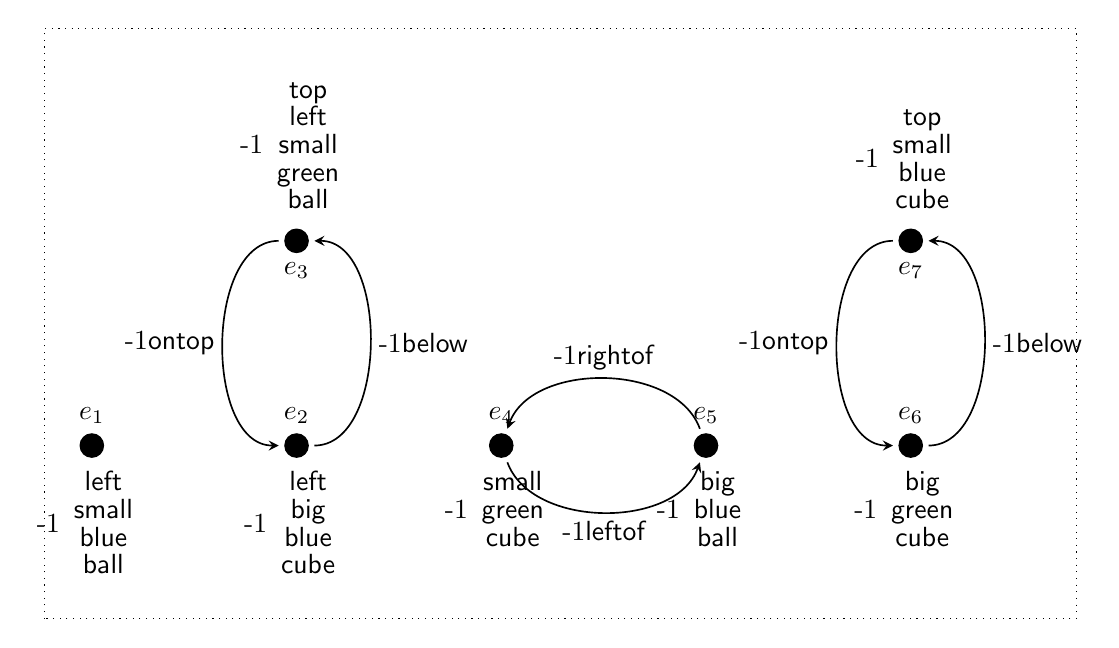
\begin{tikzpicture}
  [
    n/.style={circle,fill,draw,inner sep=3pt,node distance=2.6cm},
    aArrow/.style={->, >=stealth, semithick, shorten <= 2pt, shorten >= 2pt},
  ]
 \node[n,label=above:$e_1$,label=below:{
    \relsize{-1}$\begin{array}{c}
      \nLeft\\[-2pt]
      \nSmall\\[-2pt] 
      \nBlue \\[-2pt] 
      \nBall\end{array}$}] (a) {};

 \node[n,label=above:$e_2$,label=below:{
    \relsize{-1}$\begin{array}{c}
      \nLeft\\[-2pt]
      \nBig\\[-2pt] 
      \nBlue\\[-2pt] 
      \nCube\end{array}$}, right of=a] (b) {};

 \node[n,label=below:$e_3$,label=above:{
    \relsize{-1}$\begin{array}{c}
      \nTop\\[-2pt]
      \nLeft\\[-2pt]
      \nSmall\\[-2pt] 
      \nGreen\\[-2pt] 
      \nBall\end{array}$}, above of=b] (c) {};

 \node[n,label=above:$e_4$,label=below:{
    \relsize{-1}$\begin{array}{c}
      \nSmall\\[-2pt] 
      \nGreen\\[-2pt] 
      \nCube\end{array}$}, right of=b] (d) {};

 \node[n,label=above:$e_5$,label=below:{
    \relsize{-1}$\begin{array}{c}
      \nBig\\[-2pt] 
      \nBlue\\[-2pt] 
      \nBall\end{array}$}, right of=d] (e) {};

 \node[n,label=above:$e_6$,label=below:{
    \relsize{-1}$\begin{array}{c}
      \nBig\\[-2pt] 
      \nGreen\\[-2pt] 
      \nCube\end{array}$}, right of=e] (f) {};

 \node[n,label=below:$e_7$,label=above:{
    \relsize{-1}$\begin{array}{c}
      \nTop\\[-2pt]
      \nSmall\\[-2pt] 
      \nBlue\\[-2pt] 
      \nCube\end{array}$}, above of=f] (g) {};

 \draw [aArrow,bend right=90] (b) to node[auto,swap]{\relsize{-1}$\nBelow$} (c);
 \draw [aArrow,bend right=90] (c) to node[auto,swap]{\relsize{-1}$\nOntop$} (b);

 \draw [aArrow,bend right=70] (d) to node[auto,swap]{\relsize{-1}$\nLeftof$} (e);
 \draw [aArrow,bend right=70] (e) to node[auto,swap]{\relsize{-1}$\nRightof$} (d);

 \draw [aArrow,bend right=90] (f) to node[auto,swap]{\relsize{-1}$\nBelow$} (g);
 \draw [aArrow,bend right=90] (g) to node[auto,swap]{\relsize{-1}$\nOntop$} (f);

 \draw[dotted] (-.6,-2.2) rectangle (12.5,5.3);

 \end{tikzpicture}
\caption{Modelo relacional del Contexto \ref{GRE3D7-stimulus-cap2}}
\label{GRE3D7-stimulus-graph}
%\end{minipage}
\end{center}
\end{figure}

Algoritmos de refinamiento para GER se basan en la siguiente idea b\'asica:
dada una escena $S$, los objetos que aparecen en $S$ son sucesivamente
clasificados de acuerdo con sus propiedades en clases m\'as y m\'as finas. 
Una descripci\'on (en alg\'un lenguaje formal de $\mathcal{L}$) de cada
clase se calcula cada vez que una clase es refinada. El procedimiento siempre
se detiene cuando el conjunto de clases se estabiliza, es decir, no se puede hacer m\'as refinamiento
con la informaci\'on disponible en la escena \footnote{Por supuesto, si s\'olo estamos interesados en una expresi\'on referencial de un objeto dado, se puede detener el procedimiento en cuanto el objetivo es el
   \'unico elemento de alguna de las clases.}

Si el elemento target est\'a en
una clase singleton, entonces la descripci\'on formal de esa clase es un
expresi\'on referencial; de lo contrario el target no puede ser un\'{i}vocamente
descripto (en $\mathcal{L}$).

Est\'a claro que una escena puede ser codificada en diferentes formas como un
modelo relacional (por ejemplo, en \ref{GRE3D7-stimulus-cap2}, podr\'{i}amos argumentar que
$e_1$ es tambi\'en \emph{leftof} $e_2$, pero no lo consideramos porque no se estan 
tocando en la imagen). El algoritmo asume que estas cuestiones se han resuelto y que el modelo codifica una representaci\'on adecuada de la escena que
queremos describir. Por otra parte, vamos a suponer que todas las relaciones son
\emph{binarias}. No vamos a considerar las relaciones de aridad mayor que
dos (relaciones de mayor aridad pueden codificarse como relaciones binarias v\'{i}a
reificaci\'on, si es necesario).

%On termination, the algorithm computes what are called the
%$\mathcal{L}$-similarity classes of the input model $\gM$.
%Intuitively, the referring expression ``\textsf{ball}'' and ``\textsf{cube}''  are more specific and then contain more information than $\top$.


Tras la resoluci\'on, el algoritmo calcula lo que se llama la
$\mathcal{L}$ - clases de semejanza del modelo de entrada de $\gM$.\\

%There is many $\mathcal{L}$, we will name $\alc$ and $\el$

%ACA VOY A PONER gramatica para generar... ALC y EL no quedaria bien aca, hay que ver lo agregamos antes o no hace falta
%In what follows, we use formulas of the $\el$ description logic
%language
En lo que sigue, se utilizan f\'ormulas de la descripci\'on de la l\'ogica $\el$
~\cite{baad:desc03} para describir las clases de refinamiendo
\footnote{N\'otese, sin embargo, que el lenguaje formal particular usado es
   independiente del algoritmo principal, y diferentes funciones
  add$_{\mathcal{L}}$($\varphi$,\RE) se pueden utilizar dependiendo
   de la l\'ogica en cuesti\'on.}. como se discuti\'o 
en~\cite{arec2:2008:Areces}, 
este lenguaje es adecuado para describir
RE conjuntivas y relacionales, que son lo que encontramos en los corpus.

  La entrada al algoritmo ser\'a un modelo $\mathcal{M} =
 \tup{\Delta, \interp{\cdot}}$, donde $\Delta$ es el dominio no vac\'io de objetos de la imagen,
 $\interp{\cdot}$ es una funci\'on de interpretaci\'on que asigna a todas las propiedades de la escena su extensi\'on.
 Por ejemplo, la escena mostrada en la Figura~\ref{GRE3D7-stimulus-cap2} podr\'ia ser representada por el modelo
 $\gM=\tup{\Delta,\interp{\cdot}}$ mostrado en la 
 Figura~\ref{GRE3D7-stimulus-graph}; donde+- $\Delta =
 \{e_1,\ldots,e_7\}$, e $\interp{\textsf{red}}$ is $\{e_2, e_4, e_5,
 e_7\}$.

Se llama extensi\'on de una f\'ormula al conjunto de objetos que la hacen v\'alida.

$\top$ es una f\'ormula que representa la descripci\'on m\'as general, cuya
interpretaci\'on incluye todos los elementos del modelo. Se podr\'ia realizar
como la ER con el sustantivo
``\textsf{cosa}''. Decimos que una f\'ormula es
\emph{subsumida} por otras f\'ormulas, cuando su extensi\'on puede ser cubierta por la
union de las extensiones de las otras f\'ormulas. Por ejemplo, en la
Figura~\ref{GRE3D7-stimulus-cap2}, $\top$ es subsumida por ``\textsf{esfera}'' y
``\textsf{cubo}'', porque $\interp{\top}$ = $\interp{\textsf{esfera}}
\cup \interp{\textsf{cube}}$.
%= $\{e_2, e_4, e_6, e_7\}$, it is $\{e_1, e_2, e_3, e_4, e_5, e_6, e_7\}$ = $\{e_1, e_3, e_5\} \cup \{e_2, e_4, e_6, e_7\}$. 
Intuitivamente la f\'ormula ``\textsf{cubo}'' o ``\textsf{esfera}'' tienen m\'as informaci\'on que $\top$, para cada elemento de $\top$, hay una f\'ormula que d\'a m\'as informaci\'on, digamos ``\textsf{cubo}'' es m\'as informativa que ``\textsf{cosa}''.\\

%In the following we will explain an example of execusion of the
%algorithm shown in Figure
%A continuaci\'on vamos a explicar un ejemplo de ejecusi\'on del
%algoritmo mostrado en la Figura~\ref{algoritmoOriginal} considerando la l\'ogica 
%$\el$ como language. Este algoritmo fue presentado en
%~\cite{arec2:2008:Areces}.
%
%\begin{figure}[h!]
%\begin{center}
%\includegraphics[width=\textwidth]{images/algoritmoOriginal.png}
%\end{center}
%\vspace*{-2em}
%\caption{Algoritmo para GER con l\'ogicas de descripci\'on}
%\label{algoritmoOriginal}
%\end{figure}

%\subsection{Ejemplo de ejecuci\'on}
%
%
%
%\textcolor{blue}{no se si poner aca un ejemplo, si poner el texto y las im\'agenes en otro apendice... o ponerlas mas chiquitas en varias columnas, asi queda feo}\\
%Vamos a ejecutar el algoritmo para la Figura~\ref{GRE3D7-stimulus-cap2},
%el algoritmo comienza con una lista fija de propiedades y relaciones, supongamos que
%esas listas son las siguientes:
%
%propiedades ordenadas (prop): \textsf{ball}, \textsf{cube}, \textsf{red}, \textsf{yellow}, \textsf{small}, \textsf{large}.\\
%relaciones ordenadas (rel): \textsf{leftof}, \textsf{rightof}, \textsf{ontopof}, \textsf{bellowof}.
%
%%\begin{figure}
%%\begin{center}	
%%\includegraphics[width=.5\textwidth]{images/22.jpg}
%%\end{center}
%%\vspace*{-1.5em}
%%\caption{Escena 3D de figuras geom\'etricas}\label{figure22}
%%\end{figure}
%
%%\begin{figure}
%%\begin{minipage}[b]{0.6\linewidth}
%%\centering
%%\begin{tikzpicture}
%%  [
%%    n/.style={circle,fill,draw,inner sep=3pt,node distance=1.4cm},
%%    aArrow/.style={->, >=stealth, semithick, shorten <= 2pt, shorten >= 2pt},
%%  ]
%% \node[n,label=above:$e_1$,label=below:{
%%    \relsize{-1}$\begin{array}{c}
%%      \nLeft\\[-2pt]
%%      \nSmall\\[-2pt] 
%%      \nYellow \\[-2pt] 
%%      \nBall\end{array}$}] (a) {};
%
%% \node[n,label=above:$e_2$,label=below:{
%%    \relsize{-1}$\begin{array}{c}
%%      \nLeft\\[-2pt]
%%      \nSmall\\[-2pt] 
%%      \nRed\\[-2pt] 
%%      \nCube\end{array}$}, right of=a] (b) {};
%
%% \node[n,label=below:$e_3$,label=above:{
%%    \relsize{-1}$\begin{array}{c}
%%      \nTop\\[-2pt]
%%      \nLeft\\[-2pt]
%%      \nSmall\\[-2pt] 
%%      \nYellow\\[-2pt] 
%%      \nBall\end{array}$}, above of=b] (c) {};
%
%% \node[n,label=above:$e_4$,label=below:{
%%    \relsize{-1}$\begin{array}{c}
%%      \nBig\\[-2pt] 
%%      \nRed\\[-2pt] 
%%      \nCube\end{array}$}, right of=b] (d) {};
%
%% \node[n,label=above:$e_5$,label=below:{
%%    \relsize{-1}$\begin{array}{c}
%%      \nBig\\[-2pt] 
%%      \nRed\\[-2pt] 
%%      \nBall\end{array}$}, right of=d] (e) {};
%
%% \node[n,label=above:$e_6$,label=below:{
%%    \relsize{-1}$\begin{array}{c}
%%      \nSmall\\[-2pt] 
%%      \nYellow\\[-2pt] 
%%      \nCube\end{array}$}, right of=e] (f) {};
%
%% \node[n,label=above:$e_7$,label=below:{
%%    \relsize{-1}$\begin{array}{c}
%%      \nSmall\\[-2pt] 
%%      \nRed\\[-2pt] 
%%      \nCube\end{array}$}, right of=f] (g) {};
%
%% \draw [aArrow,bend right=90] (b) to node[auto,swap]{\relsize{-1}$\nBelow$} (c);
%% \draw [aArrow,bend right=90] (c) to node[auto,swap]{\relsize{-1}$\nOntop$} (b);
%
%% \draw [aArrow,bend right=30] (d) to node[auto,swap]{\relsize{-1}$\nLeftof$} (e);
%% \draw [aArrow,bend right=30] (e) to node[auto,swap]{\relsize{-1}$\nRightof$} (d);
%
%% \draw [aArrow,bend right=30] (f) to node[auto,swap]{\relsize{-1}$\nLeftof$} (g);
%% \draw [aArrow,bend right=30] (g) to node[auto,swap]{\relsize{-1}$\nRightof$} (f);
%
%% \draw[dotted] (-.4,-1.7) rectangle (7.5,3.3);
%
%% \end{tikzpicture}
%%\caption{La escena como modelo relacional}\label{GRE3D7-stimulus-graph}
%%\end{minipage}
%%\end{figure}
%
%
%El algoritmo siempre termina, y devuelve ER un conjunto de f\'ormulas que describe cada elemento en el dominio (si existe esa f\'ormula). \\
%
%En el comienzo ER=$\{\top\}$ y $\interp{\top}$ = $\{e_1, e_2, e_3, e_4, e_5, e_6, e_7\}$ como se puede ver en la Figura~\ref{fig-modelo}.\\
%
%ACA
%\begin{figure}[ht]
%\begin{minipage}[b]{0.45\linewidth}
%\centering
%\includegraphics[width=\textwidth]{images/22.jpg}
%\vspace*{1cm}
%%\caption{Input scene}
%\label{GRE3D7-stimulus-22}
%\end{minipage}
%%\hspace*{-0.35cm}
%\begin{minipage}[b]{0.6\linewidth}
%\centering
%%\begin{figure}[ht]
%%\begin{center}
%\frame{\includegraphics[width=8cm]{images/modelo.png}}\\[0pt]
%\caption{Modelo de la Figura \ref{GRE3D7-stimulus-22}}
%\label{fig-modelo}
%\end{minipage}
%\end{figure}
%El primer bucle del algoritmo es en las propiedades. Para cada propiedad hace add$_\el$ ($\varphi$, RE), las propiedades at\'omicas se muestran en la Figura~\ref{fig-modelo2}.
%
%\begin{figure}[ht]
%\begin{center}
%\frame{\includegraphics[width=8cm]{images/modelo2.png}}\\[0pt]
%\caption{Propiedades proposicionales en cuadro rojo, las del primer ciclo del algoritmo}
%\label{fig-modelo2}
%\end{center}
%\end{figure}
%
%La f\'ormula $\varphi$ se a\~nadir\'a a ER si su interpretaci\'on tiene al menos un elemento, a continuaci\'on, para cada f\'ormula
 %$\psi$ en ER la conjunci\'on
%$\varphi  \wedge \psi$ no necesita estar subsumida in ER, la $\interp{\varphi \cup \psi}$ no tiene que ser vac\'io, y su interpretaci\'on tiene que ser distinta de $\interp{\psi}$. Luego las f\'ormulas subsumidas se borran.
%
%La primer propiedad es \textsf{ball}, ER = \{$\top$, \textsf{ball}\}, se ven los elementos de ``ball'' en un recuadro en la Figura~\ref{fig-modelo3}.
%
%\begin{figure}[ht]
%\begin{center}
%\frame{\includegraphics[width=8cm]{images/modelo3.png}}\\[0pt]
%\caption{El cuadro indica cuales son ``ball''}
%\label{fig-modelo3}
%\end{center}
%\end{figure}
%
%La siguiente propiedad es \textsf{cube}, ER = \{$\top$, \textsf{ball}, \textsf{cube}\}, pero ahora la $\interp{\textsf{ball}}$ = $\{e_1, e_3, e_5\}$, $\interp{\textsf{cube}}$ = $\{e_2, e_4, e_6, e_7\}$, quedando las particiones como se muestra en la Figura~\ref{fig-modelo4}
%\begin{figure}[ht]
%\begin{center}
%\frame{\includegraphics[width=8cm]{images/modelo4.png}}\\[0pt]
%\caption{Cuadros indicando ``ball'' y ``cube''}
%\label{fig-modelo4}
%\end{center}
%\end{figure}
%Ahora podemos borrar $\top$, porque es subsumida (esta cubierta por) las otras dos f\'ormulas. La siguiente propiedad es  \textsf{red}, $\interp{\textsf{red}}$ es: $\{e_2, e_4, e_5, e_7\}$, haciendo la intersecci\'on con la $\interp{.}$ de cada f\'ormula en ER obtenemos, $\{e_5\}$ y $\{e_2, e_4, e_7\}$, ER = $\{\textsf{ball}, \textsf{cube}, \textsf{ball} \wedge \textsf{red}, \textsf{cube} \wedge \textsf{red}\}$, las particiones actuales se pueden ver en la Figura~\ref{fig-modelo9}.
%\begin{figure}[ht]
%\begin{center}
%\frame{\includegraphics[width=8cm]{images/modelo9.png}}\\[0pt]
%\caption{Cuadros indicando ``ball'', ``cube'' y ``red''}
%\label{fig-modelo9}
%\end{center}
%\end{figure}
%
%Siguiendo con \textsf{yellow}, tenemos, $\interp{\textsf{yellow}}$ = $\{e_1, e_3, e_6\}$ y obtenemos ER = $\{\textsf{ball} \wedge \textsf{yellow}, \textsf{cube} \wedge \textsf{yellow}, \textsf{ball} \wedge \textsf{red}, \textsf{cube} \wedge \textsf{red}\}$. 
%Note que aqu\'i ya borramos la f\'ormula \textsf{ball} porque estaba subsumida, y la f\'ormula \textsf{cube} tambi\'en. Se muestran particiones en Figura~\ref{fig-modelo10}.
%
%\begin{figure}[ht]
%\begin{center}
%\frame{\includegraphics[width=8cm]{images/modelo10.png}}\\[0pt]
%\caption{Cuadros indicando ``ball'', ``cube'', ``red'' y ``yellow''}
%\label{fig-modelo10}
%\end{center}
%\end{figure}
%
%Haciendo lo mismo con \textsf{small} tenemos ER = $\{\textsf{ball} \wedge \textsf{yellow} \wedge \textsf{small}, \textsf{cube} \wedge \textsf{yellow} \wedge \textsf{small}, \textsf{ball} \wedge \textsf{red}, \textsf{cube} \wedge \textsf{red}, \textsf{cube} \wedge \textsf{red} \wedge \textsf{small}\}$, como se puede ver en Figura~\ref{fig-modelo11}.
%\begin{figure}[ht]
%\begin{center}
%\frame{\includegraphics[width=8cm]{images/modelo11.png}}\\[0pt]
%\caption{Cuadros indicando ``ball'', ``cube'', ``red'', ``yellow'', ``small'' y ``large''}
%\label{fig-modelo11}
%\end{center}
%\end{figure}
%
%La siguiente propiedad es \textsf{large} as\'i, tenemos ER = $\{\textsf{ball} \wedge \textsf{yellow} \wedge \textsf{small}, \textsf{cube} \wedge \textsf{yellow} \wedge \textsf{small}, \textsf{ball} \wedge \textsf{red}, \textsf{cube} \wedge \textsf{red} \wedge \textsf{large}, \textsf{cube} \wedge \textsf{red} \wedge \textsf{small}\}$. Aqu\'i no podemos agregar \textsf{large} a la f\'ormula $\textsf{red} \wedge \textsf{cube}$ porque su interpretaci\'on tiene un solo elemento, y la condici\'on dice que es necesario tener m\'as de uno.
%
%Hasta ahora ER = $\{\textsf{ball} \wedge \textsf{yellow} \wedge \textsf{small}, \textsf{cube} \wedge \textsf{yellow} \wedge \textsf{small}, \textsf{ball} \wedge \textsf{red}, \textsf{cube} \wedge \textsf{red} \wedge \textsf{large}, \textsf{cube} \wedge \textsf{red} \wedge \textsf{small}\}$ 
%y tenemos las siguientes extensiones: $\{e_1, e_3\}, \{e_6\}, \{e_5\}, \{e_4\}, \{e_2, e_7\}$ respectivamente. 
%Hay dos f\'ormulas que a\'un pueden ser refinadas, $\textsf{ball} \wedge \textsf{yellow} \wedge \textsf{small}$ y $\textsf{cube} \wedge \textsf{red} \wedge \textsf{small}$ 
%debido a que tienen m\'as de un elemento cada una, por lo que entran en el ciclo, while del algoritmo 1, en la l\'inea 4. Ahora es el turno de las relaciones, la primera de ellas es \textsf{leftof}, para cada f\'ormula $\varphi$ en ER trataremos de hacer add$_\el$ ($\exists \textsf{leftof}.\varphi$, RE). Notar que $\psi$ solo puede ser $\textsf{ball} \wedge \textsf{yellow} \wedge \textsf{small}$ o $\textsf{cube} \wedge \textsf{red} \wedge \textsf{small}$ porque esos son los que su interpretaci\'on tiene m\'as de un elemento. 
%\begin{figure}[ht]
%\begin{center}
%\frame{\includegraphics[width=8cm]{images/modelo15.png}}\\[0pt]
%\caption{Cuadros indicando ``ball'', ``cube'', ``red'', ``yellow''...}
%\label{fig-modelo15}
%\end{center}
%\end{figure}
%
%
%No hay
%%because those are the ones that its interpretation have more than one element. There is not 
%$\varphi$ y $\psi$ que puedan ser aplicadas. Continuando con \textsf{rightof} agregamos $\textsf{cube} \wedge \textsf{yellow} \wedge \textsf{small} \wedge \exists \textsf{rightof}. \textsf{cube} \wedge \textsf{red} \wedge \textsf{small}$, y asi con \textsf{topof} agregamos $\textsf{small} \wedge \textsf{red} \wedge \textsf{cube} \wedge \exists \textsf{ontop}. \textsf{small} \wedge \textsf{yellow} \wedge \textsf{ball}$ y el algoritmo termina con ER = $\{\textsf{ball} \wedge \textsf{yellow} \wedge \textsf{small}, \textsf{cube} \wedge \textsf{yellow} \wedge \textsf{small}, \textsf{ball} \wedge \textsf{red}, \textsf{cube} \wedge \textsf{red} \wedge \textsf{large}, \textsf{cube} \wedge \textsf{red} \wedge \textsf{small}, \textsf{cube} \wedge \textsf{yellow} \wedge \textsf{small} \wedge \exists \textsf{rightof}. \textsf{cube} \wedge \textsf{red} \wedge \textsf{small}, \textsf{small} \wedge \textsf{red} \wedge \textsf{cube} \wedge \exists \textsf{ontop}. \textsf{small} \wedge \textsf{yellow} \wedge \textsf{ball}\}$, 
%aqu\'i todos los elementos est\'an en una clase singleton y no se puede hacer ning\'un refinamiento m\'as. 
%%can be applied to $cube \wedge red \wedge small$ but there is no formula which interpretation has more than one element to be apply with this one. The same happen for the other relations, so the algorithm ends.
%%its interpretation is $\{e_7\}$ with $\psi$ is $cube \wedge yellow \wedge small$, the others combinations can't be apply because they don't do true the preconditions. The following relation is rightof, 
%
%%leftof, rightof, ontopof, bellowof
%
%%At this point we already have the target in a singleton set. So the formula for it is ``red and ball'', and also for s6 which formula is ``yellow cube''.\\
%%As we show this algorithm depends of the order of properties and relations.\\
%\begin{figure}[ht]
%\begin{center}
%\frame{\includegraphics[width=8cm]{images/modelo16.png}}\\[0pt]
%\caption{Cuadros indicando ``ball'', ``cube'', ``red'', ``yellow''...}
%\label{fig-modelo16}
%\end{center}
%\end{figure}
%
%\begin{figure}[ht]
%\begin{center}
%\frame{\includegraphics[width=8cm]{images/modelo17.png}}\\[0pt]
%\caption{Cuadros indicando ``ball'', ``cube'', ``red'', ``yellow''...}
%\label{fig-modelo17}
%\end{center}
%\end{figure}
%
%Las expresiones referenciales encontradas son:\\
%
%$\textsf{ball} \wedge \textsf{yellow} \wedge \textsf{small}$ representa $e_1$ \\
%$\textsf{cube} \wedge \textsf{yellow} \wedge \textsf{small}$ representa $e_6$ \\
%$\textsf{ball} \wedge \textsf{red}$ representa $e_5$ \\
%$\textsf{cube} \wedge \textsf{red} \wedge \textsf{large}$ representa $e_4$ \\
%$\textsf{cube} \wedge \textsf{red} \wedge \textsf{small}$ representa $\{e_2,e_7\}$  \\
%$\textsf{cube} \wedge \textsf{yellow} \wedge \textsf{small} \wedge \exists \textsf{rightof}. \textsf{cube} \wedge \textsf{red} \wedge \textsf{small}$ representa $e_6$ \\
%$\textsf{small} \wedge \textsf{red} \wedge \textsf{cube} \wedge \exists \textsf{ontop}. \textsf{small} \wedge \textsf{yellow} \wedge \textsf{ball}$ representa $e_2$ \\
%



\section{Aproximaciones emp\'iricas a la soluci\'on de GER}
\label{sec:trabajos_empiricos}
\subsection{Corpus existente}
\label{sec:corpus2}
\label{sec:corpusTUNA}

%was the first prominent REG corpus to be made publicly available for research purposes. The corpus was developed in a series of general-purpose controlled experiments, containing 2280 descriptions produced by 60 speakers in two domains (1200 descriptions of furniture items and 1080 descriptions of people's photographs). TUNA does not contain relational descriptions, and it is possibly the only resource of this kind to include situations of reference to sets. The TUNA corpus has been extensively used in a series of shared tasks

TUNA \cite{tuna-corpus} fue el primer corpus prominente para GER disponible p\'ublicamente con fines de investigaci\'on. El corpus fue desarrollado en una serie de experimentos controlados de prop\'osito general, contiene 2.280 descripciones producidas por 60 personas en dos dominios (1.200 expresiones referenciales de im\'agenes de muebles y 1080 expresiones referenciales de fotograf\'ias de personas situadas en una grilla). Se muestran ejemplos de im\'agenes en Figuras \ref{fig-TUNA-furniture} y \ref{fig-TUNA-people}. El corpus TUNA no contiene descripciones relacionales, y es posiblemente el \'unico recurso de este tipo que incluye situaciones de referencia a conjuntos. Este corpus se ha utilizado ampliamente en una serie de desaf\'ios \cite{reg2009}. 

\begin{figure}
\begin{minipage}[t]{0.5\linewidth}
\centering
\includegraphics[width=\textwidth]{images/largeGreyChair.jpg}\\[0pt]
\caption{Imagen del TUNA corpus (muebles)}
\label{fig-TUNA-furniture}
\vspace*{.1cm}
\end{minipage}
\hspace*{0cm}
\begin{minipage}[t]{0.5\linewidth}
\centering
\includegraphics[width=\textwidth]{images/tuna-people.jpg}\\[0pt]
\caption{Imagen del TUNA corpus (personas)}
\label{fig-TUNA-people}
\end{minipage}
\end{figure}


\label{sec:corpusGRE}
%were developed in a series of web-based experiments primarily focussed on the study of relational descriptions. GRE3D3 contains 630 descriptions produced by 63 speakers, and GRE3D7 contains 4480 descriptions produced by 287 speakers, making it the largest of its kind to date. The GRE3D domain consists of simple visual scenes containing only two kinds of objects (boxes and spheres) with limited variation in colour and size. In each scene, there is only one possible spatial relation between target and the nearest landmark. Both corpora contain atomic and relational descriptions.
GRE3D3 y su extensi\'on GRE3D7 \cite{gre3d3,gre3d7} se desarrollaron en una serie de experimentos basados en la web, se centraron principalmente en el estudio de las descripciones relacionales. GRE3D3 contiene 630 descripciones producidas por 63 personas y GRE3D7 contiene 4.480 descripciones producidas por 287 personas, y es el corpus m\'as grande de este tipo hasta la fecha. El dominio del GRE3D3 consta de escenas visuales simples que contienen s\'olo dos tipos de objetos (cubos y esferas) con variaci\'on limitada en color y tama\~no. En cada escena, s\'olo hay una posible relaci\'on espacial entre el target y el landmark m\'as cercano. Ambos corpus contienen descripciones at\'omicas y relacionales. Ejemplo de im\'agenes del GRE3D3 y GRE3D7 se muestran en las Figuras \ref{fig-GRE3D3} y \ref{fig-GRE3D7}.
%\begin{minipage}[b]{0.45\linewidth}

\begin{figure}
\begin{minipage}[b]{0.5\linewidth}
\centering
\includegraphics[width=\textwidth]{images/GRE3D3.png}\\[0pt]
\caption{Imagen del GRE3D3}
\label{fig-GRE3D3}
\vspace*{-0.7cm}
\end{minipage}
\hspace*{0cm}
\begin{minipage}[b]{0.5\linewidth}
\centering
\includegraphics[width=\textwidth]{images/3.jpg}\\[0pt]
\caption{Imagen del GRE3D7}
\label{fig-GRE3D7}
\end{minipage}
\end{figure}

%\vspace*{3cm}

\label{sec:corpusSTARS}
%and its extension Stars2 were collected for the study of referential overspecification (particularly in the case of relational descriptions). Stars was developed in a pilot web-based experiment, containing 704 descriptions produced by 64 speakers.  The more comprehensive Stars2 data set was produced in dialogue situations involving subject pairs, and it contains 884 descriptions produced by 56 speakers. Both domains make use of simple visual scenes containing up to four object types (e.g., stars, boxes, cones and spheres) with limited variation in colour and size. Differently from other REG corpora, however, Stars/2 includes a considerable number of complex situations of reference involving up to three objects, as in `the box near the sphere, next to the cone'.http://ppgsi.each.usp.br/arquivos/RelTec/PPgSI-002_2014.pdf y http://ppgsi.each.usp.br/arquivos/RelTec/PPgSI-001_2015.pdf
Stars \cite{stars-mutual-disamb} y su extensi\'on Stars2 se recolectaron para el estudio de la sobre-especificaci\'on (particularmente en el caso de las descripciones relacionales). Stars se desarroll\'o en un experimento piloto basado en la web, contiene 704 descripciones producidas por 64 personas. El conjunto de datos Stars2 es m\'as completo y se obtuvo de situaciones de di\'alogo que implicaban a dos personas, contiene 884 descripciones producidas por 56 participantes. Ambos dominios hacen uso de escenas visuales simples que contienen tres tipos de objetos (por ejemplo para Stars, estrellas, cuadrados y c\'irculos y para Stars2 cubos, conos y esferas) con variaci\'on limitada en color y tama\~no. A diferencia de otros corpus para GER, Stars/2 incluyen un n\'umero considerable de situaciones complejas de referencia en que participan hasta tres objetos, como en ``el cubo cerca de la esfera, al lado del cono''. Ejemplos de imagenes se muestran en las Figuras \ref{fig-STARS} y \ref{fig-STARS2}.

\begin{figure}
\begin{minipage}[b]{0.5\linewidth}
\centering
\includegraphics[width=\textwidth]{images/STARS.png}\\[0pt]
\caption{Imagen de Stars corpus}
\label{fig-STARS}
%\vspace*{1cm}
\end{minipage}
\hspace*{0cm}
\begin{minipage}[b]{0.5\linewidth}
\centering
\includegraphics[width=\textwidth]{images/STARS2.png}\\[0pt]
\caption{Imagen de Stars2 corpus}
\label{fig-STARS2}
\end{minipage}
\end{figure}


\label{sec:corpusZOOM}
%were developed in a series of web-based experiments primarily focussed on the study of relational descriptions. GRE3D3 contains 630 descriptions produced by 63 speakers, and GRE3D7 contains 4480 descriptions produced by 287 speakers, making it the largest of its kind to date. The GRE3D domain consists of simple visual scenes containing only two kinds of objects (boxes and spheres) with limited variation in colour and size. In each scene, there is only one possible spatial relation between target and the nearest landmark. Both corpora contain atomic and relational descriptions.
El ZOOM corpus se desarrollar\'o en un trabajo conjunto con la Universidad de Sao Paulo, contiene ER para 20 mapas de las ciudades de Lisboa y Madrid, fue realizado en la web, y contiene ER de targets singulares y plurales, con y sin zoom, en 2 idiomas: espa\~nol y portugu\'es. El corpus portugues contiene 100 ER por mapa, y el espa\~nol 80. Ejemplos de esos mapas se muestran en las Figuras{rest-singular2x} y \ref{rest-plural2x}.


\begin{figure}
\begin{minipage}[b]{0.5\linewidth}
\centering
\includegraphics[width=\textwidth]{figures/rest-singular2x.png}\\[0pt]
\caption{Target singular con zoom 2X}
\label{rest-singular2x}
\end{minipage}
\vspace*{.1cm}
\begin{minipage}[b]{0.5\linewidth}
\centering
\includegraphics[width=\textwidth]{figures/rest-plural2x.png}\\[0pt]
\caption{Target plural con zoom 2X}
\label{rest-plural2x}
\end{minipage}
\end{figure}





\subsection{Trabajos emp\'iricos en el \'area}
\label{sec:trab_emp}

%http://link.springer.com/chapter/10.1007/978-3-642-15573-4_9
%http://www.jetteviethen.net/papers/DaleViethen2010chapter.pdf

La investigaci\'on presentada en \cite{viethen-phd} se basa en dos premisas fundamentales: que la investigaci\'on
en la generaci\'on autom\'atica de expresiones referenciales debe esforzarse por lograr
sistemas que den salidas tan similar a la humana como sea posible; y que, para ello, debemos
esforzarnos para modelar el comportamiento humano como se puede observar en corpora.

La adopci\'on de estas premisas sirve para dos fines: en primer lugar, mejora la adecuaci\'on
de la salida de algoritmos de GER para el objeto target imitando la capacidad humana
de producir referencias adecuadas; y en segundo lugar, el estudio de corpus de datos producidos por humanos
 y algoritmos en desarrollo que pueden replicar estos datos podr\'ian
acercarnos a la comprensi\'on de que es lo que hacen los humanos cuando dan una ER.

Se\~nala que el cl\'asico algoritmo de GER y la mayor parte de sus descendientes no se basaron ni evaluaron contra datos producidos por humanos. Ellos se basaron en una visi\'on bastante minimalista de lo que se necesita
para que una expresi\'on referencial sea \'optima, concentr\'andose en la eficiencia computacional 
 y descripciones breves como sus principales preocupaciones.

 Existe un peque\~no n\'umero de enfoques que 
 se basaron en observaciones del comportamiento de referencia general humana
que obtuvieron a partir de experimentos psicoling\"u\'isticos, pero de nuevo no fueron evaluados
contra datos humanos.

Los algoritmos que se presentaron a los desaf\'ios de evaluaci\'on \cite{gatt-balz-kow:2008:ENLG} y \cite{reg2009}
fueron probados en el TUNA-Corpus, y algunos de ellos
tambi\'en tuvieron en cuenta los patrones que se encontraban en el conjunto del desarrollo. Pero hay una serie de preocupaciones en torno a la pregunta de si el TUNA-Corpus, y la forma de salida de los sistemas que se compar\'o 
en los desaf\'ios eran ideales para una evaluaci\'on de la adecuaci\'on descriptiva de GER.
%saque esto porque no se entiende
%A partir de los desaf\'ios que se describen en m\'as detalle y para evaluarlos en una serie de datos m\'as grande
%que contiene m\'as de una expresi\'on referencial para cada elemento est\'imulo.
Aborda tres \'areas principales en las que los corpus se puede utilizar para
promover el objetivo de la semejanza humana en la investigaci\'on sobre generaci\'on de expresiones referenciales:
evaluaci\'on, la recolecci\'on de corpus y an\'alisis y modelizaci\'on estad\'istica de
datos de corpus.
Comenz\'o con el an\'alisis del estado del arte de la investigaci\'on en
la generaci\'on de descripciones distintivas, trabaj\'o con relaciones espaciales y en el trabajo us\'o datos de corpus. Examin\'o una serie de opciones metodol\'ogicas que tienen que hacerse cuando se trabaja con los corpus de GER. Aqu\'i, explor\'o diferentes opciones para los desaf\'ios de recopilaci\'on de corpus, que se centran en torno al equilibrio que se necesita
entre el control de los par\'ametros experimentales tanto como sea necesario
y mantener la configuraci\'on de lo m\'as natural posible. Discuti\'o una serie de conceptos
que son de importancia para el an\'alisis de corpora de GER, tales como la naturalidad de diferentes
propiedades de los objetos, y las nociones de minimalidad y cuestiones de sobre-especificaci\'on de expresiones referenciales. Por \'ultimo, analiz\'o diferentes maneras en que la salida de un sistema se puede
comparar con los datos de corpora, bajo la premisa de que el objetivo de la comparaci\'on es
para evaluar si el sistema podr\'ia tener un modelo adecuado del comportamiento humano para la generaci\'on de expresiones referenciales.
Realiz\'o una investigaci\'on en las tres \'areas donde se puede emplear corpora en GER: Evaluaci\'on de semejanza humana, recopilaci\'on y an\'alisis de corpus, y modelado de datos de corpus. Realiz\'o un experimento de evaluaci\'on con tres de los algoritmos cl\'asicos, (1989) Algoritmo Greedy de Dale (Greedy), Dale y Haddock (1991b), Algoritmo Relacional (ra) Y Dale y Reiter (1995) Algoritmo Incremental (IA), Se pusieron a prueba en cuanto a su capacidad de
replicar las expresiones referenciales se encuentran en un grupo relativamente peque\~no de corpus de expresiones referenciales
en un dominio visual de im\'agenes puestas en una grilla.
%de rejilla de cajones de armarios ling. 
En el an\'alisis de este experimento tuvo dos resultados principales: (1) que identic\'o en particular tres 
fen\'omenos que todav\'ia plantean importantes retos para los algoritmos GER con el objetivo de replicar
el comportamiento humano, y (2) que proporciona una plataforma para la discusi\'on de una serie de
dificultades que se presentan para la evaluaci\'on basada en corpus de GER. Esto result\'o en una serie
de criterios para el dise\~no de los dos corpus que el trabajo en el resto de la tesis.
Los tres fen\'omenos en las expresiones referenciales producidas por humanos que los
algoritmos probados no fueron capaces de replicar satisfactoriamente sobre-especificaci\'on,
relaciones espaciales, y comportamiento de voluntarios espec\'ificos. Ambos
Greddy y la IA fueron capaces de generar algo de la redundancia que se encontr\'o en el corpus.
 Ni Greedy ni el IA estaban dise\~nados para ser capaz de generar expresiones referenciales que contengan relaciones entre entidades, pero el ra fue dise\~nado para incluirlas. Sorprendentemente, el
ra no s\'olo fallo en generar cualquiera de las descripciones contenidas en el corpus de evaluaci\'on; sino tambi\'en que las descripciones que se gener\'o parec\'ian m\'as como enigmas cuyo objetivo era confundir a un oyente, m\'as que ayudar en
los intentos de se\~nalar el objetivo referente. 

Una valoraci\'on te\'orica de otras aproximaciones dise\~nados para manejar las relaciones estableci\'o que ninguno de ellos incluir\'ia una relaci\'on, si no es absolutamente necesaria para distinguir el target.
La tercera observaci\'on que el experimento dejo a la vista fue que la gente no siempre hace lo mismo en la misma situaci\'on. De hecho, incluso la misma persona podr\'ia describir el mismo target de diferente manera en distintas
circunstancias. 

 None of the algorithms tested were intended to take such inter- and
intra-speaker variation into account, and only very recently have implementations
of the
ia
begun to model speaker-preferences to some degree.

No se pretend\'ia que ninguno de los algoritmos de la prueba tomara en cuenta las variaciones entre-hablantes, ni del mismo hablante. Hay implementaciones del IA que han comenzado a agregar modelo de preferencias de hablante en alg\'un grado.

Los temas generales con evaluaci\'on basada en corpus que esta experiencia de evaluaci\'on dej\'o
al descubierto fueron (1) la interdependencia estrecha entre algoritmos y la
representaci\'on subyacente de conocimiento que utilizan, (2) el no-determinismo de la generaci\'on del lenguaje natural, (3) la cuesti\'on de c\'omo comparar la salida algoritmos con gold-standar, y (4) el dominio espec\'ifico de los algoritmos de GER.\\
La discusi\'on de estos temas ha dado lugar a la siguiente lista de Evaluaci\'on en GER basado en corpus:

1. Si el corpora est\'a destinado para ser reutilizado para la evaluaci\'on comparativa de diferentes
algoritmos, una representaci\'on subyacente del dominio debe ser proporcionada para ser usada por todos los algoritmos.

2. Si queremos confiar en los resultados, el corpus debe contener tantos casos como sea posible de tantos direntes hablantes como sea posible para cada escenario referencial. 
Esto es cierto si un algoritmo es evaluado en t\'erminos de ser capaz de generar una expresi\'on referencial que suene natural, o si est\'a probado por su probabilidad de pertenecer a un modelo espec\'ifico de conducta humana de referencia, mediante la comprobaci\'on de si se puede generar todas las descripciones en un corpus.

3. Si la probabilidad de un algoritmo de ser un modelo de la conducta humana de referencia
se eval\'ua, deben utilizarse m\'etricas basadas en recuento (RECALL) y precisi\'on (PRESITION). En este
caso, el conjunto completo de las descripciones que el algoritmo proporciona para cada
escenario de referencia en virtud de cualquier ajuste de par\'ametro debe ser comparado con el
conjunto de las descripciones contenidas en el corpus para el mismo escenario referencial.
Si la capacidad m\'as orientada a la aplicaci\'on para generar una referencia es similar a la humana
se ha de evaluar, s\'olo una descripci\'on por escenario.
Esto debe hacerse utilizando m\'etricas basadas en la precisi\'on para probar c\'omo muchos de las
descripciones dadas por los algoritmos est\'an contenidas en el corpus.
4. Algoritmos que son juzgados en un dominio espec\'ifico c, no se debe asumir como
f\'acilmente adaptable a otros dominios. Idealmente, los corpus que abarcan muchos diferentes
deben estar disponibles para las pruebas de los algoritmos que generalizan en distintos tipos de dominios.
Realiz\'o 2 corpus el GRE3D3 y el GRE3D7 descriptos en \ref{sec:corpus2}

Trabaj\'o con \'arboles de decisi\'on ...
\textcolor{blue}{Aca agregar otras personas que usaron corpus para generacion de ER, Ivandre... }

%http://www.lrec-conf.org/proceedings/lrec2012/pdf/152_Paper.pdf
En el trabajo \ref{ivandre-work-corpus} presentan 2 alternativas para aprender la seleccio\'on de atributos de una expresi\'on referencial a partir de corpus. Toma los caracter\'isticas de aprendizaje como el conjunto de valores enteros que representan el poder discriminativo de cada atributo (es decir, el n\'umero de distractores que cada atributo elimina por cada atributo que tiene el target, ejemplos son color, tama\~no, etc.) 
 %For instance, in a context set as
%seen in previous Example 1, assuming that we would like to
%refer to E4, the corresponding discriminatory power values
%would be defined as d type =1, d size =1 and d colour =3.
%In the first learning method, we will attempt to learn possible
%Pj orderings (defined as nominal values) that, if applied
%to  the  Incremental  algorithm,  would  produce  the  desired
%output L for each given input C. In the second method, we
%will  use  the  input  C  to  (binary)  decide  whether  to  select
%each attribute individually.  We will call these our
%Global and Individual AS  classifiers,  which  are  discussed  sepa-
%rately below

\subsection{M\'etricas de evaluaci\'on/comparaci\'on con corpus}
\label{sec:metricas_evaluacion}
Jordan y Walker usaron 25 veces la validaci\'on cruzada en 393 expresiones referenciales
de 13 de la Coco di\'alogos para probar diferentes combinaciones de caracter\'isticas. Ellos
medido la precisi\'on absoluta, siendo \'esta la proporci\'on de expresiones referenciales
generadas que son id\'enticas a las descripciones de referencia humanos producidos a partir de
el corpus. En el aislamiento, la intencional uencias factores desempe\~naron mejor (42,4\%
exactitud) que los otros dos conjuntos de caracter\'isticas (conjuntos de contraste: 30,4\% y conceptual
pactos: 28,9\%) y la combinaci\'on de los tres tipos de caracter\'isticas hicieron signicativa no inexactitud aumento (43,2\%). Sin embargo, lo que tuvo el mayor impacto fue cuarto,
independiente de la teor\'ia, el tipo de caracter\'isticas que registran informaci\'on al juicio espec\'ifico c, tales
como el juicio
Identificaci\'on
, El participante-diada, el hablante actual y el atributo exacta
valores de la referente de destino. En el aislamiento, esta colecci\'on de caracter\'isticas logra el 54,5\%
exactitud, y combin\'andolos con todos los otros tres tipos de caracter\'isticas s\'olo aumentaron
esta actuaci\'on al 59,9\%. Estos resultados apoyan leve a Jordan intencional
en
influencias modelo sobre los otros dos modelos, pero m\'as fuertemente sugieren que ninguno
de los modelos de capturar la variaci\'on en los datos muy bien
incursi\'on en el uso de la m\'aquina de aprendizaje para
reg
fue hecha por Stoia et al.
(2006). Ellos apuntan a la construcci\'on de un sistema de di\'alogo para un agente situado dando
instrucciones en un mundo virtual en 3D. Sin embargo, este enfoque no se centr\'o por lo
tanto en la selecci\'on de contenidos como en determinar la mejor forma de referencia a utilizar.
Utilizaron un aprendiz m\'aquina para entrenar a los \'arboles de decisi\'on que decidieron que determinador
utilizar, qu\'e tipo de cabeza para incluir en el sintagma nominal (por ejemplo, un pronombre o una
nombre com\'un) y si desea o no utilizar una frase modi sustantivo. La sem\'antica
contenido del modificador no estaba en cuesti\'on. Las funciones disponibles para la decisi\'on
alumnos de los \'arboles eran una mezcla de la historia del di\'alogo, contexto visual y tipo sem\'antico
informaci\'on sobre el referente objetivo. Entrenaron \'arboles de decisi\'on separados para de-
terminer, sustantivo principal y la elecci\'on modificador y les aplicaron secuencialmente, con cada \'arbol que tenga acceso a la salida del \'arbol anterior. Para el entrenamiento y autom\'atico
%evaluaci\'on que utilizan un conjunto de 1242 expresiones referenciales de una colecci\'on de di\'alogo
%Logues entre dos compan\~eros de conversaci\'on que llevaban a cabo la instrucci\'on
%tarea en el mismo mundo virtual como el sistema se emplea en adelante. Esta
%evaluaci\'on autom\'atica encontr\'o que los \'arboles de decisi\'on fueron capaces de igualar la humana datos en el 31\% de todos los casos. Como no estaban interesados ​​tanto en la semejanza humana
%de su sistema, pero sobre todo en su cacia e, tambi\'en realizaron un intr\'inseca
%Evaluaci\'on humana en la que se pidi\'o a los participantes para comparar la salida del sistema
%a las expresiones que se refieren humanos producidos en una l\'inea de base y al azar. El humano
%evaluadores juzgados 62,6\% de las expresiones que se refieren generados por el sistema para


Un n\'umero de los sistemas presentados a los desaf\'ios GER de evaluaci\'on basados
en el TUNA Corpus se basaron en los an\'alisis emp\'iricos del conjunto de entrenamiento. La mayor\'ia
de estos sistemas se basaban en la
ia y se utiliza un simple recuento de frecuencia de la
propiedades en el conjunto de entrenamiento para informar el orden en que Propie- del referente de destino
propie- deben ser juzgados (Kelleher, 2007; Spanger et al, 2007;. Fabbrizio et al., 2008;
Kelleher y Namee, 2008; de Lucena y Paraboni, 2008; Gerv como et al, 2008?.;
de Lucena y Paraboni, 2009). Un equipo, que yo era parte de, que se utiliza en frecuencia
funciones basadas en costos en el algoritmo gr\'afico-Based (Theune et al, 2007; Krahmer.
et al., 2008; Brugman et al., 2009). Bohnet (2007, 2008, 2009) nearest- combinado
vecino de aprendizaje con un enfoque brevedad completa, con el fin de elegir el m\'as corto
refiri\'endose expresi\'on que mejor se ajuste a los datos de entrenamiento para un determinado objetivo; y
utiliza un \'arbol de decisi\'on aprendido de los datos de entrenamiento para determinar din\'amicamente el
orden de preferencia para la
ia
. En 2008 y 2009, Bohnet adapta su brevedad completo al-
goritmo para que coincida con los participantes individuales, pero encontr\'o que la informaci\'on del participante
no se proporcion\'o de forma fiable en los datos de prueba. Fabbrizio et al. (2008) present\'o la
\'unico otro enfoque que intent\'o capturar las preferencias de c-altavoz espec\'ifico en
la brevedad completo y el algoritmo incrementales. Su enfoque completo brevedad recogi\'o
las descripciones m\'as cortas que estaba bien con m\'as frecuencia o m\'as recientemente utilizado por el
mismo orador, y su versi\'on de la
ia
basada en frecuencia usada altavoz espec\'i c
\'ordenes de preferencias. King (2008) y Herv\'e? Como y Gerv? As (2009) utilizaron evolutiva
programaci\'on para la tarea de selecci\'on de contenido, pero ambos se encontraron con muy limitado
el \'exito.

Investigaci\'on REG Pre-2000 dio poca o ninguna atenci\'on a la evaluaci\'on emp\'irica de algoritmos. M\'as recientemente, sin embargo, los estudios de evaluaci\'on REG han comenzado a realizar
m\'as y m\'as a menudo. Al parecer, la mayor\'ia de ellos se basaban en el supuesto de
(debatidas en la Secci\'on 7) que los algoritmos REG deber\'ian tratar de generar expresiones que son
\'optimamente similares a los producidos por hablantes o escritores humanos, incluso aunque-
importante- este supuesto rara vez se hace expl\'icito. El m\'etodo dominante en
el momento est\'a, por consiguiente, para medir la similitud entre las expresiones generadas
y los de un corpus adecuadas de expresiones que se refieren. REG lleg\'o tarde a basada corpus-
evaluaci\'on (en comparaci\'on con otras partes de la lingü\'istica computacional) porque los datos adecuados
conjuntos son dif\'iciles de conseguir. En esta secci\'on, se discuten cu\'ales son los criterios de un conjunto de datos debe cumplir
para que sea adecuado para la evaluaci\'on REG, y estudiar qu\'e colecciones est\'an actualmente
disponible. Adem\'as, se discute c\'omo uno es para determinar el rendimiento de un REG
algoritmo en un determinado conjunto de datos. Veremos que aunque mucho se ha trabajado en
los \'ultimos a\~nos, todav\'ia hay cuestiones abiertas importantes, particularmente con respecto a la relaci\'on
entre las m\'etricas autom\'aticas y juicios humanos

Para medir la performance de los algoritmos podemos usar m\'etricas autom\'aticas o m\'etricas manuales, las m\'etricas autom\'aticas son aquellas que se calculan mediante un algoritmo y las manuales en las cuales les requerimos a personas que evaluen las expresiones referenciales.


\subsubsection{M\'etricas autom\'aticas}


Si hay corpus disponible, una m\'etrica autom\'atica de evaluaci\'on es comparar la ER dada por el sistema para un target en un contexto dado con la ER (gold standar) dada por una persona para el mismo target y contexto.
Esta comparaci\'on de ER puede estar dada a distintos niveles, podemos comparar si son iguales, si solo difieren en el orden de las palabras, si difieren en las palabras pero no en la cantidad de palabras que contienen, etc. En lo que sigue nombramos algunas m\'etricas de evaluaci\'on autom\'atica.\\

La exactitud (Accuracy) se define como el porcentaje de coincidencias exactas entre cada RE producida por un ser humano y la producida por el sistema para la misma escena y target. Se considera que es una m\'etrica demasiado estricta.

El coheficiente Dice es una m\'etrica de comparaci\'on de conjuntos, el valor va entre 0 y 1, 1 indica un perfecto match entre los conjuntos. Para dos conjuntos A y B, Dice se calcula como sigue:\\

$Dice(A,B) = \frac{2\times|A \cap B|}{|A|+|B|}$\\

\textsc{masi} de \cite{Passonneau06measuringagreement}~es una adaptaci\'on de el coheficiente Jaccard el cual varia en favor de la similaridad cuando un conjunto es un subconjunto de otro, como Dice varia entre 0 y 1, 1 indica match perfecto. Se calcula como sigue:\\
%which biases it in favor of similarity where one set
%is a subset of the other. Like Dice, it ranges between
%0 and 1, where 1 indicates a perfect match. It is computed as follows:\\

$\textsc{masi}(A,B) = \delta \times \frac{|A \cap B|}{|A \cup B|}$ \\


donde $\delta$ es un coheficiente definido como sigue:\\


 \begin{equation}
     \delta  = \left\{
	       \begin{array}{ll}
		 0      & if A \cap B = \emptyset \\
		 1 & if A = B  \\
		 \frac{2}{3}     & if A \subset B ~or~ B \subset A\\
		 \frac{1}{3}     & otherwise
	       \end{array}
	     \right.
 \end{equation}

Intuitivamente significa que se prefieren aquellas descripciones producidas por el sistema las cuales no incluyen atributos que los humanos no incluyeron.
%Intuitively, this
%means that those system-produced descriptions are
%preferred which do not include attributes that are
%omitted by a human.  

Teniendo corpus disponible, y teniendo en cuenta que nuestro algoritmo produce diferentes ER en cada ejecuci\'on tambi\'en podemos comparar automaticamente ambas distribuciones de ER.


Cobertura: todas las ER que estan en el corpus fueron producidas por el sistema?







\subsubsection{M\'etricas manuales}

Se trata de poner a jueces a evaluar las ER, esto se puede hacer de distintas maneras, y se pueden evaluar distintas cosas, por ejemplo, que tan natural es la ER, si ayuda o no a identificar al target pretendido. 

Hicimos una evaluaci\'on manual en la que pedimos a 2 jueces que elijan cual ER les es m\'as natural, se les mostro el contexto, y se les present\'o 2 ER una dada por el sistema y otra proveniente del corpus dada por un humano.


\section{Notas finales y linkeo del cap\'itulo}

En este cap\'itulo vimos


\chapter{Definiendo optimalidad de una ER}
\label{sec:metodologia}



\section{Problemas de corpus existente y/o de anotaci�n}

\textcolor{blue}{listado de corpus existentes, quizas traer aca los del paper}

\section{Comparando la salida del sistema con ER hechas por humanos}

Una manera de evaluar un algoritmo de GER ser�a comparar un gran n�mero de corridas del algoritmo con la frecuencia de probabilidades de las ocurrencias de las ER en el corpus de ER hechas por humanos. Es decir supongamos que el 90\% de las personas dijo ``la pelota roja'' ser�a interesante encontrar que el algoritmo genere el 90\% de las veces ``la pelota roja'', al mismo tiempo que tambi�n es importante que el algoritmo sea capaz de generar otras ER, las dadas en el 10\% restante y con una distribuci�n de probabilidad similar. 

\textcolor{blue}{agregar ejemplo paper de colling aca}

\section{Problemas en la evaluaci�n de GRE}
\section{Corpus seleccionados}
\section{Optimalidad de expresiones referenciales}

\subsection{Grice...}
\subsection{Paraboni?}
\subsection{Naturalidad Dale, Jette}



\chapter{Nuestra propuesta}
\label{sec:algoritmo}
\section{Agregando probabilidades a un algoritmo existente}

En esta secci\'on se presenta una modificaci\'on del algoritmo
de~\cite{arec2:2008:Areces} donde el orden fijo de las propiedades de
la escena de entrada se sustituye por una distribuci\'on de probabilidad finita. \\

Con los cambios propuestos el nuevo algoritmo tiene 3 caracter\'isticas nuevas:
\begin{itemize}
 \item Es no determin\'istico: dos ejecusiones del algoritmo con la
misma entrada podr\'{i}an resultar en diferentes REs para los objetos en la escena.\\

 \item Conseguimos mayor sobreespecificaci\'on: simulando lo que encontramos en el corpus.\\

 \item Podemos generar una distribuci\'on de probabilidad
para las ER generadas por el algoritmo si lo ejecutamos muchas veces con
el mismo input. Como vamos a mostrar emp\'{i}ricamente en
Secci\'on~\ref{sec:evaluacion}, dado un corpus de ER para una escena determinada,
es posible calcular una distribuci\'on de probabilidad adecuada para la
probabilidad de uso de las propiedades y relaciones en la escena, de tal manera que
la distribuci\'on de probabilidad de las ER generadas para el modelo
simule la que se encuentra en el corpus.\\
\end{itemize}

En las siguientes secciones explicaremos el input y output del algoritmo, luego el algoritmo en detalle, como conseguimos asegurar terminaci\'on, como se generan las ER no-determin\'isticamente, como conseguimos mayor sobreespecificaci\'on y luego veremos como calcular las \puse\ que el algoritmo toma como input para ambos casos, cuando tenemos un corpus disponible para la escena y target y cuando no lo tenemos, para finalizar daremos un ejemplo de ejecuci\'on.

\section{Input/Output del algoritmo}
\label{input_algo}
El sistema toma como input el contexto tambi\'en llamado modelo y una lista de probabilidades de las propiedades y relaciones de la signatura del modelo.

El contexto lo toma en un archivo XML codificado de la siguiente manera: tanto las relaciones como propiedades aparecen como relaciones, pero en el caso de las propiedades se van a relacionar con un elemento adicional ficticio agregado al contexto, por ejemplo, que codifica el hecho de que $e_1$ es \emph{amarillo} diciendo que est\'a relacionado con ese elemento ficticio por la relaci\'on binaria \emph{amarillo}. 

Las relaciones ternarias o de mayor orden se pueden codificar como relaciones binarias de la siguiente manera, con una relaci\'on a cada elemento que forme parte de la relaci\'on. 


\begin{verbatim}
<?xml version="1.0"?>
<problem id="e1">
  <individual id="e1">
    <related rel="pequeno" to="c" />
    <related rel="amarillo" to="c" />
    <related rel="esfera" to="c" />
  </individual>
  <individual id="e2">
    <related rel="cubo" to="c" />
    <related rel="rojo" to="c" />
    <related rel="pequeno" to="c" />
    <related rel="abajo-de" to="e3" />
  </individual>
  <individual id="e3">
    <related rel="esfera" to="c" />
    <related rel="amarillo" to="c" />
    <related rel="pequeno" to="c" />
    <related rel="arriba-de" to="e2" />
  </individual>
  <individual id="e4">
    <related rel="cubo" to="c" />
    <related rel="rojo" to="c" />
    <related rel="grande" to="c" />
    <related rel="a-la-izq-de" to="e5" />
  </individual>
  <individual refer-to="e5">
    <related rel="grande" to="c"/>
    <related rel="esfera" to="c" />
    <related rel="rojo" to="c" />
    <related rel="a-la-der-de" to="e4" />
  </individual>
  <individual id="e6">
    <related rel="pequeno" to="c" />
    <related rel="cubo" to="c" />
    <related rel="amarillo" to="c" />
    <related rel="a-la-izq-de" to="e7" />
  </individual>
  <individual id="e7">
    <related rel="pequeno" to="c" />
    <related rel="cubo" to="c" />
    <related rel="rojo" to="c" />
    <related rel="a-la-der-de" to="e6" />
  </individual>
  <individual id="c">
    <related rel="terminal" to="c" />
  </individual> 
</problem>
\end{verbatim}

La lista de probabilidades Rs, es una lista de pares de tuplas (R, R.\puse) que vinculan a cada
relaci\'on R a una cierta probabilidad de uso R.\puse ordenada de mayor a menor con el orden de preferencia de las propiedades y relaciones. Por ejemplo esta es una lista de probabilidades de uso de la Figura \ref{GRE3D7-stimulus}

esfera 1.0, \\
cubo 1.0,\\
rojo 0.978,\\ 
grande 0.257,\\ 
arriba-de 0.178,\\ 
amarillo 0.15,\\
peque\~no 0.107,\\ 
izquierda 0.007,\\
arriba 0.007, \\
derecha 0, \\
a-la-izq-de 0, \\
a-la-der-de 0, \\
debajo-de 0\\

Es decir, si $\REL$ es el
conjunto de todos los s\'imbolos de relaci\'on en el modelo (es decir, la~\emph{signatura} del modelo), recordemos que tomamos las unarias como relaciones, entonces podemos decir que Rs $\in (\REL \times [0,1])^*$

En la Secci\'on \ref{sec:learning} explicaremos de donde sacar estas probabilidades que el algoritmo toma como input.

Luego de terminar, el algoritmo calcula lo que se llaman las $\mathcal {L}$-clases (clases de la l\'ogica $\mathcal {L}$) de semejanza del modelo de entrada de~$\gM $. Intuitivamente, si dos elementos en el modelo pertenecen a la misma $\mathcal {L}$-clase de similitud, entonces~$\mathcal {L}$ no es lo suficientemente expresiva para diferenciarlos (es decir, no hay una f\'ormula en~$\mathcal {L }$ que pueda distinguirlos).\\

La salida del algoritmo es un conjunto de f\'ormulas (que ser\'an expresiones referenciales si la clase de la f\'ormula contiene s\'olo 1 objeto) de los elementos del modelo. Si cada f\'ormula tiene un solo objeto, tenemos una ER para cada elemento del modelo, es decir el algoritmo da ER para todos los objetos que puede identificar un\'ivocamente. Lo llamaremos $RE$.\\
%Usaremos el contexto \ref{grafo-GRE3D7-stimulus} como ejemplo para mostrar los pasos a seguir para la ejecuci\'on del algoritmo.

%It is clear that a scene can be encoded in different ways as a relational model (for example, we could argue that $e_1$ is also \emph{leftof} $e_2$, and so on).  The algorithm assumes that these issues have been resolved and that the model encodes a suitable representation of the scene we want to describe.  Moreover, we will assume that all relations are \emph{binary}.  We will not consider relations of arity greater than two (relations of higher arity can be encoded as binary relations via reification, if necessary), and unary
%properties can be encoded as binary relations including one additional `dummy' element in the model (e.g., we encode the fact that $e_1$ is \emph{blue} saying that it is related to the dummy element by the \emph{blue} binary relation).

%On termination, the algorithm computes what are called the $\mathcal{L}$-similarity classes of the input model $\gM$. Intuitively, if two elements in the model belong to the same $\mathcal{L}$-similarity class, then $\mathcal{L}$ is not expressive enough to tell them appart (i.e, no formula in $\mathcal{L}$ can distinguish them). 

%In what follows, we will use formulas of the $\el$ description logic language~\cite{baad:desc03} to describe refinement classes.  As discussed in~\cite{arec2:2008:Areces}, this language is suitable for conjunctive relational RE, which are the ones we will find in the corpora used for our evaluation\footnote{Notice, though, that the particular formal language used is independent of the main algorithm, and different add$_{\mathcal{L}}$(R,$\varphi$,\RE) functions can be used depending on the language involved.}. For a detail description of $\el$, we refer to~\cite{baad:desc03}.  For this paper, we only need to know that the interpretation of the formula $\psi \sqcap \exists$R.$\varphi$ is the set of all elements that satisfy $\psi$ and that are related by relation R to some element that satisfy $\varphi$. For example, the interpretation of the formula \emph{esfera} $\sqcap \exists$\emph{leftof}.\emph{cubo} is the set of all esferas that are on the left of some cubo.  

%We are now ready to describe Algorithms~\ref{algo:bisim-l}
%and~\ref{algo:bisim-add-el}. Algorithm~\ref{algo:bisim-l} takes as
%input a model $\gM$ and a list Rs of pairs (R,R.\puse) that links each
%relation R to some probability of use R.\puse. I.e., if $\REL$ is the
%set of all relation symbols in the model (i.e., the \emph{signature}
%of the model) then Rs $\in (\REL \times [0,1])^*$. Moreover, we assume
%Rs to be ordered by R.\puse.



\section{El nuevo algoritmo}

Antes de empezar explicando el algoritmo, daremos algunos conceptos necesarios para entenderlo.

Desde ahora hablaremos de {\it f\'ormulas} (una f\'ormula corresponde a una descripci\'on) por ejemplo usaremos la f\'ormula ``esfera'' para referirnos a todas las esferas del contexto, en el contexto \ref{grafo-GRE3D7-stimulus} ser\'ian: $e_1$, $e_3$ y $e_5$  as\'i como ``esfera y amarillo'' ser\'ian: $e_1$ y $e_3$.\\

Una clase es un conjunto de objetos que satisface la misma f\'ormula (descripci\'on), por ejemplo ``esfera'' ser\'an todas las esferas del modelo.\\

Una f\'ormula es {\it Informativa} cuando tiene m\'as informaci\'on que las f\'ormulas que hay hasta el momento, es decir, la clase de la f\'ormula esta inclu\'ida en alguna otra f\'ormula y no es igual. Por ejemplo si tenemos las f\'ormulas ``esfera'' y ``cubo'' y queremos saber si ``esfera roja'' es informativa, si lo es, ya que $e_5$ es una ``esfera roja'' y existen otras que no son rojas, es decir divide el conjunto de esferas, por lo tanto si lo es. \\

Una f\'ormula es {\it subsumida} si ya tenemos subf\'ormulas con m\'as informaci\'on que cubren todo el conjunto de objetos que la f\'ormula cubr\'ia. Por ejemplo, T que es la f\'ormula en la cual todos los objetos pertenecen, ser\'a subsumida cuando se agreguen las f\'ormulas ``esfera'' y ``cubo'' ya que todos los elementos del contexto \ref{grafo-GRE3D7-stimulus} son o esferas o cubos, es decir ya tenemos informaci\'on m\'as precisa de los objetos.\\

{\it Redundante} es una f\'ormula para la cual ya hay otra f\'ormula la cual tenga los mismos objetos del modelo. Por ejemplo para el contexto \ref{grafo-GRE3D7-stimulus} si ya tenemos la f\'ormula ``esfera roja'', la f\'ormula ``esfera roja grande'' es redundante ya que no agrega informaci\'on porque el conjunto de objetos esferas rojas es solamente 1 objeto.\\

{\it Trivial} es una f\'ormula para la cual no hay objetos que la satisfagan en el modelo considerado, por ejemplo en el Contexto \ref{grafo-GRE3D7-stimulus} ``esfera amarilla grande'' es trivial ya que no hay esferas amarillas grandes en el contexto considerado.\\

Vamos a utilizar f\'ormulas de el lenguaje de descripci\'on $\el$ de la l\'ogica~\cite{baad:desc03} para describir clases de refinamiento \footnote {Note, sin embargo, que el lenguaje formal utilizado en particular es independiente del algoritmo principal, y diferentes funciones add$_{\mathcal {L}}$(R,$\varphi $, \RE) se pueden utilizar en funci\'on del lenguaje en cuesti\'on.}.\\
%Para una descripci\'on detallada de $\el$, nos referimos a~\cite{baad:desc03}.
La {\it interpretaci\'on} de la f\'ormula de $\el$  $\psi \sqcap \exists $R.$ \varphi$ es el conjunto de todos los elementos que satisfagan~$\psi$ y que est\'an relacionados por relaci\'on R con alg\'un elemento que satisface $\varphi $.
Por ejemplo, la interpretaci\'on de la f\'ormula \emph{esfera}$\sqcap$ \emph{a-la-izq-de}. \emph{cubo} es el conjunto de todas las esferas que est\'an a la izquierda de alg\'un cubo.\\





\begin{figure}[!t]
\small
\centering
\begin{algorithm}[H]
%\dontprintsemicolon
%\caption{Computando clases de $\mathcal{L}$-similaridad}\label{algo:bisim-l}
%\KwIn{\footnotesize Un modelo $\gM$ y una lista Rs $\in (\REL \times [0,1])^*$
 %de relaciones con sus valores de \puse\, odenados por \puse}
%\KwOut{\footnotesize Un conjunto de f\'ormulas \RE tal que
%$\{\interp{\varphi} \mid \varphi \in \RE\}$ es el conjunto de clases de
%$\mathcal{L}$-similaridad de $\gM$}
%
%$\RE \leftarrow \{\top\}$\tcp*[f]{\footnotesize descripci\'on m\'as general $\top$ aplica a todos los elementos del contexto}
%
%Bloque con error comentado
%\For{\em (R,R.\puse) $\in$ Rs}{
	%R.\randomuse = Random(0,1)\tcp*[f]{\footnotesize R.\randomuse es la probabilidad de usar R} \;
        %R.\incuse = (1 $-$ R.\puse) / MaxIterations\tcp*[f]{\footnotesize R.\puse\ incrementadas por R.\incuse en cada ciclo}
%}

%\Repeat{\em $\forall$((R,R.\puse) $\in$ Rs).(R.\puse $\ge$ 1)\tcp*[f]{\footnotesize R.\puse\ incrementadas hasta que alcanzan 1}}{
  %\While(\tcp*[f]{\footnotesize mientras alguna clase tenga al menos 2 elementos}){\em $\exists (\varphi \in$ \RE)$.(\#\interp{\varphi}>1)$}{
      %\RE' $\leftarrow$ \RE \tcp*[f]{\footnotesize hacer una copia para futura comparaci\'on} \;
      %\For{\em (R, R.\puse) $\in$ Rs}{
          %\If(\tcp*[f]{\footnotesize R ser\'a usada en la expresi\'on}){\em R.\randomuse $\le$ R.\puse}{
              %\lFor{\em $\varphi \in$ \RE}{
                  %add$_\mathcal{EL}$(R, $\varphi$, \RE)\tcp*[f]{\footnotesize refine todas las clases usando R}}
                  %}\;
              %\If(\tcp*[f]{\footnotesize la clasificaci\'on cambi\'o}){\em \RE $\not =$ \RE'}{exit\tcp*[f]{\footnotesize salga del ciclo for para tratar de nuevo con la m\'as alta R.\puse}}
              %}
     %\If(\tcp*[f]{\footnotesize la clasificaci\'on se ha estabilizado}){\em \RE $=$ \RE'}{exit\tcp*[f]{\footnotesize salga del ciclo while para incrementar R.\puse}}
  %}
	Bloque con error comentado
  %\For{\em (R,R.\puse) $\in$ Rs}{
    %R.\puse $\leftarrow$ R.\puse $+$ R.\incuse\tcp*[f]{\footnotesize incrementar R.\puse}
  %}
%}
\end{algorithm}

\begin{algorithm}[H]
\dontprintsemicolon
\caption{add$_\el$(R, $\varphi$, $\RE$)} \label{algo:bisim-add-el-over}
%
%\If(\tcp*[f]{\footnotesize primera iteraci\'on?}){\em FirstLoop?}{
    %Informativa $\leftarrow$ TRUE \tcp*[f]{\footnotesize permitir sobreespecificaci\'on}}
%\lElse(\tcp*[f]{\footnotesize informativa: tiene menos objetos que la original?}) {Informativa $\leftarrow$ $\interp{\psi \sqcap \exists \mbox{\em R}.\varphi} \neq \interp{\psi}$} 
%\For{\em $\psi \in \RE$ con $\#\interp{\psi} > 1$}{
  %\If{\em $\psi \sqcap \exists$R.$\varphi$ no esta subsumida en $\RE$ \ {\bf y} \tcp*[f]{\footnotesize no-redundante: no puede ser obtenida desde \RE?}\\
    %\em \ \ \ $\interp{\psi \sqcap \exists \mbox{\em R}.\varphi} \neq \emptyset$ {\bf y} \tcp*[f]{\footnotesize es no-trivial: tiene elementos?}\\
     %\ \ \  \emph{Informativa}}{
    %y $\psi \sqcap \exists \mbox{R}.\varphi$ to $\RE$ \tcp*[f]{\footnotesize agregar la nueva clase a la clasificaci\'on} \;
    %borrar f\'ormulas subsumidas de $\RE$ \tcp*[f]{\footnotesize borrar clases redundantes}
  %}
%}
\end{algorithm}
\vspace*{-.5cm}\caption{Algoritmos de refinamiento con probabilidades y sobreespecificaci\'on para el \el-language}\label{fig:algo3}

\end{figure}


%Tenemos 2 algoritmos~\ref{algo:bisim-l} y~\ref{algo:bisim-add-el-over}. 

%El algoritmo~\ref{algo:bisim-l} toma como entrada un modelo $\gM$ y una lista de pares de tuplas (R, R.\puse) que vinculan a cada
%relaci\'on R a una cierta probabilidad de uso R.\puse (nombrada en \ref{input_algo}). 
%Es decir, si $\REL$ es el
%conjunto de todos los s\'imbolos de relaci\'on en el modelo (es decir, la~\emph{signatura} del modelo), recordemos que tomamos las unarias como relaciones, entonces R $\in (\REL \times [0,1])^*$. Por otra parte, asumimos que R esta ordenada por R.\puse\ de mayor a menor.
%\textcolor{blue}{deberia reemplazar aca que R es un conjunto por una lista ordenada...}

%\begin{figure}[t]
%\peque\~no
%\centering
%\begin{algorithm}[H]
%\dontprintsemicolon
%\caption{Computing $\mathcal{L}$-similarity classes}\label{algo:bisim-l}
%\KwIn{\footnotesize A model $\gM$ and a list Rs $\in (\REL \times [0,1])^*$
 %of relation symbols with their \puse\ values, ordered by \puse}
%\KwOut{\footnotesize A set of formulas \RE such that
%$\{\interp{\varphi} \mid \varphi \in \RE\}$ is the set of
%$\mathcal{L}$-similarity classes of $\gM$}
%
%$\RE \leftarrow \{\top\}$\tcp*[f]{\footnotesize the most general description $\top$ applies to all elements in the scene}
%
%\For{\em (R,R.\puse) $\in$ Rs}{
	%R.\randomuse = Random(0,1)\tcp*[f]{\footnotesize R.\randomuse is the probability of using R} \;
        %R.\incuse = (1 $-$ R.\puse) / MaxIterations\tcp*[f]{\footnotesize R.\puse\ are incremented by R.\incuse in each loop}
%}
%
%\Repeat{\em $\forall$((R,R.\puse) $\in$ Rs).(R.\puse $\ge$ 1)\tcp*[f]{\footnotesize R.\puse\ are incremented until they reach 1}}{
  %\While(\tcp*[f]{\footnotesize while some class has at least two elements}){\em $\exists (\varphi \in$ \RE)$.(|\interp{\varphi}|>1)$}{
      %\RE' $\leftarrow$ \RE \tcp*[f]{\footnotesize make a copy for future comparison} \;
      %\For{\em (R, R.\puse) $\in$ Rs}{
          %\If(\tcp*[f]{\footnotesize R will be used in the expression}){\em R.\randomuse $\le$ R.\puse}{
              %\For{\em $\varphi \in$ \RE}{
                  %add$_\mathcal{L}$(R, $\varphi$, \RE)\tcp*[f]{\footnotesize refine all classes using R}}
                  %}\;
              %\If(\tcp*[f]{\footnotesize the classification has changed}){\em \RE $\not =$ \RE'}{exit\tcp*[f]{\footnotesize exit for-loop to try again highest R.\puse}}
              %}
     %\If(\tcp*[f]{\footnotesize the classification has stabilized}){\em \RE $=$ \RE'}{exit\tcp*[f]{\footnotesize exit while-loop to increase R.\puse}}
  %}
  %\For{\em (R,R.\puse) $\in$ Rs}{
    %R.\puse $\leftarrow$ R.\puse $+$ R.\incuse\tcp*[f]{\footnotesize increase R.\puse}
  %}
%}
%\end{algorithm}
%\vspace*{-.5cm}\caption{Main algorithm, dealing with probabilities}\label{fig:algo1}
%\end{figure}
%
%
%\begin{figure}[t]
%\peque\~no
%\centering
%\begin{algorithm}[H]
%\dontprintsemicolon
%\caption{add$_\el$(R, $\varphi$, \RE)} \label{algo:bisim-add-el}
%
%\For{\em $\psi \in$ \RE with $|\interp{\psi}| > 1$}{
  %\If(\tcp*[f]{\footnotesize informative:peque\~noer than the original?}){\em $\psi \sqcap \exists$R.$\varphi$ is not subsumed in \RE\ {\bf and} \tcp*[f]{\footnotesize non-redundant:can't be obtained from \RE?}\\
    %\em \ \ \ $\interp{\psi \sqcap \exists \mbox{\em R}.\varphi} \neq \emptyset$ {\bf and} \tcp*[f]{\footnotesize non-trivial:has elements?}\\
     %\ \ \ $\interp{\psi \sqcap \exists \mbox{\em R}.\varphi} \neq \interp{\psi}$ }{
    %add $\psi \sqcap \exists \mbox{R}.\varphi$ to $\RE$ \tcp*[f]{\footnotesize add the new class to the classification} \;
    %remove subsumed formulas from $\RE$ \tcp*[f]{\footnotesize remove redundant classes}
  %}
%}
%\end{algorithm}
%\vspace*{-.5cm}\caption{Refinement function for the \el-language}\label{fig:algo2}
%\end{figure}

%The set $\RE$ will contain the formal description of the refinement
%classes and it is initialized by the most general description $\top$.
%For each R, we first compute R.\randomuse, a random number in [0,1].
%If R.\randomuse $\le$ R.\puse\ then we will use R to refine the set of
%classes.  The value of R.\puse\ will be incremented by $R.\incuse$ in
%each main loop, to ensure that all relations are, at some point,
%considered by the algorithm.  This ensures that a referring expression
%will be found if it exist; but gives higher probability to expressions
%using relations with a high R.\puse.
% 
%While $\RE$ contains descriptions that can be refined (i.e., classes
%with at least two elements) we will call the refinement function
%add$_\mathcal{L}$(R,$\varphi$,$\RE$) successively with each relation
%in Rs. A change in one of the classes, can trigger changes in
%others. For that reason, if $\RE$ changes, we exit the for-loop to
%start again with the relations of higher R.\puse. If the after trying
%to refine the set with all relations in Rs, the set $\RE$ has not
%changed, the we have reach a stable state (i.e., the classes described
%in $\RE$ cannot be further refined, using the current R.\puse\
%values). We will then increment all the R.\puse\ values and start the
%procedure again.

%Algorithm~\ref{algo:bisim-add-el} coincides with the one described
%in~\cite{arec2:2008:Areces}.  It will refine each of the descriptions
%in $\RE$ using the relation R and the other descriptions already in
%$\RE$, under certain conditions. The new description should be
%\emph{non-redundant} (the new class cannot be obtained as the union of
%classes already represented in $\RE$), \emph{non-trivial} (the new
%class is not empty), and \emph{informative} (the new class should not
%coincide with the original class).  If all this conditions are met,
%the new description is added to $\RE$, and redundant descriptions
%possible created by the addition of the new description are
%eliminated.

%Suppose fixed an input model $\gM$ and values for Rs, and fix also
%some target element $t$.  Assume also that $t$ indeed has an
%$\el$-referring expression.  Upon termination,
%Algorithm~\ref{fig:algo1} will compute an $\el$ formula $\varphi$ such
%that $\interp{\varphi} = \{t\}$, but $\varphi$ might be different in
%each run of the algorithm (even though $\gM$ and Rs are fixed).  If we
%repeat this experiment a statistically significant number of times, we
%can define an estimate of the probability distribution of the REs
%generated by the algorithm for $t$, given $\gM$ and Rs. In
%Section~\ref{sec:evaluation} we will show that given a corpus of REs
%for $\gM$, it is possible to define R.\puse\ values so that this
%probability distribution matches with good accuracy the probability
%distribution of REs found in the corpus.


El conjunto $\RE$ contendr\'a la descripci\'on formal de las clases de refinamiento
y es inicializado por la descripci\'on m\'as general $\top$.\\

Recorremos Rs, para cada R (relaciones de la signatura del dominio REL), primero calculamos R.\randomuse, un n\'umero aleatorio en [0,1], y R.incuse que ser\'a (1 -R.puse) / MaxIterations, siendo MaxIterations el n\'umero m\'aximo de iteraciones del ciclo principal que queremos permitir.\\

Si R.\randomuse $\le$ R.\puse\ entonces vamos a utilizar R para refinar el conjunto de
clases. \\

El valor de R.\puse\ se incrementar\'a en $R.\incuse$
en cada ciclo principal, para asegurar que todas las relaciones son en alg\'un momento,
consideradas por el algoritmo. Esto asegura que una expresi\'on referencial
se encontrar\'a si existe; pero dar\'a mayor probabilidad a las expresiones
que usan las relaciones con m\'as alta R.\puse.\\
 
Mientras que $\RE$ contiene descripciones que pueden ser refinadas (es decir, clases
con al menos dos elementos) vamos a llamar a la funci\'on de refinamiento
add$_\mathcal{EL}$(R,$\varphi$,$\RE$) sucesivamente con cada relaci\'on
de Rs.\\

 Un cambio en una de las clases, puede desencadenar cambios en
las otras. Por esa raz\'on, si $\RE$ cambia, salimos del ciclo for y volvemos a
empezar con las relaciones de m\'as alta R.\puse. \\

%Si despu\'es de probar refinar el conjunto con todas las relaciones de Rs, el conjunto $\RE$ no ha
%cambiado, hemos alcanzado un estado estable (es decir, las clases que se describen
%en $\RE$ no puede ser refinadas, utilizando los valores de R.\puse\). 
%A continuaci\'on, se incrementar\'an todos los valores de R.\puse\ y se iniciar\'a el
%procedimiento de nuevo.\\
%El algoritmo~\ref{algo:bisim-add-el-over} coincide con el descripto
%en~\cite{arec2:2008:Areces}. 
Se refinar\'a cada una de las descripciones
en $\RE$ utilizando la relaci\'on R y las otras descripciones que ya est\'an en
$\RE$, bajo ciertas condiciones. \\

La nueva descripci\'on debe ser
\emph{no redundante} (la nueva clase no se puede obtener como la uni\'on de
clases ya representadas en $\RE$), \emph{no trivial} (la nueva
clase no es vac\'{i}a), es \emph{informativa} (la nueva clase no debe
coincidir con la clase original). Si se cumplen todas estas condiciones,
la nueva descripci\'on se a\~nade a $\RE$, y las descripciones redundantes
posiblemente creadas por la adici\'on de la nueva descripci\'on son
eliminadas.\\

%Supongamos que se fija un modelo de entrada $\gM$ y los valores de Rs (R.\puse \ para todos los elementos de la signatura del modelo), y se fija tambi\'en alg\'un elemento target $t$. Supongamos tambi\'en que $t$ tiene una expresi\'on referencial en 
%$\el$. Cuando termine el
%Algoritmo~\ref{algo:bisim-l} habr\'a calculado una f\'ormula $\varphi$ de $\el$ tal
%que $\interp{\varphi} = \{t\}$, pero $\varphi$ pueden ser diferentes en
%cada ejecuci\'on del algoritmo (a pesar de que $\gM$ y Rs son fijos). \\
%
%Si repetimos este procedimiento un n\'umero estad\'{i}sticamente significativo de veces,
%podemos definir una estimaci\'on de la distribuci\'on de probabilidad de las ER
%generadas por el algoritmo para $t$, dado $\gM$ y Rs. En la
%Secci\'on~\ref{sec:evaluacion} vamos a demostrar que dado un corpus de ER
%para $\gM$, es posible definir los valores de R.\puse\ para que esta
%distribuci\'on de probabilidad coincida con buena precisi\'on a la distribuci\'on de probabilidad de ER que se encuentra en el corpus.


\subsection{Asegurando terminaci\'on}

Uno de los problemas que ten\'ian otros algoritmos es que no siempre terminaban, para asegurar terminaci\'on nosotros incrementamos las probabilidades aleatorias en cada ciclo, hasta que alcancen 1

Definimos MaxIterations como la cantidad m\'axima de iteraciones que vamos a permitir, y calculamos R.incuse es cuanto vamos a incrementar la probabilidad de R en cada ciclo, 

R.incuse = (1 -R.puse) / MaxIterations

con esto nos aseguramos que en MaxIterations todas lleguen a 1, y en consecuencia el algoritmo termine, ya que la l\'inea 15 del c\'odigo, se incrementa R.puse con R.incuse y en la 16 dice salir del ciclo principal si para todas las R, R.puse es >=1

\subsection{Generando ER relacionales}

Nuestro algoritmo permite generar relaciones con otros objetos e incliur las ER de los dem\'as objetos, no tiene preferencia por las relaciones ni por las propiedades proposicionales, en el sentido de que va o no incluirlas de acuerdo a la probabilidad de uso que ellas tengas, las cuales fueron calculadas o sacadas de un corpus.

\subsection{Generando ER no-determin\'isticamente}

Al iniciar el algoritmo (en l\'inea 3) calcula para cada R, R.rnduse que es un n\'umero aleatorio entre 0 y 1, ese n\'umero va a hacer que el algoritmo sea no-determin\'istico, ya que en la l\'inea 9, el algoritmo usar\'a R para refinar las clases solamente si 
R.rnduse >= R.puse. Por lo tanto y considerando que en las siguientes ejecuciones R.rnduse ser\'an distintos, va a poder generar distintas ER.

\subsection{Generando descripciones sobreespecificadas}\label{sec:overspecification}


El algoritmo original~\ref{algo:bisim-l}
 permit\'ia muy poca sobreespecificaci\'on en las ER que
generaba. Una relaci\'on con una baja \puse\ podr\'{i}a ser suficiente
(Por s\'{i} mismo o en combinaci\'on con algunas de las relaciones ya consideradas) para
identificar el target. Una vez que se a\~nadi\'o esa relaci\'on, se obtiene una ER, pero una ER m\'as corta, m\'as espec\'{i}fica podr\'{i}a ser encontrada, mediante la eliminaci\'on de algunos de los refinamientos anteriores.
Por lo tanto, la ER resultante podr\'{i}a ser sobreespecificada. Este es el mismo tipo de sobreespecificaci\'on
que permite el algoritmo incremental. Pero se ha argumentado~\cite{Engelhardt_Bailey_Ferreira_2006}, \cite{Arts_Maes_Noordman_Jansen_2011} que
un grado mucho mayor de sobreespecificaci\'on se encuentra generalmente en corpora, y esto
es de hecho lo que se ve en el corpus GRE3D7. Como podemos ver en la tabla~\ref{corpus-distribution},
el target es descripto 16,43 \% de las veces como ``peque\~na green ball'' cuando ``green ball'' ya es una ER. Con el uso de los valores de \puse\ aprendidos con el c\'alculo explicado en la secci\'on anterior, el algoritmo original no pueden simular este comportamiento.\\

Debido a que la idea fundamental del algoritmo es la sem\'antica, la manipulaci\'on sobreespecificaci\'on en
una forma natural es dif\'{i}cil de obtener. Si dos propiedades tienen la misma interpretaci\'on en un determinado
modelo, entonces una vez que la primera ha sido considerada, la segunda no refinar\'a las clases
obtenidas hasta el momento, y por lo tanto, el algoritmo no la incluir\'a en las descripciones generadas.
Por otro lado, si hacemos caso omiso de la condici\'on de la restricci\'on de informatividad (es decir,
el hecho de que la adici\'on de una relaci\'on debe refinar la clase, eliminando algunos de
los elementos que contiene), entonces corremos el riesgo de generar descripciones como ``bola verde verde''.\\

--No me gusta esta parte--
Como soluci\'on de compromiso, consideramos la siguiente variaci\'on del algoritmo
original %~\ref{algo:bisim-l} 
hacemos caso omiso de la restricci\'on de informatividad (es decir, que permite la inclusi\'on de nuevas relaciones
en la descripci\'on, incluso si no refinan la clase asociada) \emph{pero s\'olo durante el
primer bucle del algoritmo}. Es decir, durante el primer bucle sobre los elementos de la
lista de probabilidades Rs, se permitir\'a la inclusi\'on de todas las relaciones que no trivializan la
descripci\'on (es decir, la clase asociada no est\'a vac\'{i}a). Debido a que esto se hace s\'olo durante
el primer bucle, sabemos que las propiedades repetidas no aparecer\'an en las ER generadas.
En los bucles restantes, se a\~nadir\'an propiedades adicionales s\'olo si son de car\'acter informativo.\\

\subsection{Generando ER para plurales}

Este algoritmo devuelve ER para todos los elementos del contexto, 
esto implica que podr\'iamos dar expressiones referenciales de un conjunto de elementos.

Por ejemplo queremos identificar a $e_1$ y $e_5$ 
siendo resultados dados por el algoritmo que $e_1$
esfera, amarillo, peque\~no
y $e_5$ esfera, rojo


\section{Ejemplo de ejecuci\'on}


En el comienzo ER=$\{\top\}$ y $\interp{\top}$ = $\{e_1, e_2, e_3, e_4, e_5, e_6, e_7\}$ como se puede ver en la Figura~\ref{fig-modelo}.\\


%\setlength{\unitlength}{1cm}
%
%\newsavebox{\mybox} 
%\savebox{\mybox}{\includegraphics[scale=0.40]{images/22.jpg}} 
 %\begin{figure}
   %\begin{picture}(8,6)
  %\put(0,0){\usebox{\mybox}} 
 %% \put(2,2.5){\oval(6,5)}
   %\end{picture}   
 %\end{figure} 
%
%\setlength{\unitlength}{1cm}
%
%\newsavebox{\mybox} 
%\savebox{\mybox}{\includegraphics[scale=0.40]{images/base.png}} 
 %\begin{figure}
   %\begin{picture}(8,6)
  %\put(0,0){\usebox{\mybox}} 
  %%\put(2,2.5){\oval(6,5)}
   %\end{picture}   
 %\end{figure} 



\begin{figure}[ht]
\begin{minipage}[b]{0.45\linewidth}
\centering
\includegraphics[width=\textwidth]{images/22.jpg}
\vspace*{1cm}
%\caption{Input scene}
\label{GRE3D7-stimulus-22}
\end{minipage}
%\hspace*{-0.35cm}
\begin{minipage}[b]{0.6\linewidth}
\centering
%\begin{figure}[ht]
%\begin{center}
\frame{\includegraphics[width=8cm]{images/base.png}}\\[0pt]
\caption{Modelo de la Figura \ref{GRE3D7-stimulus-22}}
\label{fig-modelo}
\end{minipage}
\end{figure}
%\setlength{\unitlength}{1cm}
%
%\newsavebox{\mybox} 
%\savebox{\mybox}{\includegraphics[scale=0.40]{images/modelo2.png}} 
 %\begin{figure}
   %\begin{picture}(8,6)
  %\put(0,0){\usebox{\mybox}} 
  %%\put(2,2.5){\oval(6,5)}
   %\end{picture}   
 %\end{figure} 
%
%\begin{figure}[ht]
%\begin{center}
%\frame{\includegraphics[width=8cm]{images/modelo2.png}}\\[0pt]
%\caption{Propiedades proposicionales en cuadro rojo, las del primer ciclo del algoritmo}
%\label{fig-modelo2}
%\end{center}
%\end{figure}
%
%La primer relaci\'on a considerar es 'esfera', 
%
%La f\'ormula $\varphi$ se a\~nadir\'a a ER si su interpretaci\'on tiene al menos un elemento, a continuaci\'on, para cada f\'ormula
 %$\psi$ en ER la conjunci\'on
%$\varphi  \wedge \psi$ no necesita estar subsumida in ER, la $\interp{\varphi \cup \psi}$ no tiene que ser vac\'io, y su interpretaci\'on tiene que ser distinta de $\interp{\psi}$. Luego las f\'ormulas subsumidas se borran.

La primer relaci\'on a considerar es \textsf{esfera}, recordemos que la f\'ormula $\varphi$ se a\~nadir\'a a ER si su interpretaci\'on tiene al menos un elemento, $\interp{\varphi \cup \psi}$ no tiene que ser vac\'io, y su interpretaci\'on tiene que ser distinta de $\interp{\psi}$. 

ER = \{$\top$, \textsf{esfera}\}, se ven los elementos de la f\'ormula ``esfera'' en un recuadro en la Figura~\ref{fig-modelo3}.

%\setlength{\unitlength}{1cm}
%
%\newsavebox{\mybox} 
%\savebox{\mybox}{\includegraphics[scale=0.40]{images/modelo3.png}} 
 %\begin{figure}
   %\begin{picture}(8,6)
  %\put(0,0){\usebox{\mybox}} 
  %%\put(2,2.5){\oval(6,5)}
   %\end{picture}   
 %\end{figure} 


\begin{figure}[ht]
\begin{center}
\frame{\includegraphics[width=8cm]{images/modelo3.png}}\\[0pt]
\caption{El cuadro indica cuales son ``esfera''}
\label{fig-modelo3}
\end{center}
\end{figure}

La siguiente propiedad es \textsf{cubo}, ER = \{$\top$, \textsf{esfera}, \textsf{cubo}\}, pero ahora la $\interp{\textsf{esfera}}$ = $\{e_1, e_3, e_5\}$, $\interp{\textsf{cubo}}$ = $\{e_2, e_4, e_6, e_7\}$, quedando las particiones como se muestra en la Figura~\ref{fig-modelo4}

%\setlength{\unitlength}{1cm}
%
%\newsavebox{\mybox} 
%\savebox{\mybox}{\includegraphics[scale=0.40]{images/modelo4.png}} 
 %\begin{figure}
   %\begin{picture}(8,6)
  %\put(0,0){\usebox{\mybox}} 
  %%\put(2,2.5){\oval(6,5)}
   %\end{picture}   
 %\end{figure} 

\begin{figure}[ht]
\begin{center}
\frame{\includegraphics[width=8cm]{images/modelo4.png}}\\[0pt]
\caption{Cuadros indicando ``esfera'' y ``cubo''}
\label{fig-modelo4}
\end{center}
\end{figure}
Ahora podemos borrar $\top$, porque es subsumida (esta cubierta por) las otras dos f\'ormulas. La siguiente propiedad es  \textsf{rojo}, $\interp{\textsf{rojo}}$ es: $\{e_2, e_4, e_5, e_7\}$, haciendo la intersecci\'on con la $\interp{.}$ de cada f\'ormula en ER obtenemos, $\{e_5\}$ y $\{e_2, e_4, e_7\}$, ER = $\{\textsf{esfera}, \textsf{cubo}, \textsf{esfera} \wedge \textsf{rojo}, \textsf{cubo} \wedge \textsf{rojo}\}$, las particiones actuales se pueden ver en la Figura~\ref{fig-modelo9}.

%\setlength{\unitlength}{1cm}
%
%\newsavebox{\mybox} 
%\savebox{\mybox}{\includegraphics[scale=0.40]{images/modelo9.png}} 
 %\begin{figure}
   %\begin{picture}(8,6)
  %\put(0,0){\usebox{\mybox}} 
  %%\put(2,2.5){\oval(6,5)}
   %\end{picture}   
 %\end{figure} 

\begin{figure}[ht]
\begin{center}
\frame{\includegraphics[width=8cm]{images/modelo9.png}}\\[0pt]
\caption{Cuadros indicando ``esfera'', ``cubo'' y ``rojo''}
\label{fig-modelo9}
\end{center}
\end{figure}
%
Siguiendo con \textsf{amarillo}, tenemos, $\interp{\textsf{amarillo}}$ = $\{e_1, e_3, e_6\}$ y obtenemos ER = $\{\textsf{esfera} \wedge \textsf{amarillo}, \textsf{cubo} \wedge \textsf{amarillo}, \textsf{esfera} \wedge \textsf{rojo}, \textsf{cubo} \wedge \textsf{rojo}\}$. 
Note que aqu\'i ya borramos la f\'ormula \textsf{esfera} porque estaba subsumida, y la f\'ormula \textsf{cubo} tambi\'en. Se muestran particiones en Figura~\ref{fig-modelo10}.

%\setlength{\unitlength}{1cm}
%
%\newsavebox{\mybox} 
%\savebox{\mybox}{\includegraphics[scale=0.40]{images/modelo10.png}} 
 %\begin{figure}
   %\begin{picture}(8,6)
  %\put(0,0){\usebox{\mybox}} 
  %%\put(2,2.5){\oval(6,5)}
   %\end{picture}   
 %\end{figure} 

\begin{figure}[ht]
\begin{center}
\frame{\includegraphics[width=8cm]{images/modelo10.png}}\\[0pt]
\caption{Cuadros indicando ``esfera'', ``cubo'', ``rojo'' y ``amarillo''}
\label{fig-modelo10}
\end{center}
\end{figure}

Haciendo lo mismo con \textsf{peque\~no} tenemos ER = $\{\textsf{esfera} \wedge \textsf{amarillo} \wedge \textsf{peque\~no}, \textsf{cubo} \wedge \textsf{amarillo} \wedge \textsf{peque\~no}, \textsf{esfera} \wedge \textsf{rojo}, \textsf{cubo} \wedge \textsf{rojo}, \textsf{cubo} \wedge \textsf{rojo} \wedge \textsf{peque\~no}\}$, como se puede ver en Figura~\ref{fig-modelo11}.

%\setlength{\unitlength}{1cm}
%
%\newsavebox{\mybox} 
%\savebox{\mybox}{\includegraphics[scale=0.40]{images/modelo11.png}} 
 %\begin{figure}
   %\begin{picture}(8,6)
  %\put(0,0){\usebox{\mybox}} 
  %%\put(2,2.5){\oval(6,5)}
   %\end{picture}   
 %\end{figure} 

\begin{figure}[ht]
\begin{center}
\frame{\includegraphics[width=8cm]{images/modelo11.png}}\\[0pt]
\caption{Cuadros indicando ``esfera'', ``cubo'', ``rojo'', ``amarillo'', ``peque\~no'' y ``grande''}
\label{fig-modelo11}
\end{center}
\end{figure}

La siguiente propiedad es \textsf{grande} as\'i, tenemos ER = $\{\textsf{esfera} \wedge \textsf{amarillo} \wedge \textsf{peque\~no}, \textsf{cubo} \wedge \textsf{amarillo} \wedge \textsf{peque\~no}, \textsf{esfera} \wedge \textsf{rojo}, \textsf{cubo} \wedge \textsf{rojo} \wedge \textsf{grande}, \textsf{cubo} \wedge \textsf{rojo} \wedge \textsf{peque\~no}\}$. Aqu\'i no podemos agregar \textsf{grande} a la f\'ormula $\textsf{rojo} \wedge \textsf{cubo}$ porque su interpretaci\'on tiene un solo elemento, y la condici\'on dice que es necesario tener m\'as de uno.

Hasta ahora ER = $\{\textsf{esfera} \wedge \textsf{yellow} \wedge \textsf{peque\~no}, \textsf{cubo} \wedge \textsf{yellow} \wedge \textsf{peque\~no}, \textsf{esfera} \wedge \textsf{rojo}, \textsf{cubo} \wedge \textsf{rojo} \wedge \textsf{grande}, \textsf{cubo} \wedge \textsf{rojo} \wedge \textsf{peque\~no}\}$ 
y tenemos las siguientes extensiones: $\{e_1, e_3\}, \{e_6\}, \{e_5\}, \{e_4\}, \{e_2, e_7\}$ respectivamente. 
Hay dos f\'ormulas que a\'un pueden ser refinadas, $\textsf{esfera} \wedge \textsf{yellow} \wedge \textsf{peque\~no}$ y $\textsf{cubo} \wedge \textsf{rojo} \wedge \textsf{peque\~no}$ 
debido a que tienen m\'as de un elemento cada una, por lo que entran en el ciclo, while del algoritmo 1, en la l\'inea 4. Ahora es el turno de las relaciones, la primera de ellas es \textsf{leftof}, para cada f\'ormula $\varphi$ en ER trataremos de hacer add$_\el$ ($\exists \textsf{leftof}.\varphi$, RE). Notar que $\psi$ solo puede ser $\textsf{esfera} \wedge \textsf{yellow} \wedge \textsf{peque\~no}$ o $\textsf{cubo} \wedge \textsf{rojo} \wedge \textsf{peque\~no}$ porque esos son los que su interpretaci\'on tiene m\'as de un elemento. 


\begin{figure}[ht]
\begin{center}
\frame{\includegraphics[width=8cm]{images/modelo15.png}}\\[0pt]
\caption{Cuadros indicando ``esfera'', ``cubo'', ``rojo'', ``yellow''...}
\label{fig-modelo15}
\end{center}
\end{figure}


No hay
%because those are the ones that its interpretation have more than one element. There is not 
$\varphi$ y $\psi$ que puedan ser aplicadas. Continuando con \textsf{a-la-der-de} agregamos $\textsf{cubo} \wedge \textsf{yellow} \wedge \textsf{peque\~no} \wedge \exists \textsf{a-la-der-de}. \textsf{cubo} \wedge \textsf{rojo} \wedge \textsf{peque\~no}$, y asi con \textsf{topof} agregamos $\textsf{peque\~no} \wedge \textsf{rojo} \wedge \textsf{cubo} \wedge \exists \textsf{ontop}. \textsf{peque\~no} \wedge \textsf{yellow} \wedge \textsf{esfera}$ y el algoritmo termina con ER = $\{\textsf{esfera} \wedge \textsf{yellow} \wedge \textsf{peque\~no}, \textsf{cubo} \wedge \textsf{yellow} \wedge \textsf{peque\~no}, \textsf{esfera} \wedge \textsf{rojo}, \textsf{cubo} \wedge \textsf{rojo} \wedge \textsf{grande}, \textsf{cubo} \wedge \textsf{rojo} \wedge \textsf{peque\~no}, \textsf{cubo} \wedge \textsf{yellow} \wedge \textsf{peque\~no} \wedge \exists \textsf{a-la-der-de}. \textsf{cubo} \wedge \textsf{rojo} \wedge \textsf{peque\~no}, \textsf{peque\~no} \wedge \textsf{rojo} \wedge \textsf{cubo} \wedge \exists \textsf{ontop}. \textsf{peque\~no} \wedge \textsf{yellow} \wedge \textsf{esfera}\}$, 
aqu\'i todos los elementos est\'an en una clase singleton y no se puede hacer ning\'un refinamiento m\'as. 
%can be applied to $cubo \wedge red \wedge peque\~no$ but there is no formula which interpretation has more than one element to be apply with this one. The same happen for the other relations, so the algorithm ends.
%its interpretation is $\{e_7\}$ with $\psi$ is $cubo \wedge yellow \wedge peque\~no$, the others combinations can't be apply because they don't do true the preconditions. The following relation is rightof, 

%leftof, rightof, ontopof, bellowof

%At this point we already have the target in a singleton set. So the formula for it is ``red and esfera'', and also for s6 which formula is ``yellow cubo''.\\
%As we show this algorithm depends of the order of properties and relations.\\



\begin{figure}[ht]
\begin{center}
\frame{\includegraphics[width=8cm]{images/modelo16.png}}\\[0pt]
\caption{Cuadros indicando ``esfera'', ``cubo'', ``rojo'', ``amarillo''...}
\label{fig-modelo16}
\end{center}
\end{figure}

\begin{figure}[ht]
\begin{center}
\frame{\includegraphics[width=8cm]{images/modelo17.png}}\\[0pt]
\caption{Cuadros indicando ``esfera'', ``cubo'', ``rojo'', ``amarillo''...}
\label{fig-modelo17}
\end{center}
\end{figure}

Las expresiones referenciales encontradas son:\\

$\textsf{esfera} \wedge \textsf{amarillo} \wedge \textsf{peque\~no}$ representa $e_1$ \\
$\textsf{cubo} \wedge \textsf{amarillo} \wedge \textsf{peque\~no}$ representa $e_6$ \\
$\textsf{esfera} \wedge \textsf{rojo}$ representa $e_5$ \\
$\textsf{cubo} \wedge \textsf{rojo} \wedge \textsf{grande}$ representa $e_4$ \\
$\textsf{cubo} \wedge \textsf{rojo} \wedge \textsf{peque\~no}$ representa $\{e_2,e_7\}$  \\
$\textsf{cubo} \wedge \textsf{amarillo} \wedge \textsf{peque\~no} \wedge \exists \textsf{a-la-der-de}. \textsf{cubo} \wedge \textsf{rojo} \wedge \textsf{peque\~no}$ representa $e_6$ \\
$\textsf{peque\~no} \wedge \textsf{rojo} \wedge \textsf{cubo} \wedge \exists \textsf{ontop}. \textsf{peque\~no} \wedge \textsf{amarillo} \wedge \textsf{esfera}$ representa $e_2$ \\



En la siguiente secci\'on explicaremos como calcular R.\puse\ cuando tenemos corpus disponible, y cuando no lo tenemos.





\chapter{Recolecci\'on y an\'alisis del corpus ZOOM}
\label{sec:corpus}

\section{Caracter\'{i}sticas del corpus}

Dominio: mapas de streetmaps.\\
Idiomas: espa\~nol, ingl\'es y portugu\'es.\\

Otras caracter\'{i}sticas: 
\begin{itemize}

\item Targets singulares y plurales, los plurales tienen 2 lugares del mismo tipo.
\item Im\'agenes con zoom.

\end{itemize}

\section{M\'etodo de recolecci\'on del corpus}

La recolecci\'on se llevo a cabo mediante una p\'agina web en la que registramos 20 ER dichas por la gente. Cada persona di\'o 22 ER de mapas distintos, los primeros 2 mapas eran solamente para que la persona se acostumbre a usar el sistema, 11 de los cuales ten\'{i}an target singular, es decir s\'olo 1 target y las otras 11 target plural, es decir ten\'{i}an 2 targets.


\section{Anotaci\'on del corpus}

this is a quick overview of our annotation scheme:

- Every object on the map has been labelled with an unique id (e,g, rest3, pub2 etc.)

- Attribute values are annotated in English (e.g., restaurant, theatre etc.), but proper names (for streets etc.) are kept in their original (Portuguese) form.

- Each object has 26 possible attributes. 

- In the case of plural descriptions, the attribute set is repeated for each object, so the annotator will use up to 52 attributes.

- 10 attributes denote the main target object: 
  type (e.g., restaurant)
  name (e.g., McDonalds)
  in(street-id, avenue-id etc.)
  left(obj-id)
  right(obj-id)
  at-corner/between(street1,street2)
  near(obj-id)
  in-front-of(obj-id)
  behind(obj-id)
  other(anything else mentioned in the description)

- The other 16 attributes denote the additional landmark objects mentioned in the description, hereby called d1..d4. For instance, in "the restaurat next to the church, on Chapel st.") we have: target=restaurant, d1=church and d2=Chapel-st.

- For each of these 4 additional landmarks d1..d4, we will annotate 4 attributes:
  landmark id
  landmark type
  landmark name
  landmark others (anything else said about the object

- Every attribute has a strict list of permitted values. For instance, for the target on our Map 1 the possible values for the attribute type are only two: "restaurant" or "others". The value "others" gives the annotator a chance to give an answer when the description shows something highly unusual. 


- Cada objeto en el mapa se ha marcado con un identificador \'unico (e, g, rest3, pub2 etc.)

- Los valores de atributo se anotan en Ingl\'es (por ejemplo, restaurante, cine, etc.), pero los nombres propios (para calles, etc.) se mantienen en su forma original (Portugu\'es).

- Cada objeto tiene 26 posibles atributos.

- En el caso de las descripciones plurales, el conjunto de atributo se repite para cada objeto, por lo que el anotador utilizar\'a hasta 52 atributos.

- 10 atributos denotan el objeto principal objetivo:
  tipo (por ejemplo, restaurante)
  nombre (por ejemplo, McDonalds)
  en (calle-id, etc. avenida-id)
  izquierda (obj-id)
  derecha (obj-id)
  en esquina / entre (Street1, Street2)
  cerca (obj-id)
  en-frente-de (obj-id)
  detr\'as (obj-id)
  Otros (cualquier otra cosa menciona en la descripci\'on)

- Los otros 16 atributos denotan los objetos se\~nal adicionales que se mencionan en la descripci\'on, por la presente se llama d1..d4. Por ejemplo, en ". El restaurante sirve platos locales junto a la iglesia, en la capilla de St") tenemos: target = restaurante, d1 = d2 = iglesia y capilla-st.

- Para cada uno de estos 4 puntos de referencia adicionales d1..d4, vamos a anotar 4 atributos:
  Identificaci\'on del hito
  Tipo de se\~nal
  del punto de inter\'es
  hito otros (nada m\'as dijo sobre el objeto

- Cada atributo tiene una lista estricta de los valores permitidos. Por ejemplo, para el objetivo en nuestro Mapa 1 los valores posibles para el tipo de atributo son s\'olo dos: "restaurante" o "los otros". El valor de "otros" le da al anotador una oportunidad de dar una respuesta cuando la descripci\'on muestra algo muy inusual.


- For the spatial attributes (left, near etc.) we allow values denoting most objects on the map, except for those that are clearly illegal. For instance, in the case of "left" possible values include most objects on screen, except for those on the right of the target object.

- Para los atributos espaciales (izquierda, cerca, etc.) permitimos que los valores que denota la mayor\'{i}a de los objetos en el mapa, a excepci\'on de aquellos que son claramente ilegales. Por ejemplo, en el caso de la "izquierda" posibles valores incluyen la mayor\'{i}a de los objetos en la pantalla, a excepci\'on de los de la derecha del objeto de destino.
%%%%%%%%%%%%%%%%%%%%%%%%%%%%%%%%%%%%%%%%%%%%%%%%%%%%%%%%%%%%%%%%%%%%%%%%%%%%%%%%%%%%%%%%%%%%%%%%%%%%%%%%%%%%%%%%%%%%%%%%%%%%%%%%%%%%%%%%%%%%%%%%%%%%%%%%%	       
\section{Background}
%%%%%%%%%%%%%%%%%%%%%%%%%%%%%%%%%%%%%%%%%%%%%%%%%%%%%%%%%%%%%%%%%%%%%%%%%%%%%%%%%%%%%%%%%%%%%%%%%%%%%%%%%%%%%%%%%%%%%%%%%%%%%%%%%%%%%%%%%%%%%%%%%%%%%%%%%%	       
\label{sec-background}

In this section we briefly discuss a number of REG corpora publicly available for research purposes, and how these resources compare to our current work.

TUNA \cite{tuna-corpus} was the first prominent REG corpus to be made publicly available for research purposes. The corpus was developed in a series of general-purpose controlled experiments, containing 2280 descriptions produced by 60 speakers in two domains (1200 descriptions of furniture items and 1080 descriptions of people's photographs). TUNA does not contain relational descriptions, and it is possibly the only resource of this kind to include situations of reference to sets. The TUNA corpus has been extensively used in a series of shared tasks \cite{reg2009}.

TUNA \cite{tuna-corpus} fue el primer prominente corpus REG para estar disponible al p\'ublico para fines de investigaci\'on. El corpus fue desarrollado en una serie de experimentos controlados de prop\'osito general, que contiene 2.280 descripciones producidas por 60 altavoces en dos dominios (1.200 descripciones de art\'{i}culos de los muebles y 1080 en las descripciones de las fotograf\'{i}as de las personas). AT\'UN no contiene descripciones relacionales, y es posiblemente el \'unico recurso de este tipo para incluir situaciones de referencia a los conjuntos. El corpus AT\'UN se ha utilizado ampliamente en una serie de tareas compartidas \cite{reg2009}.



GRE3D3 and its extension GRE3D7 \cite{gre3d3,gre3d7} were developed in a series of web-based experiments primarily focussed on the study of relational descriptions. GRE3D3 contains 630 descriptions produced by 63 speakers, and GRE3D7 contains 4480 descriptions produced by 287 speakers, making it the largest of its kind to date. The GRE3D domain consists of simple visual scenes containing only two kinds of objects (boxes and spheres) with limited variation in colour and size. In each scene, there is only one possible spatial relation between target and the nearest landmark. Both corpora contain atomic and relational descriptions.


GRE3D3 and its extension GRE3D7 \cite{gre3d3,gre3d7}
se desarrollaron en una serie de experimentos basados en la Web se centraron principalmente en el estudio de las descripciones relacionales. GRE3D3 contiene 630 descripciones producidas por 63 altavoces, y GRE3D7 contiene 4.480 descripciones producidas por 287 oradores, por lo que es el mayor de su tipo hasta la fecha. El dominio GRE3D consta de escenas visuales simples que contienen s\'olo dos tipos de objetos (cajas y esferas) con variaci\'on limitada en color y tama\~no. En cada escena, s\'olo hay una posible relaci\'on espacial entre el objetivo y el hito m\'as cercano. Ambos cuerpos contienen descripciones at\'omicas y relacionales.

Stars \cite{stars-mutual-disamb} and its extension Stars2 were collected for the study of referential overspecification (particularly in the case of relational descriptions). Stars was developed in a pilot web-based experiment, containing 704 descriptions produced by 64 speakers.  The more comprehensive Stars2 data set was produced in dialogue situations involving subject pairs, and it contains 884 descriptions produced by 56 speakers. Both domains make use of simple visual scenes containing up to four object types (e.g., stars, boxes, cones and spheres) with limited variation in colour and size. Differently from other REG corpora, however, Stars/2 includes a considerable number of complex situations of reference involving up to three objects, as in `the box near the sphere, next to the cone'. 


Stars \cite{stars-mutual-disamb} y su extensi\'on Stars2 se recogieron para el estudio de sobrevaloraci\'on referencial (particularmente en el caso de las descripciones relacionales). Estrellas se desarroll\'o en un experimento basado en la web piloto, que contiene 704 descripciones producidas por 64 altavoces. El conjunto de datos Stars2 m\'as completa se produjo en situaciones de di\'alogo que implican pares sujetos, y contiene 884 descripciones producidas por 56 altavoces. Ambos dominios hacen uso de escenas visuales simples que contienen hasta cuatro tipos de objetos (por ejemplo, estrellas, cajas, conos y esferas) con variaci\'on limitada en color y tama\~no. A diferencia de otros REG corpus, sin embargo, Estrellas / 2 incluye un n\'umero considerable de situaciones complejas de referencia que incluyan hasta tres objetos, como en `la caja cerca de la esfera, al lado del cono".


Despite their usefulness and general contribution to the research in REG, the above domains are still at a certain distance from the kinds of visual scene that might be required for a practical, real-world application. The need for additional complexity and/or realism, and our own interest in the surface realisation task for the Spanish and Portuguese languages, has led us to build a new computational resource of this kind. This work is described in the next sections. Further discussion on the differences between the Zoom corpus and existing resources is presented in Sec. 


A pesar de su utilidad y contribuci\'on general a la investigaci\'on en REG, los dominios anteriores se encuentran todav\'{i}a en una cierta distancia de los tipos de escena visual que podr\'{i}an ser necesarias para una aplicaci\'on en el mundo real pr\'actico. La necesidad de complejidad y / o realismo adicional, y nuestro propio inter\'es en la tarea realizaci\'on de superficie para los idiomas espa\~nol y portugu\'es, nos ha llevado a construir un nuevo recurso computacional de este tipo. Este trabajo se describe en las siguientes secciones. Continuaci\'on del debate sobre las diferencias entre el corpus Zoom y los recursos existentes se presenta en la Sec.\ref{sec-annotation}. 


%%%%%%%%%%%%%%%%%%%%%%%%%%%%%%%%%%%%%%%%%%%%%%%%%%%%%%%%%%%%%%%%%%%%%%%%%%%%%%%%%%%%%%%%%%%%%%%%%%%%%%%%%%%%%%%%%%%%%%%%%%%%%%%%%%%%%%%%%%%%%%%%%%%%%%%%%%	       
\section{Experiment}
%%%%%%%%%%%%%%%%%%%%%%%%%%%%%%%%%%%%%%%%%%%%%%%%%%%%%%%%%%%%%%%%%%%%%%%%%%%%%%%%%%%%%%%%%%%%%%%%%%%%%%%%%%%%%%%%%%%%%%%%%%%%%%%%%%%%%%%%%%%%%%%%%%%%%%%%%%	       
\label{sec-experiment}

In this section we describe the corpus main features, the participants, and the data collection and annotation tasks. Finally, we will also discuss a number of issues associated to collecting natural language descriptions in a domain that is significantly closer to real-world applications in a web-based experiment.   


En esta secci\'on se describen las caracter\'{i}sticas principales de corpus, los participantes, y las tareas de recopilaci\'on de datos y anotaci\'on. Por \'ultimo, tambi\'en vamos a discutir una serie de cuestiones asociadas a la recogida de las descripciones en lenguaje natural en un dominio que es significativamente m\'as cerca de aplicaciones del mundo real en un experimento basado en la web.
\subsection{Overview}

We designed a web-based experiment to collect natural language descriptions of map locations in both Spanish and Portuguese. The collected data set constitutes a corpus of referring expressions for research in REG and related fields. 

The situations of reference under consideration make use of map scenes in two degrees of detail (represented by low and high zoom levels), addressing both singular and plural descriptions, and taking into account a large number of subjects (about 100 speakers in each language). A fragment of the experiment interface is shown in Fig. 


Se dise\~n\'o un experimento basado en la web para recopilar descripciones en lenguaje natural de ubicaciones de mapa en espa\~nol y en portugu\'es. El conjunto de datos recogidos constituye un corpus de expresiones referenciales para la investigaci\'on en REG y campos relacionados.

Las situaciones de referencia en cuesti\'on hacen uso de mapa escenas en dos grados de detalle (representados por los niveles de zoom de alta y baja), frente a las descripciones plural y singular, y teniendo en cuenta un gran n\'umero de sujetos (unos 100 hablantes en cada idioma) . Un fragmento de la interfaz experimento se muestra en la Fig.\ref{fig-interface}.

\begin{figure}[ht]
\begin{center}
\includegraphics[width=8.5cm]{figures/interface.png}\\[0pt]
\caption{Experiment interface}
\label{fig-interface}
\end{center}
\end{figure}


%.....................................
\subsection{Subjects}
%.....................................

Volunteers were recruited upon  invitation sent by email and social networks. The Portuguese portion of the corpus had 93 participants, being 66 (71.0\%) male and 27 (29.0\%) female. The Spanish corpus had 85 participants, being 59 male (69.4\%) and 26 female (30.6\%).

Los voluntarios fueron reclutados por invitaci\'on enviada por correo electr\'onico y las redes sociales. La parte portuguesa del corpus tuvo 93 participantes, siendo 66 (71,0 \%) hombres y 27 (29,0 \%) mujeres. El corpus espa\~nol tuvo 85 participantes, siendo 59 varones (69,4 \%) y 26 mujeres (30,6 \%).
%.....................................
\subsection{Procedure}
%.....................................

Subjects received a web link to the on-line experiment interface (similar to Fig. \ref{fig-interface}) with self-contained instructions. Subjects were required to select the language of the experiment (Portuguese, Spanish or English) and were briefed on the purpose of the experiment. Age and gender details were collected for statistical purposes. The experiment consisted of a series of map images presented in random order, one by one. 

Each map scene showed a particular location (e.g., a restaurant, pub, theatre etc.) pointed by an arrow. For each scene, subjects were required to imagine that they were giving travel advice to a friend and to complete the sentence `It would be interesting to visit...' with a description of the location pointed by the arrow. After pressing a `Next' button, another stimulus was selected at random until the end of the experiment. 

The first two images were fillers solely intended to make subjects familiar with the experiment setting, and the corresponding responses were not recorded. Incomplete trials, and ill-formed descriptions, were also discarded. 

VolunteerSubjects recibieron un enlace web a la interfaz experimento en l\'{i}nea (similar a la Fig. \ Ref {fig-interface}) con instrucciones independientes. Se pidi\'o a los sujetos para seleccionar el idioma del experimento (portugu\'es, espa\~nol o Ingl\'es) y fueron informados sobre el prop\'osito del experimento. Edad y g\'enero detalles fueron recogidos con fines estad\'{i}sticos. El experimento consisti\'o en una serie de im\'agenes de mapa presentados en orden aleatorio, uno por uno.

Cada mapa escena mostraba un lugar determinado (por ejemplo, un restaurante, pub, teatro, etc.) se\~nalado por una flecha. Para cada escena, se pidi\'o a los sujetos que imaginen que estaban dando consejos a un amigo y para completar la frase `Ser\'{i}a interesante para visitar ..." con una descripci\'on del lugar se\~nalado por la flecha. Despu\'es de pulsar un bot\'on `Siguiente ', se seleccion\'o otro est\'{i}mulo al azar hasta el final del experimento.

Las dos primeras im\'agenes eran rellenos exclusivamente destinados para que los sujetos familiarizados con el entorno experimento, y no se registraron las respuestas correspondientes. Pruebas incompletas y descripciones mal formadas, tambi\'en se descartaron.


%.....................................
\subsection{Materials}
%.....................................

The experiment made use of the purpose-built interface illustrated in Fig. \ref{fig-interface} and a set of map images obtained from OpenStreetMap\footnote{\url{openstreetmap.org}}. These consisted of fragments of maps of the city centre of Madrid (for the Spanish portion of the corpus) and Lisbon (for the Portuguese portion). 

For each city, 10 map locations were used. Each location was shown with a low and a high zoom levels, making 20 images in total. In both low and high zoom levels  the intended target was kept the same, but the more detailed version would of course display a larger number of distractors and additional details in general. In addition to that, certain street and landmark names might not be depicted at different zoom levels.

Half images showed a single arrow pointing to one map location (i.e., requiring a single description as `the restaurant on Baker street'), whereas the other half showed two arrows pointed to two different locations (and hence requiring a reference to a set, as in `the two restaurants near the museum'). 

El experimento hizo uso de la interfaz especialmente dise\~nada se ilustra en la Fig. \ Ref {fig-interface} y un conjunto de im\'agenes de mapa obtenido de OpenStreetMap \ footnote {\ url {openstreetmap.org}}. Estos consist\'{i}an en fragmentos de mapas del centro de la ciudad de Madrid (por la parte espa\~nola del corpus) y Lisboa (para la parte portuguesa).

Para cada ciudad, se utilizaron 10 localizaciones en el mapa. Cada ubicaci\'on se muestra con un bajo y un nivel alto de zoom, haciendo 20 im\'agenes en total. En ambos niveles de zoom de alta y baja al objetivo pretendido se mantuvo la misma, pero la versi\'on m\'as detallada, por supuesto, mostrar un mayor n\'umero de distractores y detalles adicionales en general. Adem\'as de eso, ciertos nombres de las calles y de la se\~nal no pueden ser representados en diferentes niveles de zoom.

La mitad de las im\'agenes mostraron una sola flecha que apunta a un mapa de localizaci\'on (es decir, lo que requiere una sola descripci\'on como `el restaurante en la calle Baker), mientras que la otra mitad mostr\'o dos flechas apuntaban a dos lugares diferentes (y por lo tanto requiere una referencia a un conjunto, como en `los dos restaurantes cerca del museo").
%.....................................
\subsection{Data Collection and Annotation}
%.....................................
\label{sec-annotation}

The experiment website was kept online until 100 complete trials were obtained for Portuguese and 80 complete trials were obtained for Spanish. Upon manual verification, 602 ill-formed Portuguese descriptions and 366 Spanish descriptions were discarded. Thus, the Portuguese portion of the corpus consists of 1358 descriptions while the Spanish portion contains 1234 referring expressions. In Section~\ref{sec-problems} we describe the criteria by which descriptions were considered ill-formed. We also discuss the challenges faced when collecting natural language descriptions in a web-based experiment for a domain that is significantly closer to real-world applications than existing REG corpora. 

In the Portuguese portion of the data, 78.6\% of the descriptions include relational properties. In addition to that, 36.4\% were minimally distinguishing, 44.3\% were overspecified, and  19.3\% were underspecified. In the Spanish portion of the data, 70\% of the descriptions include relational properties. Moreover, 35\% were minimally distinguishing, 40\% were overspecified, and 25\% were underspecified. Underspecified descriptions as well as relational descriptions are not common in existing REG corpora - certainly not in this proportion.  

Table \ref{tab-comparison} presents a comparison between the collected data and existing REG corpora. The domain information represents the number of possible atomic attributes and the number of relations in each description. The information on TUNA and Zoom descriptions is based on the singular portion of each corpus only. This represents the average description size (in number of annotated properties) and properties usage, which is taken to be  the proportion of properties that appear in the description over the total number of possible attributes and landmarks. From a REG perspective, larger description sizes and lower usage scores are likely to represent more complex situations of reference.

%IP: I realise that what I meant to show here was not the number of possible relations in each corpus (which in some cases is very large - below, above, near, nextto, etc.) but simply the maximum number of relations that may appear in each description. This is the same as reporting the number of landmark objects in addition to the main target. I fixed this now by changing the text and column title to ``landmarks', and I also updated the Zoom rows from 7 relations to 4 landmarks. The data regarding the other corpora was already reflecting the number of landmarks rather than the number of relations, so no further changes were required.

La p\'agina web experimento se mantuvo en l\'{i}nea hasta que se obtuvieron 100 ensayos completos para el portugu\'es y se obtuvieron 80 ensayos completos para el espa\~nol. Tras la verificaci\'on manual, se descartaron 602 descripciones portugueses mal formadas y 366 descripciones espa\~nolas. As\'{i}, la parte portuguesa del corpus consta de 1.358 descripciones mientras que la parte espa\~nola contiene 1.234 expresiones que se refieren. En la Secci\'on ~ \ ref {sec-problemas} se describen los criterios por los que se examinaron las descripciones mal formada. Tambi\'en se discuten los desaf\'{i}os que enfrentan en la recogida de las descripciones en lenguaje natural en un experimento basado en la web para un dominio que es significativamente m\'as cerca de aplicaciones del mundo real de los corpus REG existente.
En la parte portuguesa de los datos, el 78,6 \% de las descripciones incluyen propiedades relacionales. Adem\'as de eso, el 36,4 \% eran m\'{i}nimamente distintivo, un 44,3 \% era falte espacio, y el 19,3 \% era underspecified. En la parte espa\~nola de los datos, 70 \% de las descripciones incluyen propiedades relacionales. Por otra parte, un 35 \% eran m\'{i}nimamente distintivo, el 40 \% era falte espacio, y el 25 \% era underspecified. No ciertamente en esta proporci\'on - descripciones underspecified as\'{i} como descripciones relacionales no son comunes en corpora REG existente.

Tabla \ ref {tab-comparaci\'on} presenta una comparaci\'on entre los datos recogidos y corpus REG existente. La informaci\'on de dominio representa el n\'umero de posibles atributos at\'omicos y el n\'umero de relaciones en cada descripci\'on. La informaci\'on sobre el at\'un y las descripciones de zoom se basa en la parte singular de s\'olo cada corpus. Esto representa el tama\~no medio de la descripci\'on (en n\'umero de propiedades anotadas) y la utilizaci\'on de las propiedades, la cual se toma como la proporci\'on de las propiedades que aparecen en la descripci\'on sobre el n\'umero total de posibles atributos y puntos de referencia. Desde una perspectiva de REG, de mayor tama\~no descripci\'on y las puntuaciones m\'as bajas de uso es probable que representan las situaciones m\'as complejas de referencia.


\begin{table}[ht]
\begin{center}
\footnotesize{
\caption{Comparison with existing REG corpora}
\label{tab-comparison}
\begin{tabular} {  l c c c c}
\hline
%\multicolumn{1}{c}{}
%&\multicolumn{1}{c}{Domain}
%&\multicolumn{3}{c}{Descriptions}\\
Corpus											& Attributes			& Landmarks			& Avg.size	& Usage \\
\hline
TUNA-Furniture							& 4								& 0							&	3.1				& 0.8   \\
TUNA-People									& 10							& 0							& 3.1				& 0.3   \\
GRE3D3											&	9								& 1							& 3.4				& 0.3   \\
GRE3D7											&	6								& 1							& 3.0				& 0.4   \\
Stars												&	8								& 2							& 4.4				& 0.4   \\
Stars2											& 9								& 2							& 3.3				& 0.3   \\
Zoom-Pt											& 19							& 4							& 6.7				& 0.3   \\
Zoom-Sp											& 19							& 4							& 7.2				& 0.3   \\
\hline
\end{tabular}
}
\end{center}
\end{table}


Annotation was performed as follows. Each referring expression was modelled as conveying a description of the main target object and, optionally, up to four descriptions of related landmarks. The annotation scheme consisted of three target attributes, four landmark attributes for each of the four possible landmark objects, and seven relational properties. This makes 26 possible attributes for each referring expression. In the case of plural descriptions (i.e., those involving two target objects), this attribute set is doubled.

Every object was annotated with the atomic attributes {\em type}, {\em name} and {\em others} and, in the case of landmark objects, also with their {\em id}. In addition to that, seven relational properties were considered: {\em in/on/at}\footnote{The three prepositions were aggregated as a single attribute because they have approximately the same meaning in the languages under consideration}, {\em next-to}, {\em right-of}, {\em left-of}, {\em in-front-of}, {\em behind-of}, and the multivalue relation {\em between} intended to represent `corner' relations. 

Possible values for the {\em type} and {\em name} attributes are predefined by each referential context. The {\em others} attribute may be assigned any string value, and it is intended to represent any non-standard piece of information conveyed by the referring expression. For the spatial relations, possible values are the object identifiers available from each scene.

The collected descriptions were fully annotated by two independent annotators. After completion, a third annotator assumed the role of judge and provided the final annotation. Since the annotation scheme was fairly straightforward (i.e., largely because all non-standard responses were simply assigned to the {\em others} attribute), agreement between judges as measured by Kappa \cite{kappa} was 84\% at the attribute level. 

Both referential contexts and referring expressions were represented in XML format using a simplified version of the XML format adopted in the TUNA corpus \cite{tuna-corpus}. Descriptions were grouped into TRIAL nodes containing general information about each subject (i.e., id, age and gender) followed by his/her list of responses. Each response identifies the context within which it was produced, and the referring expression proper. 

As in \cite{tuna-corpus}, the contents of referring expressions are represented by ATTRIBUTE-SET nodes containing a list of attribute names and their values. The following example illustrates a fragment of this representation for an elicited description. Objects in each input context were represented in a similar fashion.

Anotaci\'on se realiz\'o como sigue. Cada expresi\'on se hace referencia fue modelado como la transmisi\'on de una descripci\'on del objeto de destino principal y, opcionalmente, hasta cuatro descripciones de puntos de referencia relacionados. El esquema de anotaci\'on consisti\'o en tres atributos objetivo, cuatro atributos se\~nal para cada uno de los cuatro posibles objetos se\~nal, y siete propiedades relacionales. Esto hace 26 posibles atributos para cada expresi\'on referencial. En el caso de las descripciones plural (es decir, los que implican dos objetos de destino), este conjunto de atributos se duplica.

Cada objeto fue anotado con los atributos at\'omicos {\ em tipo}, {\ nombre em} y {\ em otros} y, en el caso de objetos emblem\'aticos, tambi\'en con su {\ em Identificaci\'on}. Adem\'as de eso, se consideraron siete propiedades relacionales: {\ em en / sobre / a} \ footnote {Los tres preposiciones fueron agregadas como un \'unico atributo, ya que tienen aproximadamente el mismo significado en los idiomas considerados}, {\ em pr\'oximo -para}, {\ em derecho de}, {\ em izquierda de}, {\ em en-frente-de}, {\ em detr\'as de}, y la relaci\'on de varios valores {\ em entre} pretende representar relaciones `esquina '.

Los valores posibles para la {\ em tipo} y {\ nombre em} atributos est\'an predefinidos por cada contexto referencial. El {\ em otros} atributo puede asignar cualquier valor de cadena, y se pretende representar cualquier pieza no est\'andar de la informaci\'on transmitida por la expresi\'on que se refiere. Para las relaciones espaciales, los valores posibles son los identificadores de objetos disponibles en cada escena.

Las descripciones recogidas fueron totalmente anotados por dos anotadores independientes. Despu\'es de la terminaci\'on, un tercer anotador asumi\'o el papel de juez y siempre que la anotaci\'on final. Dado que el esquema de anotaci\'on fue bastante sencillo (es decir, en gran parte porque las respuestas no est\'andar simplemente se asignan a la {\ em otros} atributo), acuerdo entre los jueces, medida por Kappa \ cite {kappa} fue del 84 \% en el nivel de atributo .

Ambos contextos referenciales y expresiones que se refieren estuvieron representados en formato XML utilizando una versi\'on simplificada del formato XML adoptado en el corpus AT\'UN \ cite {at\'un corpus}. Las descripciones se agruparon en nodos TRIAL contienen informaci\'on general sobre cada tema (es decir, identificaci\'on, edad y sexo), seguido de su / su lista de respuestas. Cada respuesta identifica el contexto en que se produjo, y la expresi\'on en referencia adecuada.

Al igual que en \ cite {at\'un corpus}, el contenido de las expresiones referenciales est\'an representados por nodos atributo de conjunto que contiene una lista de nombres de atributos y sus valores. El siguiente ejemplo ilustra un fragmento de esta representaci\'on para una descripci\'on suscit\'o. Los objetos en cada contexto de entrada estaban representados de una manera similar.


\tiny{
\begin{verbatim}
<TRIAL ID="2" SPEAKER="166" AGE="18" GENDER="m">

  <CONTEXT ID="3" SEQ="1300">
     <ATTRIBUTE-SET TARGET="lib3" LANDMARK="street3" 
                    STRING="the library at Cowgate">
        <ATTRIBUTE NAME="type" VALUE="library" />
        <ATTRIBUTE NAME="at" VALUE="street3" />
        <ATTRIBUTE NAME="landmark-name" VALUE="cowgate" />
     </ATTRIBUTE-SET>
  </CONTEXT>

  ...
	
</TRIAL>	
\end{verbatim}
}
\normalsize


In each description, attribute names for the first landmark object are preceded by the `landmark-' label as in the above example. Subsequent landmarks were labelled as `second-landmark' and so on. This was motivated by the need to provide unique attribute names for the benefit of REG algorithms.

The set of images, text descriptions and their XML representations constitutes the Zoom corpus of referring expressions, to be made publicly available for research purposes. As a first step in this direction, the following sections present the results of a machine learning approach to REG based on the Portuguese portion of the data.

En cada descripci\'on, los nombres de atributos para el primer objeto hito van precedidas de la etiqueta `landmark- 'como en el ejemplo anterior. Hitos posteriores fueron etiquetados como 'segundo hito "y as\'{i} sucesivamente. Esto fue motivado por la necesidad de proporcionar nombres de atributos \'unicos para el beneficio de los algoritmos REG.

El conjunto de im\'agenes, textos descriptivos y sus representaciones XML constituye el corpus zoom de expresiones que se refieren, a poner a disposici\'on p\'ublica para fines de investigaci\'on. Como primer paso en esta direcci\'on, las siguientes secciones se presentan los resultados de un enfoque de aprendizaje autom\'atico para reg basan en la parte portuguesa de los datos.


%.....................................
\subsection{Discussion}
%.....................................
\label{sec-problems}

Previous corpora of referring expressions have been collected in specially designed and highly controlled domains. Collecting corpora from a domain that is directly relevant to real-world applications poses a significant challenge not only to the collection and annotation process itself but also to existing REG algorithms. This is made evident by the large proportion of referring expressions that needed to be manually discarded from our dataset because the did not constitute a referring expression of the intended target. This proportion is 30\% for the Portuguese portion of the dataset and 23\% for the Spanish portion. 

The ill-formed descriptions were discarded following the criteria that we explain here. As seen in Fig.~\ref{fig-interface} subjects had to complete the sentence ``It would be interesting to visit ...'' with a noun phrase describing the location signalled by the arrow. However, some of the referring expressions were not noun phrases but full sentences. For example, responses such as ``Let's go to pizza express, it's really cheap'' were discarded because the subject had in mind a communicative goal other than identifying the target. Moreover, a few subjects completed the experiment with sentences like ``I don't like fast food'' which were clearly out of domain. Similarly, we removed all expressions that described an object other than the intended target, which used properties that were not true of the target, all situations in which the subject had to describe two objects but described only one, and all descriptions containing only the basic attribute type (as in ``the church'').

After this cleaning process the Portuguese portion of the corpus still contains a 19.3\% of underspecified referring expressions and the Spanish portion a 25\%. An example of underspecified referring expression is shown in Fig.~\ref{fig-interface}; the referring expression ``the pub at Cowgate'' is underspecified because there are two pubs at Cowgate street on the map. The percentage of underspecified referring expressions in the Zoom corpus is much higher than that reported in the corpora described in the the previous section, which is not higher than 5\%. Previous psycholinguistic studies ~\cite{Clark1986} have found that over 20\% of the referring expressions in naturally occurring discourse are underspecified with respect to the established context. In sufficiently complex domains, ~\cite{Clark1986} found that speakers will often produce an initial underspecified referring expression, and then repair it if necessary instead of producing a uniquely identifying description from the start. As discussed in 
the previous section, the Zoom domain is likely contain more complex situations of reference if compared to existing resources of this kind, that is,  Zoom description are on average longer, and have a lower average attribute usage. This, in our opinion, may explain the high proportion of referential underspecification in our data.   

The proportion of overspecified referring expressions of the Zoom corpus is similar to that found in previous work. However, the proportion of relational descriptions is presently higher. Relational descriptions constitute a challenge for REG algorithms due to the computational complexity associated to their generation~\cite{survey}. A further challenge posed by the Zoom corpus is the fact that it contains two descriptions for every target based on different - but related - models corresponding to the same map location seen with different zoom levels. For instance a map with higher zoom level (2X) is illustrated in Fig.~\ref{fig-with-zoom}, and the same map with lower zoom level is shown in Fig.~\ref{fig-interface}. 


Corpora anterior de expresiones referenciales se han recogido en los dominios de dise\~no especial y muy controladas. Recopilaci\'on corpus de un dominio que es directamente relevante para aplicaciones del mundo real plantea un reto importante no s\'olo para el proceso de recolecci\'on y anotaci\'on en s\'{i}, sino tambi\'en a los algoritmos REG existentes. Esto se hace evidente por la gran proporci\'on de las expresiones referenciales que deben ser desechados de forma manual desde nuestra base de datos porque el no constitu\'{i}a una expresi\'on que se refiere de la meta prevista. Esta proporci\'on es del 30 \% de la parte portuguesa del conjunto de datos y el 23 \% de la parte espa\~nola.

Las descripciones mal formadas fueron descartados siguiendo los criterios que explicamos aqu\'{i}. Como se ve en la Fig. ~ \ Ref {fig-interface} sujetos ten\'{i}an que completar la frase `` Ser\'{i}a interesante visitar ... '' con un sintagma nominal que describe la ubicaci\'on se\~nalada por la flecha. Sin embargo, algunas de las expresiones que se refieren no eran frases nominales, sino frases completas. Por ejemplo, las respuestas tales como `` Vamos a ir a pizza express, es realmente barato '' fueron descartados debido a que el sujeto ten\'{i}a en mente un objetivo comunicativo que no sea la identificaci\'on del objetivo. Por otra parte, unos sujetos completaron el experimento con frases como `` No me gusta la comida r\'apida '' que eran claramente de dominio. Del mismo modo, hemos eliminado todas las expresiones que describen un objeto que no sea el objetivo previsto, que utiliza las propiedades que no eran verdad del objetivo, todas las situaciones en que el sujeto ten\'{i}a que describir dos objetos pero describen s\'olo una, y todas las descripciones que contienen s\'olo el b\'asico tipo de atributo (como en `` la iglesia '').

Despu\'es de este proceso de limpieza de la parte portuguesa del corpus contiene todav\'{i}a un 19,3 \% de expresiones que se refieren underspecified y la parte espa\~nola de un 25 \%. Un ejemplo de expresi\'on que se refiere underspecified se muestra en la figura ~ \ ref {fig-interface}.; la expresi\'on que se refiere `` el pub en Cowgate '' se underspecified porque hay dos bares en la calle Cowgate en el mapa. El porcentaje de expresiones que se refieren underspecified en el corpus Zoom es mucho mayor que lo reportado en la corpora descrito en el la secci\'on anterior, que no es mayor que 5 \%. Estudios psicoling\"u\'{i}sticos anterior ~ \ cite {} Clark1986 han encontrado que m\'as del 20 \% de las expresiones que se refieren en el discurso de origen natural se underspecified con respecto al contexto establecido. En los dominios suficientemente complejas, ~ \ cite {} Clark1986 encontr\'o que los hablantes a menudo producir una expresi\'on que se refiere underspecified inicial, y luego reparar si es necesario en lugar de producir una descripci\'on identifica de forma un\'{i}voca desde el principio. Como se discuti\'o en
el apartado anterior, el dominio de zoom es probable que contenga situaciones m\'as complejas de referencia si se compara con los recursos existentes de este tipo, es decir, la descripci\'on de zoom son en promedio m\'as tiempo, y tienen un uso atributo medio m\'as bajo. Esto, en nuestra opini\'on, puede explicar la alta proporci\'on de underspecification referencial en nuestros datos.

La proporci\'on de expresiones que se refieren falte espacio del corpus Zoom es similar a la encontrada en el trabajo anterior. Sin embargo, la proporci\'on de las descripciones relacionales es actualmente superior. Descripciones relacionales constituyen un desaf\'{i}o para los algoritmos REG debido a la complejidad computacional asociada a su generaci\'on ~ \ cite {} encuesta. Otro desaf\'{i}o que plantea el corpus Zoom es el hecho de que contiene dos descripciones para cada objetivo bas\'andose en diferente - pero relacionados - modelos correspondientes a la misma ubicaci\'on mapa visto con diferentes niveles de zoom. Por ejemplo, un mapa con mayor nivel de zoom (2X) se ilustra en la Fig. ~ \ Ref {fig-con-zoom}, y el mismo mapa con un menor nivel de zoom se muestra en la Fig. ~ \ Ref {fig-interface}.

\begin{figure}[ht]
\begin{center}
\includegraphics[width=8.5cm]{figures/with-zoom.jpg}\\[0pt]
\caption{Map with a more detailed zoom level}
\label{fig-with-zoom}
\end{center}
\end{figure}

The underlying models for these two maps are different but not unrelated. The map with 2X zoom contains fewer objects but may include more properties due to the added level of detail. The  referring expression for the target in the 1X map may or may not be the same as in the 2X map. For instance, the referring expression  ``the pub at Cowgate'' is underspecified on the 1X map, but it is minimally distinguishing on the 2X map. Changes of this kind are common in interactive applications.  The context of reference during an interaction changes in structure, in the number of objects and referable properties. The challenge for REG algorithms would be to produced an appropriate description for the modified context without starting from scratch. REG algorithms based on local (rather than global) context partitioning (e.g., ~\cite{areces08}) seem to have an advantage in this respect, and in this sense we hope that the Zoom data will help the research in the field to move forward.

 Los modelos subyacentes de estos dos mapas son diferentes, pero no sin relaci\'on. El mapa con zoom 2X contiene menos objetos, pero pueden ser m\'as propiedades debido al mayor nivel de detalle. La expresi\'on que se refiere a la diana en el mapa 1X puede o no puede ser el mismo que en el mapa 2X. Por ejemplo, la expresi\'on se refiere `` el pub en Cowgate '' se underspecified en el mapa 1X, pero es distinguir m\'{i}nimamente en el mapa 2X. Cambios de este tipo son comunes en aplicaciones interactivas. El contexto de referencia durante una interacci\'on cambios en la estructura, en el n\'umero de objetos y propiedades referibles. El desaf\'{i}o para los algoritmos REG ser\'{i}a producido una descripci\'on apropiada para el contexto modificado sin empezar desde cero. REG algoritmos basados en local (no mundiales) partici\'on contexto (por ejemplo, ~ \ cite {} areces08) parecen tener una ventaja en este sentido, y en este sentido esperamos que los datos de zoom ayudar\'an a la investigaci\'on en el campo para mover hacia adelante.


%%%%%%%%%%%%%%%%%%%%%%%%%%%%%%%%%%%%%%%%%%%%%%%%%%%%%%%%%%%%%%%%%%%%%%%%%%%%%%%%%%%%%%%%%%%%%%%%%%%%%%%%%%%%%%%%%%%%%%%%%%%%%%%%%%%%%%%%%%%%%%%%%%%%%%%%%%
\section{Evaluation}
%%%%%%%%%%%%%%%%%%%%%%%%%%%%%%%%%%%%%%%%%%%%%%%%%%%%%%%%%%%%%%%%%%%%%%%%%%%%%%%%%%%%%%%%%%%%%%%%%%%%%%%%%%%%%%%%%%%%%%%%%%%%%%%%%%%%%%%%%%%%%%%%%%%%%%%%%%
\label{sec-eval}

In this section we illustrate the use of the Zoom corpus as training and test data for a machine learning approach to REG adapted from \cite{thiago-svm}. The  goal of this evaluation is to provide reference results for future comparison with purpose-built REG algorithms, and not to present a complete REG solution for this or other domains.

%................................
\subsection{Computational model}
%................................

The present model consists of 12 binary classifiers representing whether individual referential attributes should be selected for inclusion in an output description. The classifiers correspond to atomic attributes of the target and first landmark object ({\em type}, {\em name} and {\em others}), and relations. Referential attributes of other landmark objects were not modelled due to data sparsity and also to reduce computational costs. For similar reasons, the multivalue {\em between} relation is also presently disregarded, and `corner' relations involving two landmarks (e.g., two streets) will be modelled as two separate classification tasks.

Two learning features were considered by each classifier: {\em landmarkCount}, which represents the number of landmark objects near the main target, and {\em DistractorCount}, which represents the number of objects of the same type as the target within the relevant context in the map.

From the outcome of the 12 binary classifiers, a description is built by considering atomic target attributes in the first place. For every positive prediction, the corresponding atomic attribute is selected for inclusion in the output description. Next, relations are considered. If no relation is predicted, the algorithm terminates by returning an atomic description  of the main target object. If the description includes a relation, the related landmark object is selected  as well, and the algorithm is called recursively to describe the next object.

Since every attribute that corresponds to a positive prediction is always selected, the algorithm does not regard uniqueness as a stop condition. As a result, the output description may convey a certain amount of overspecification.


El presente modelo se compone de 12 clasificadores binarios que representan si los atributos referenciales individuales deben ser seleccionados para su inclusi\'on en una descripci\'on de salida. Los clasificadores se corresponden con atributos at\'omicos del destino y objeto primer hito ({\ em tipo}, {\ nombre em} y {\ em otros}), y las relaciones. Atributos referenciales de otros objetos emblem\'aticos no se modelaron debido a la escasez de datos y tambi\'en para reducir los costos computacionales. Por razones similares, el valor m\'ultiple {\ em entre} relaci\'on es tambi\'en actualmente caso omiso, y `relaciones esquina 'que implican a dos puntos de referencia (por ejemplo, dos calles) se modelan como dos tareas de clasificaci\'on independientes.

Dos caracter\'{i}sticas de aprendizaje fueron considerados por cada clasificador: {\ em landmarkCount}, que representa el n\'umero de objetos se\~nal cerca de la diana principal, y {\ em DistractorCount}, que representa el n\'umero de objetos del mismo tipo que el objetivo dentro de la pertinente contexto en el mapa.

A partir de los resultados de los 12 clasificadores binarios, una descripci\'on se construye teniendo en cuenta los atributos de destino at\'omicas en el primer lugar. Por cada predicci\'on positiva, se selecciona el atributo at\'omica correspondiente para su inclusi\'on en la descripci\'on de salida. A continuaci\'on, se consideran las relaciones. Si se prev\'e ninguna relaci\'on, el algoritmo termina devolviendo una descripci\'on at\'omica del objeto de destino principal. Si la descripci\'on incluye una relaci\'on, se selecciona el objeto de punto de inter\'es relacionadas, as\'{i}, y el algoritmo se llama de forma recursiva para describir el siguiente objeto.

Puesto que cada atributo que corresponde a una predicci\'on positiva est\'a siempre seleccionado, el algoritmo no considera singularidad como una condici\'on de parada. Como resultado, la descripci\'on de salida puede transmitir una cierta cantidad de sobrevaloraci\'on.

%......................
\subsection{Procedure}
%......................

We used a subset of singular descriptions from the Portuguese portion of the corpus. This comprises  821 descriptions produced in 9 scenes. Evaluation was carried out by comparing the corpus description with the system output to measure overall accuracy (i.e., the number of exact matches between the two descriptions), Dice \cite{dice} and MASI \cite{masi} coefficients (i.e., the degree of overlap between the algorithm output and the corresponding corpus description).

Following \cite{thiago-svm}, we built a REG model using support vector machines with radial basis function kernel. The classifiers were trained and tested using 6-fold cross validation. Optimal parameters were selected using grid search as follows: for each step in the main cross-fold validation, one fold is reserved for testing, and the remaining $k-1$ folders are subject  to a second cross-validation procedure in which different parameter combinations are attempted. The $C$ parameter is assigned the values 1, 10, 100 and 1000, and $\gamma$ is assigned 1, 0.1, 0.001 and 0.0001. The best-performing parameter set is selected to build a classifier trained from the $k-1$ folders, and tested on the test data. This procedure is repeated for every iteration of the main cross-validation procedure.

Se utiliz\'o un subconjunto de descripciones singulares de la parte portuguesa del corpus. Esto comprende 821 descripciones producidos en 9 escenas. La evaluaci\'on se llev\'o a cabo mediante la comparaci\'on de la descripci\'on corpus ante la salida del sistema para medir la precisi\'on global (es decir, el n\'umero de coincidencias exactas entre las dos descripciones), dados \ cite {} dados y MASI \ cite {} masi coeficientes (es decir, el grado de solapamiento entre la salida del algoritmo y la descripci\'on corpus correspondiente).

Siguiendo \ cite {thiago-svm}, construimos un modelo REG uso de m\'aquinas de vectores soporte con radial kernel de funci\'on de base. Los clasificadores se capacit\'o y sometieron a pruebas de 6 veces la validaci\'on cruzada. Los par\'ametros \'optimos fueron seleccionados mediante b\'usqueda en la red de la siguiente manera: para cada paso en el principal validaci\'on cruzada veces, un solo reba\~no est\'a reservado para las pruebas, y los restantes $ k-1 $ carpetas est\'an sujetas a un segundo procedimiento de validaci\'on cruzada en la que diferentes par\'ametros combinaciones se intentan. El par\'ametro $ $ C se le asignan los valores de 1, 10, 100 y 1000, y $ \ gamma $ es asignado en 1, 0,1, 0,001 y 0,0001. El conjunto de par\'ametros de mejor desempe\~no es seleccionada para construir un clasificador entrenado desde las carpetas $ k-1 $, y probado en los datos de prueba. Este procedimiento se repite para cada iteraci\'on del procedimiento principal de validaci\'on cruzada.
%......................
\subsection{REG Results}
%......................

Table \ref{tab-reg-results} summarizes the results obtained by the REG algorithm built from SVM classifiers, those obtained by a baseline system representing a relational extension of the Dale \& Reiter Incremental Algorithm, and by a Random selection strategy.  
Tabla \ ref {tab-REG-resultados} resume los resultados obtenidos por el algoritmo REG construido a partir de SVM clasificadores, los obtenidos mediante un sistema de l\'{i}nea de base que representa una extensi\'on relacional de la \& Reiter Incremental Algoritmo Dale, y por una estrategia de selecci\'on aleatoria.

% these results are for SVM.All.VAR-   compared to the AEI- baseline
\begin{table}[ht]
\begin{center}
\caption{REG results}
\label{tab-reg-results}
\begin{tabular} {  l c c c }
\hline
{Algorithm}							& {Acc.} 	& { Dice}		& MASI \\ \hline 
SVM											& 0.15		&	0.51			& 0.28 \\
Incremental							& 0.04		&	0.53			& 0.21 \\
Random selection       	& 0.03    & 0.45      & 0.15 \\
\hline
\end{tabular}
\end{center}
\end{table}

In what follows we compare accuracy scores obtained by every algorithm pair using the chi-square test, and we compare {\em Dice} scores using {\em Wilcoxon's} signed-rank test.

In terms of overall accuracy\footnote{And also in terms of MASI scores, although this is presently not further discussed.}, the SVM approach outperforms both alternatives. The difference from the second best-performing algorithm (i.e., the Incremental approach) is highly significant ($\chi^{2}=$ 79.87, df=1, p$<$0.0001). Only in terms of Dice scores an opposite effect is observed (T=137570.5, p$=$ 0.01413). 

We also assessed the performance of the individual classifiers. Table \ref{tab-svm-results} shows these results as measured by precision (P), recall (R), F1-measure (F1) and area under the ROC curve (AUC). 


En lo que sigue se comparan precisi\'on resultados obtenidos por cada par algoritmo mediante la prueba de chi cuadrado, y comparamos {\ em dados} puntajes utilizando la prueba de rangos con signo {\ em de Wilcoxon}.

En t\'erminos de precisi\'on global \ footnote {Y tambi\'en en cuanto a las puntuaciones MASI, aunque actualmente no se discute m\'as.}, El m\'etodo SVM supera a ambas alternativas. La diferencia con el segundo algoritmo de mejor rendimiento (es decir, el enfoque incremental) es altamente significativo ($ \ chi ^ {2} = $ 79,87, df = 1, p $ <$ 0,0001). S\'olo en cuanto a las puntuaciones de los dados se observa el efecto contrario (T = 137570.5, p $ = $ 0,01413).

Tambi\'en se evalu\'o el desempe\~no de los clasificadores individuales. Tabla \ ref {tab-SVM-resultados} muestra estos resultados, medida por la precisi\'on (P), memoria (R), F1-medida (F1) y el \'area bajo la curva ROC (AUC).

%these are the rsults for the training over the set of ALL speakers 
\begin{table}[ht]
\begin{center}
\footnotesize{
\caption{Classifier results}
\begin{tabular}{l c c c c }
\hline
{{Classifier}}	& {P} & {R} & {$F_{1}$} & {AUC} \\
\hline
{{tg\_type}} 			& 0.95 & 1.00 & 0.98 & 0.25 \\
{{tg\_name}}			& 0.09 & 0.05 & 0.07 & 0.41 \\
{{tg\_other}}			& 0.00 & 0.00 & 0.00 & 0.05 \\                               
{{lm\_type}}			& 0.93 & 1.00 & 0.96 & 0.44 \\                               
{{lm\_name}}			& 0.97 & 1.00 & 0.98 & 0.35 \\                               
{{lm\_other}}			& 0.00 & 0.00 & 0.00 & 0.43 \\                               
{{next-to}}				& 0.50 & 0.24 & 0.32 & 0.63 \\                               
{{right-of}}			& 0.00 & 0.00 & 0.00 & 0.28 \\                               
{{left-of}}				& 0.00 & 0.00 & 0.00 & 0.27 \\                               
{{in-front-of}}		& 0.00 & 0.00 & 0.00 & 0.42 \\                               
{{behind-of}}			& 0.00 & 0.00 & 0.00 & 0.17 \\                               
{{in/on/at}} 			& 0.60 & 0.60 & 0.60 & 0.61 \\                               
\hline                   
\end{tabular}
\label{tab-svm-results}
}
\end{center}
\end{table}
\normalsize

From these results we notice that highly frequent attributes (e.g., type and name) were classified  with high accuracy, whereas others (e.g., multivalue attributes and relations) were not. 

A partir de estos resultados nos damos cuenta de que los atributos muy frecuentes (por ejemplo, el tipo y nombre) se clasificaron con gran precisi\'on, mientras que otros (por ejemplo, los atributos de varios valores y relaciones) no lo eran.

%%%%%%%%%%%%%%%%%%%%%%%%%%%%%%%%%%%%%%%%%%%%%%%%%%%%%%%%%%%%%%%%%%%%%%%%%%%%%%%%%%%%%%%%%%%%%%%%%%%%%%%%%%%%%%%%%%%%%%%%%%%%%%%%%%%%%%%%%%%%%%%%%%%%%%%%%%	       >2
\section{Final remarks}
%%%%%%%%%%%%%%%%%%%%%%%%%%%%%%%%%%%%%%%%%%%%%%%%%%%%%%%%%%%%%%%%%%%%%%%%%%%%%%%%%%%%%%%%%%%%%%%%%%%%%%%%%%%%%%%%%%%%%%%%%%%%%%%%%%%%%%%%%%%%%%%%%%%%%%%%%%	       >2
\label{sec-final}

This paper has introduced the Zoom corpus of natural language descriptions of map locations. The corpus takes into account a domain that is significantly closer to real-world applications, and addresses more complex situations of reference than existing resources of this kind. In particular, the Zoom domain makes use of  contexts with different levels of detail, and contains instances of singular and plural reference produced by a relatively large number of speakers in both Spanish and Portuguese languages.

Preliminary results of a SVM-based approach to REG - which were solely presented for the future assessment of REG algorithms based on Zoom data - hint at the actual complexity of the REG task in this domain in a number of ways. 

First, we notice that a similar SVM-based approach in \cite{thiago-svm} on GRE3D3 and GRE3D7 data has obtained considerably higher mean accuracy (0.46 and 0.64 respectively) and higher mean Dice scores (0.78 and 0.89 respectively). This is of course explained by the increased complexity of the Zoom domain (e.g., in number of objects and possible atomic and relational properties etc.). However, we notice also that the Zoom annotation scheme - although taking into account an already large number of possible attributes - is still overly simple. In particular, the attribute {\em others} has been overused and, as a result, the chances of reproducing the corpus descriptions is narrow. Clearly, more work needs to be done to expand the annotation scheme and split {\em others} into a larger number of attributes.

Second, Zoom descriptions are prone to convey relations between a single target and multiple landmark objects, as in `the restaurant on 5th street, near the library'. Although common in language use, the use of multiple relational properties in this way has been little investigated, perhaps because it may lead to ambiguous descriptions, as in `the restaurant near the church on Jackson street and the bar on 5th street' for a restaurant located near the junction of these two streets.

As future work, we intend to make the corpus publicly available for research on multiple aspects of content selection and surface realisation in REG. In particular, we envisage the use of the Zoom corpus as training and test data for machine learning models of REG, and also to address further issues that have not been addressed in the present paper. These include  the generation of referring expressions from knowledge bases with different degrees of detail, and the issues of between-speakers and within-speakers variation in REG.


En este trabajo se ha presentado el corpus de zoom de las descripciones en lenguaje natural de localizaciones en el mapa. El corpus tiene en cuenta un dominio que es significativamente m\'as cerca de aplicaciones del mundo real, y aborda las situaciones m\'as complejas de referencia de los recursos existentes de este tipo. En particular, el dominio de zoom hace uso de contextos con diferentes niveles de detalle, y contiene ejemplos de referencia singular y plural producido por un n\'umero relativamente grande de hablantes en ambos idiomas espa\~nol y portugu\'es.

Los resultados preliminares de un enfoque basado en SVM a REG - que fueron \'unicamente presenta para la futura evaluaci\'on de algoritmos REG basados ​​en datos Zoom \- alusi\'on a la complejidad real de la tarea REG en este dominio en un n\'umero de maneras.

En primer lugar, nos damos cuenta de que un enfoque basado en SVM similar en \ cite {thiago-svm} en GRE3D3 y GRE3D7 datos ha obtenido considerablemente mayor precisi\'on media (0,46 y 0,64 respectivamente) y una mayor media de las puntuaciones de los dados (0,78 y 0,89 respectivamente). Esto es, por supuesto, se explica por el aumento de la complejidad del dominio Zoom (por ejemplo, en el n\'umero de posibles objetos y propiedades at\'omicas y relacionales etc.). Sin embargo, nos damos cuenta tambi\'en que el esquema de anotaci\'on Zoom \- aunque teniendo en cuenta la ya gran n\'umero de posibles atributos - sigue siendo demasiado simple. En particular, el atributo {\ em dem\'as} ha sido usado en exceso y, como consecuencia, las posibilidades de reproducci\'on de las descripciones corpus es estrecho. Es evidente que a\'un queda trabajo por hacer para ampliar el esquema de anotaci\'on y dividida {\ em otros} en un mayor n\'umero de atributos.

En segundo lugar, las descripciones de zoom son propensos a transmitir las relaciones entre un solo objetivo y varios objetos emblem\'aticos, como en `el restaurante en la calle 5, cerca de la biblioteca '. Aunque es com\'un en el uso del lenguaje, el uso de m\'ultiples propiedades relacionales de esta manera ha sido poco investigado, tal vez debido a que puede dar lugar a descripciones ambiguas, como en `el restaurante cerca de la iglesia en la calle Jackson y el bar en la calle 5 'para un restaurante situado cerca del cruce de estas dos calles.

Como trabajo futuro, tenemos la intenci\'on de hacer que el corpus a disposici\'on del p\'ublico para la investigaci\'on sobre m\'ultiples aspectos de la selecci\'on de contenidos y la realizaci\'on de superficie en REG. En particular, prevemos el uso del corpus zoom como datos de entrenamiento y prueba de modelos de aprendizaje autom\'atico de REG, y tambi\'en para abordar otras cuestiones que no se han abordado en el presente trabajo. Estos incluyen la generaci\'on de expresiones referenciales de bases de conocimiento con diferentes grados de detalle, y las cuestiones de la variaci\'on entre los altavoces y dentro-hablantes en REG.

%..........................
\section*{Acknowledgements}
%..........................
This work has been supported by anonymous. 


\chapter{Evaluaci\'on de rankings sobre benchmarks}
\label{sec:evaluacion}

En esta secci\'on se presentan diversas formas de evaluar a los algoritmos propuestos en el cap\'itulo anterior. En particular, se muestra que el algoritmo de refinamiento probabil\'{i}stico con sobreespecificaci\'on es capaz de generar un ranking de ERs que es similar a la distribuci\'on de frecuencias de las ERs observadas en corpora usando m\'etricas autom\'aticas y que tambi\'en tiene un buen desempe\ ~no cuando se usan m\'etricas manuales. 

%Este cap\'itulo esta dividido en tres secciones, en la primera secci\'on se muestra un ejemplo de ranking de ERs del corpus GRE3D7 comparado con el ranking de ERs generadas por el algoritmo de refinamiento probabil\'istico, usando probabilidades de uso aprendidas desde las dem\'as im\'agenes del GRE3D7. Se comparan ambos rankings y se d\'a la presici\'on, es %decir el porcentaje de matcheo perfecto. Se muestran las ERs generadas por el algoritmo que no estan en el corpus, y se argumenta que son buenas para identificar al target igual que las dem\'as. Luego en la Secci\'on \ref{sec:compara-varias} explicamos la misma comparaci\'on pero teniendo en cuenta todas las escenas verde-azules del corpus GRE3D7 y hacemos comparaciones de rankings de ERs dadas por nuestro algoritmos con 3 diferentes distribuciones de probabilidades como entrada, contra las ERs humanas existentes en el corpus. Mostramos la entrop\'ia cruzada entre las distribuciones propuestas y la del corpus. El corpus usado para la comparaci\'on es el GRE3D7 ya que ese corpus tiene un ranking de ERs dadas por humanos para cada escena.
%, Incluso cuando no se dispone de corpus espec\'{i}fica para un objeto de destino determinado.

%Se discuten en detalle los experimentos ejecutados para la escena que se muestra en la Figura~\ref{GRE3D7-stimulus},  %(escena 3 en el corpus GRE3D7)
%a continuaci\'on, un resumen de los resultados de las otras siete escenas que utilizamos para las pruebas.
%https://docs.google.com/spreadsheets/d/1Hn2fqQZBqkJscUE62UakNsKmMKOvLodvLoAbztT6kV4/edit#gid=6 en drive

\section{Evaluaci\'on de rankings sobre el corpus GRE3D7}
\label{sec:compara}
En esta sección presentamos una evaluación cuantitativa y automática de los algoritmos en el dominio del corpus GRE3D7~\cite{gre3d7} introducido en la Seccion~\ref{sec:corpusGRE} del Capítulo~\ref{sec:seleccion}. Mostraremos una comparaci\'on con el ranking de ERs dadas por el algoritmo con las probabilidades de uso calculadas como se describe en la Secci\'on~\ref{sec:learning}, es decir con aprendizaje autom\'atico a partir de las dem\'as im\'agenes del corpus y ejecutando nuestro algoritmo 10000 veces. El algoritmo probabilístico con sobreespecificación es capaz de generar una distribución de ERs similar a la que se observa en el corpus. Describimos primero en detalle los experimentos que realizamos para la escena que se muestra en la Figura~\ref{contexto-evaluacion}, en la Sección \ref{sec:compara}. Luego, en la Sección \ref{sec:compara-varias}, resumimos los resultados obtenidos en evaluaciones similares para otras 7 escenas del corpus. 
\subsection{Caso de estudio de una escena del corpus GRE3D7}

Las probabilidades de uso aprendidas usando regresión lineal como se muestra en el Capítulo~\ref{sec:learning} se muestran en \ref{probabilidades-escena2}, y ejecutando el algoritmo 10000 veces.

\begin{table}[H]
\begin{center}
\footnotesize{
\begin{tabular} {  l c c c c c c c c c c}
\hline
%\multicolumn{1}{c}{}
%&\multicolumn{1}{c}{Domain}
%&\multicolumn{3}{c}{Descriptions}\\

R				&{\it ball}			& {\it cube}	& {\it green}	  & {\it blue} & {\it large} & {\it small} & {\it top} & {\it front} & {\it left} & {\it ontop}   \\
\hline
R.\puse	& 1.0			& 1.0		& & &  &   &  & & & \\
\hline

\end{tabular}
}
\end{center}
\vspace*{-.5cm} 
\caption{Distribuci\'on de probabilidad de las propiedades y relaciones de la figura de ejemplo.}\label{probabilidades-escena2}

Obtuvimos 14 expresiones referenciales diferentes para la escena de la Figura~\ref{contexto-evaluacion}, el corpus tiene 12 ERs diferentes generadas por personas para esa escena. Es interesante ver que aunque es posible generar cientos de ERs para esta escena, el algoritmo, guíado por las probabilidades de uso, genera sólo 14 ERs en 10000 ejecuciones. Además, el algoritmo genera, para esta imagen, 2 ERs con alta frecuencia (la bola verde y la bola verde pequeña representan el 98% de las ERs generadas automáticamente) y otras ERs con una frecuencia mucho menor (representan el 2% de las ERs generadas). Estas 2 ERs más frecuentes generadas por el algoritmo coincide con las 2 ERs más frecuentes generadas por las personas (la bola verde y la bola verde pequeña representan el 81% de las ERs generadas por humanos para la imagen). 
 
\begin{figure}[!ht]
\centering
\includegraphics[width=.6\textwidth]{images/3.jpg}\\[0pt]
\label{fig-GRE3D7}
\caption{Imagen del GRE3D7 corpus.}\label{contexto-evaluacion}
\end{figure}

La \textbf{precisi\'on}  es una m\'etrica autom\'atica estricta que se puede usar para comparar rankings de ERS. Es la proporci\'on de coincidencias perfectas entre la salida de algoritmo y las ERs generadas por humanos y encontradas en corpora. 
La primer comparaci\'on de rankings de ERs se muestra en la Tabla \ref{results-algo-fig3}. Para cada ER, indicamos el n\'umero de veces que aparece en el corpus (\#Cor), la proporci\'on que representa (\%Cor), el n\'umero de veces que la gener\'o nuestro algoritmo (\#Alg) y la proporci\'on que representa (\%Alg).
Por \'ultimo, la precisi\'on (\%Acc) nos d\'a el porcentaje de aciertos de las ERs generadas por el algoritmo y se calcula como el m\'inimo entre el \%Cor y \%Alg. 

\begin{table}[H]
\begin{small}
\begin{center}
\begin{tabular}{|l|r|r|r|r|r|}
\hline
\multirow{2}{*}{Expresiones Referenciales} & \multicolumn{2}{|c|}{Corpus} & \multicolumn{2}{|c|}{Algoritmo} & Precisi\'on \\ \cline{2-6} 
 & \#Cor & \multicolumn{1}{|c|}{\%Cor} & \multicolumn{1}{|c|}{\#Alg} & \multicolumn{1}{|c|}{\%Alg} & \multicolumn{1}{|c|}{\%Acc} \\
\hline
ball, green                                    & 91 & 65.00 & 6376 & 63.76 & 63.76 \\
ball, green, small                              & 23 & 16.43 & 3440 & 34.40 & 16.43 \\
ball, green, small, ontop(blue, cube, large)      &  8 &  5.71 &    0 &  0.00 &  0.00\\
ball, green, ontop(blue, cube)                  &  5 &  3.57 &    0 &  0.00 &  0.00\\
ball, green, ontop(blue, cube, large)            &  5 &  3.57 &    0 &  0.00 &  0.00\\
ball, green, small, ontop(blue, cube)            &  2 &  1.43 &    0 &  0.00 &  0.00\\
ball, ontop(cube)                             &  1 &  0.71 &   27 &  0.27 &  0.27 \\
ball, green, small, ontop(blue, cube, large, left) &  1 &  0.71 &    0 &  0.00 &  0.00\\
ball, small, ontop(cube,large)	              &  1 &  0.71 &    2 &  0.02 &  0.02 \\
ball, green, top                                &  1 &  0.71 &    0 &  0.00 &  0.00\\
ball, small, ontop(cube)                       &  1 &  0.71 &    3 &  0.03 &  0.03 \\
ball, green, ontop(cube)                       &  1 &  0.71 &    0 &  0.00 &  0.00\\
ball, front, green                              &  0 &  0.00 &   97 &  0.97 &  0.00\\
ball, front, green, small                        &  0 &  0.00 &   13 &  0.13 &  0.00\\
ball, front, top                                &  0 &  0.00 &   12 &  0.12 &  0.00\\
ball, green, left	                              &  0 &  0.00 &   11 &  0.11 &  0.00\\
ball, top                                      &  0 &  0.00 &   10 &  0.10 &  0.00\\
ball, green, left, small                         &  0 &  0.00 &    5 &  0.05 &  0.00\\
ball, left, top                                 &  0 &  0.00 &    2 &  0.02 &  0.00\\
ball, small, top                                &  0 &  0.00 &    1 &  0.01 &  0.00\\
ball, front, ontop(cube, left)                  &  0 &  0.00 &    1 &  0.01 &  0.00\\

\hline
Total & 140 & 100 & 10000 & 100 & 80.51 \\
\hline
\end{tabular}
\caption{ERs del corpus, y las producidas por nuestro algoritmo para la Figura~\ref{contexto-evaluacion}.\label{results-algo-fig3}}
\vspace*{-.5cm}
\end{center}
\end{small}
\end{table}

 La precisi\'on del algoritmo con respecto al corpus GRE3D7 para esta escena es del 80\%. De las 14 ERs diferentes generadas por el algoritmo, 5 se encuentran en el corpus y las otras 9 no. Estas 9 expresiones referenciales incluyen propiedades de ubicación del target no con respecto a un landmark si no a su posición en la escena 3D. Por ejemplo \emph{la espera verde que está a la izquierda} se refiere a que la esfera verde está a la izquierda de la escena.  La probabilidad de uso de este tipo de propiedades es menor al 1 \%, en particular la de left es 0,007, pero, como esa probabilidad no es cero, dichas propiedades aparecen en ERs (siempre con menos de un 1% de frecuencia).  La m\'etrica de precisi\'on ha sido utilizada en trabajos anteriores para comparar la salida de un algoritmo de generaci\'on de ER con las ERs que se encuentran en corpora~\cite{sluis07:eval,viet:gene11} y se considera una m\'etrica muy estricta para esta tarea.

\subsection{Evaluaci\'on emp\'irica sobre el resto del corpus}
\label{sec:compara-varias}

Como es habitual cuando hacemos una evaluaci\'on con un caso particular, podemos pensar, que como el algoritmo tiene un componente de azar, por eso nos di\'o bastante bien, para esa ejecuci\'on particular. Por eso aqu\'i se muestra la misma comparaci\'on realizada en la secci\'on anterior pero con todas las im\'agenes verde-azules del corpus GRE3D7. 
Para enriquecer esta parte mostraremos otros baselines, los cuales dos dar\'an pistas de que las probabilidades de uso aprendidas con el m\'etodo que presentamos en esta tesis son \'utiles para aproximar al ranking de ERs que aparece en corpora. Los baselines que se presentan ejecutan el algoritmo con una distribuci\'on aleatoria de probabilidades de uso, y con una distribuci\'on uniforme (en las ERs tomando tanto las generadas por el sistema como las del corpus y las generadas como el modelo aleatorio). El Top baseline, es en el que el algoritmo us\'o las probabilidades de uso sacadas del corpus mismo. 

\begin{table}[h!]
\begin{small}
\begin{center}
\begin{tabular}{|l|c|c|c|c|}
\hline
         &  \puse\ de escena & \puse\ aprendidas & \puse\ random & uniforme \\ \hline
Escena 1	&	85.75\%	&	84.49\%	&	17.95\%	&	5.37\%	\\
Escena 3	&	82.81\%	&	80.51\%	&	9.89\%	&	4.40\%	\\
Escena 6	&	90.11\%	&	83.30\%	&	4.13\%	&	4.16\%	\\
Escena 8	&	86.52\%	&	64.06\%	&	16.32\%	&	9.75\%	\\
Escena 10	&	89.49\%	&	75.80\%	&	7.56\%	&	3.70\%	\\
Escena 12	&	80.21\%	&	81.29\%	&	57.09\%	&	6.68\%	\\
Escena 13	&	89.98\%	&	50.79\%	&	9.30\%	&	3.59\%	\\
Escena 21	&	92.13\%	&	80.01\%	&	8.45\%	&	6.77\%	\\
\hline
Promedio	&	87.13\%	&	75.03\%	&	16.34\%	&	5.55\%	\\

\hline
\end{tabular}
\caption{Precisi\'on entre las ERs del corpus y las generadas usando valores de \puse\ calculados desde la escena, aprendidos autom\'aticamente, provenientes de distribuciones random y uniformes.}\label{results-algo-all}
\end{center}
\end{small}
\end{table}


La primera columna muestra los valores obtenidos cuando corremos el algoritmo sobre la escena
con los valores de \puse\ obtenidos~\emph{de la propia escena}. Como se puede esperar,
esta columna tiene el mayor promedio de precisi\'on.

La segunda columna muestra los resultados del algoritmo cuando se ejecuta con \puse\ aprendido de
corpora como se explica en la Secci\'on~\ref{sec:learning} del cap\'itulo anterior. Este es el caso m\'as interesante porque muestra la capacidad de nuestra propuesta de generalizar a escenas no vistas con anterioridad y para las que no hay corpus. Para la mayor\'{i}a de las escenas la precisi\'on
es mayor al 80\% y la precisi\'on promedio es 75\%. La relativamente baja precisi\'on
obtenida en la escena 13 se explica principalmente las pobres estimaciones del valor de~\puse\ para las palabras \emph{large} y \emph{small} que son propiedades vagas y no absolutas ya que dependen de cu\'an grandes son en relaci\'on con los otros elementos del contexto.  

En el corpus, las relaciones \emph{large} y \emph{small} se utilizan mucho m\'as cuando el target no puede ser identificado usando s\'olo propiedades taxon\'omicas (\emph{ball} y \emph{cube}) y propiedades absolutas (\emph{green} y \emph{blue}), pero las caracter\'{i}sticas que hemos utilizado para el aprendizaje autom\'atico no capturan dichas dependencias como se discute en la Secci\'on \ref{sec:learning-corpus} del Cap\'itulo \ref{sec:algoritmo}.

A pesar de esta limitaci\'on, el promedio de la segunda columna es 75\%. Para una m\'etrica como la de precisi\'on que es considerada demasiado estricta, estos resultados son buenos. Adem\'as, el 25\% no cubierto por el algoritmo puede contener ERs igualmente buenas como evaluamos en la Secci\'on \ref{sec:humanevaluation}. Uno podr\'ia argumentar entonces que los valores de \puse\ aprendidos a partir del corpus son lo suficientemente buenos para ser utilizados para generar REs para nuevas escenas del dominio.

Las dos \'ultimas columnas pueden ser consideradas como baselines. En la primera generamos
valores aleatorios para \puse\. La precisi\'on obtenida es en la mayor\'{i}a de los casos pobre, pero con
una variaci\'on notable debido al azar. Adem\'as estas ejecuciones toman mucho m\'as tiempo en finalizar, lo que indica que se est\'an realizando demasiadas particiones sin conseguir llegar a la meta. Esta observaci\'on de performance es consistente con los resultados de los experimentos de generaci\'on humana realizados por \cite{keysar:Curr98,} y discutidos en la Seccion \ref{sec:psicolinguistica} del Cap\'itulo \refsec:seleccion}. Keysar argumenta que, las personas usan la prominencia de las propiedades en el dominio como heur\'istica para guiar la generaci\'on de ERs de forma de disminuir la carga cognitiva de tener que probar con todas las propiedades del dominio. Si la heur\'istica es buena, en muchos casos no es necesario ``revisar'' la ER para que identifique un\'ivocamente al target. Como efecto colateral de este proceso heur\'istico la ER resultante puede estar sobreespecificada, pero se genera r\'apidamente.  

Adem\'as de poca precisi\'on, cuando se utilizaron probabilidades random,  muchas de las ERs generadas suenan poco natural y son dif\'iciles de realizar sin introducir ambig\"uedades como, por ejemplo, (\textit{peque\~na cosa sobre
el cubo azul que est\'a abajo de algo que es peque\~no}). En la \'ultima columna se presenta la precisi\'on de una corrida artificial, le llamamos uniforme, uniforme tomando todas las ERs de las dem\'as columnas y asign\'andoles la misma probabilidad.
Para comparar nuestros resultados colos 3 baselines usamos tambi\'en entrop\'ia cruzada.
En teor\'ia de la informaci\'on, la \textbf{entrop\'ia cruzada} entre dos distribuciones de probabilidad mide la media de bits necesarios para identificar un evento de un conjunto de posibilidades, si un esquema de codificaci\'on est\'a basado en una distribuci\'on de probabilidad dada q, m\'as que en la verdadera distribuci\'on p. Vamos a comparar la entrop\'ia cruzada entre la distribuci\'on de probabilidad que se encuentra en el corpus, y la distribuci\'on de ER del corpus y las de ejecuciones del algoritmo con las probabilidades que acabamos de describir~(ver~\cite{juraksky:spee08} para obtener detalles sobre evaluaci\'on de entrop\'{i}a cruzada). En la Figura~\ref{Entropy} se muestran los resultados para las ocho escenas que hemos considerado.

\begin{figure}[ht]
\centering
\includegraphics[width=0.6\textwidth]{images/entropy.jpg}
\caption{Entrop\'ia cruzada entre la distribuci\'on del corpus y diferentes ejecuciones del algoritmo.}\label{Entropy}
\end{figure}
  
Las entrop\'{i}as cruzadas de las dos primeras ejecuciones (\emph{escena} y \emph{aprendizaje autom\'atico}) son, en general, mucho m\'as cercanas de la entrop\'{i}a del corpus, que las entrop\'ias cruzadas de \emph{random} y \emph{uniforme}. S\'olo en la escena 12 random, por azar se acerca un poco m\'as.

%En esta secci\'on presentamos dos evaluaciones diferentes que realizamos en nuestro algoritmo. Secci\'on~\ref{sec:automaticevaluation} describe una evaluaci\'on con respecto al estado del arte~\cite{KrahmerGRAPH}. GRAPH fue el de mejor desempe\~no en las dos ediciones de la competencia ASGRE~\cite{gatt-balz-kow:2008:ENLG}. Debido a las limitaciones de los indicadores autom\'aticos, en la Secci\'on~\ref{sec:humanevaluation} realizamos una evaluaci\'on humana en la que pedimos a jueces humanos comparar la salida producida por nuestro algoritmo con las expresiones producidas por los seres humanos (las del corpus).


\section{Evaluaci\'on de rankings en el TUNA Challenge} \label{sec:automaticevaluation}

En esta secci\'on se presenta la comparaci\'on de nuestro algoritmo con el algoritmo que tuvo el mejor desempe\~no en el TUNA Challenge. 

\subsection{El TUNA Challenge}
El TUNA Challenge ...

El algoritmo GRAPH que describimos en el Cap\'itulo \ref{sec:seleccion} es un algoritmo determin\'stico y por lo tanto produce la misma expresi\'on referencial cuando se ejecuta con el mismo target y contexto. Nuestro algoritmo es no-determin\'istico, puede dar una expresi\'on referencial diferente cada vez que se ejecuta. Con el fin de compararlos corremos nuestro algoritmo 100 veces y hacemos un ranking de las 20 ERs ordenadas por la frecuencia que se produjeron. Utilizamos la parte de prueba del corpus TUNA (el cual fue introducido en la Secci\'on \ref{sec:corpusTUNA}), para comparar el ranking de ERs dado por nuestro algoritmo con las salidas del algoritmo GRAPH cuyos resultados se describen en~\cite{KrahmerGRAPH} y se reproducen en la Tabla~\ref{Tabla_sis_1_20}.


\subsection{Comparaci\'on con el TUNA Challenge}
El algoritmo GRAPH define la generaci\'on de expresiones referenciales como un problema de b\'usqueda en un grafo, devuelve el grafo distintivo de menor costo (si existe) dada una funci\'on de costo particular. Comparamos a este algoritmo usando las m\'etricas precisi\'on, Dice y \textsc {masi}, introducidas en la Secci\'on \ref{sec:metricasAutomaticas}. 

Recordemos que el corpus TUNA tiene 2 partes, una parte cuyo dominio son muebles, y otra parte cuyo dominio son personas, ambos ubicados en una grilla. Para realizar esta comparaci\'on se us\'o s\'olamenta la parte singular del corpus.

En la Tabla~\ref{Tabla_sis_1_20} mostramos m\'etricas autom\'aticas y comparamos la performance de nuestro sistema con el sistma GRAPH para la primer ER en el ranking y para las primeras 20 ERs del ranking.

\begin{table}[H]
\begin{center}
\begin{tabular}{|l|c|c|c|}
\hline
%Figure & Model \puse &  Learning \puse & Random \puse &  Uniform \puse \\
	 	& 	Dice		&	\textsc{masi}	&	Precisi\'on		\\
\hline
sistema GRAPH, Dominio muebles	& 	80\% 		&	59\%	&	48\%		 	\\
sistema GRAPH, Dominio personas 	& 	72\%		&	48\%	&	28\%			\\
\hline
Nuestro sistema, Dominio muebles (top 1)	&	80\%		&	60\%	&	47\%		\\
Nuestro sistema, Dominio personas (top 1)	&	65\%		&	37\%	&	19\%		\\
\hline
Nuestro sistema, Dominio muebles (top 20)&	87\%		&	75\%  	&	65\%		\\
Nuestro sistema, Dominio personas (top 20)   &	81\%		&68\%	&	60\%		\\
\hline
\end{tabular}
%\vspace*{.1cm}
\caption{Comparaci\'on del algoritmo GRAPH y nuestro sistema. Consideramos 3 m\'etricas autom\'aticas para el top 1 y para el top 20 ERs producidas por nuestro algoritmo.}
%\vspace*{-.5cm}
\label{Tabla_sis_1_20}
\end{center}
\end{table}
%\vspace*{-.5cm}
%Accuracy, Dice and \textsc{masi} assess humanlikeness with respect to a corpus of human referring expressions. In the Figure~\ref{graficoPresicion} the accuracy for our system and the GRAPH system is compared. The left GRAPH corresponds to the furniture domain and the right GRAPH corresponds to the people domain. We can see that taking the top 1 ER our system accuracy is lower than GRAPH performance for the people domain. However, if we consider the top 20 REs that our algorithm is able to produce we can see that the accuracy for both domains gets higher than 60\%. This shows that our algorithm is able to generate REs that are more similar to those produced by humans than the GRAPH algorithm, although these REs are not ranked first. 

%Another result that we can observe is that the people domain accuracy is much lower for the top 1 ER than for the furniture domain (19 vs 47), but the accuracy stabilizes when REs lower in our ranking are considered. This may be explained by the fact that the training set for the people domain is smaller and less balanced and hence, the probabilities of use inferred do not generalize as well as in the furniture domain. 

%\hline
%Precisi\'on, Dice y \textsc{masi}  evaluar humanlikeness con respecto a un corpus de expresiones humanas en referencia.
En la Figura~\ref{graficoPresicion} se muestra una comparaci\'on entre la precisi\'on de nuestro sistema y el sistema GRAPH. El gr\'afico de la izquierda corresponde al dominio muebles y el gr\'afico de la derecha corresponde al dominio personas. En el dominio muebles estamos obteniendo casi los mismos n\'umeros en las m\'etricas evaluadas.
Podemos ver que si tomamos la parte superior, es decir 1 ER (la primera, la m\'as probable), nuestra precisi\'on es menor que de GRAPH para el dominio de las personas. Sin embargo, si tenemos en cuenta las 20 mejores ERs que nuestro algoritmo es capaz de producir, podemos ver que la precisi\'on para ambos dominios se hace mayor del 60\% (60\% para personas y 65\% para muebles). Esto demuestra que nuestro algoritmo es capaz de generar ERs que son m\'as similares a las producidas por los seres humanos que el algoritmo GRAPH, aunque estas ERs no esten en primer lugar. Si el algoritmo GRAPH fuera modificado para ser no-determin\'istico es posible que tambi\'en mejorara su precisi\'on en 20 o m\'as ejecuciones. Esta es una l\'inea interesante de trabajo futuro. 

\begin{figure}[H]
\begin{minipage}{0.50\linewidth}
\centering
\includegraphics[width=\textwidth]{images/furniturePrec.png}
\caption{Muebles.}
%\end{figure}
\end{minipage}
%\begin{figure}[ht]
\begin{minipage}{0.50\linewidth}
\centering
\includegraphics[width=\textwidth]{images/precP.png}
\caption{Personas.}
\end{minipage}
\caption{Comparaci\'on de la precisi\'on  del algoritmo GRAPH y nuestro sistema. El eje x indica que la precisi\'on se calcul\'o teniendo en cuenta las x primeras ER en el ranking. El eje y indica la precisi\'on . Nuestro sistema es representado como una l\'inea de puntos y GRAPH como una l\'inea continua.\label{graficoPresicion}}
\end{figure}

Otro resultado que podemos observar es que la precisi\'on  del top 1 en el dominio personas es mucho menor (19\%) que para el dominio de muebles (47\%), pero la precisi\'on se estabiliza cuando se consideran m\'as ERs de nuestro ranking. Esto puede explicarse por el hecho de que el conjunto de el dominio de personas contiene muchas m\'as propiedades que se pueden elegir para describir a las personas que las que contiene el dominio de muebles.

Normalmente las m\'etricas autom\'aticas tienen la desventaja de calificar como malas a ERs que son buenas ERs, es decir identifican el target un\'ivocamente, en el contexto considerado, pero las consideran malas por no ser exactamente como las que aparecen en corpora. Otra manera de evaluar qu\'e tan buena es una ER es con evaluaciones manuales. Mostraremos una evaluaci\'on humana en la siguiente secci\'on.

 
%\vspace*{-1.0cm}

\section{Evaluaci\'on humana} \label{sec:humanevaluation}

%We asked two native speaker judges of English to evaluate our referring expressions via an experiment on the web. The authors of the paper did not participate during the evaluation. The judges could register to the evaluation system so that they did not have to complete it in one go, the could come back to it later. During the evaluation we showed each judge the scenes and two randomly ordered REs. One ER corresponded to the ER present in the corpus and produced by a person and the other ER corresponded to the top 1 ER produced by our system. We asked the judges to select the ER that would be more useful to identify the target in the scene. That is, to select it from among the other objects in the stimulus pictures. 

%Our goal is to show that even if the ER generated by our algorithm does not coincide with the ER produced by a human in the corpus collection, it can be judged as good or even better than the REs generated by humans. 

%In Table~\ref{system-versus-human} we show the results from the human evaluation experiment.
%The REs produced by the system were considered equal or better by both
%judges in 60 \% of the cases and, by at least one judge in 92\% of the cases.


En esta secci\'on exlicamos una evaluaci\'on manual que hicimos de las ERs generadas por nuestro algoritmo con las probabilidades de uso aprendidas, para el TUNA corpus.  

Como las ERs que generamos las generamos para el idioma ingl\'es, pedimos a dos jueces nativos de Ingl\'es evaluar nuestras expresiones referenciales a trav\'es de un experimento en la web. 

Los jueces podr\'{i}an entrar en el sistema de evaluaci\'on varias veces, es decir no ten\'ian que terminar la evaluaci\'on en la primera vez, para cada ER pod\'ian resolverla o pod\'ian volver a ella m\'as tarde. 

Durante la evaluaci\'on mostramos a cada juez una escena y dos ERs ordenadas al azar. Una ER correspond\'ia a la ER presente en el corpus producida por una persona y la otra ER correspond\'ia a la ER producida por nuestro sistema con mayor frecuencia. Solicitamos a los jueces seleccionar la ER que ser\'{i}a m\'as \'util para identificar el target en la escena. Es decir, para seleccionarlo de entre los otros objetos en la imagen.

Nuestro objetivo es mostrar que incluso si la ER generada por nuestro algoritmo no coincide con la ER producida por un ser humano del corpus, puede ser juzgada como buena o incluso mejor que las REs generadas por los seres humanos.

En la tabla~\ref{system-versus-human} se muestran los resultados del experimento de evaluaci\'on humana.
Las ER producidas por el sistema se consideraron igual o mejor tanto por 2
jueces en 60 \% de los casos y, por un juez en 92 \% de los casos.

\begin{table}[h!]
\begin{center}
\begin{tabular}{|l|c|c|c|}
\hline
%total scenes in evaluation set &                           80   &             68
 & Dominio muebles & Dominio personas & Media pesada \\
\hline
sistema igual al humano  	&	.46	&	.19	&	.33 \\
sistema mejor por 2 jueces &	.29 	& 	.24 	& 	.27 \\
sistema mejor por 1 or 2 jueces & .51	&	.68	&	.59 \\
sistema peor por 2 jueces &	.03	&	.13	&	.08 \\
sistema igual o mejor por 2 jueces  &.75  &       .43	&       .60 \\
sistema igual o mejor por 1 juez  &.97	&	.87	&	.92 \\
\hline
\end{tabular}
%\vspace*{.1cm}
\caption{Porcentaje de la selecci\'on ERs del sistema versus humana} 
\label{system-versus-human}
\vspace*{-.5cm}
\end{center}
\end{table}

%Below, we illustrate the evaluation experiment by showing examples of cases in which the system expression was considered better by both judges, by only one judge or by neither of them. 

%Figure~\ref{smallBlueFan} illustrates a case in which the human generated an underspecified ER while the system produced an ER which unequivocally identifies the target. The ER generated by the system for this figure is ``small blue fan'' while the ER produced by the human is ``blue fan''. The human ER fails to uniquely identify the target and is then not preferred by the human judges. Humans are known for producing underspecified REs which may be due to cognitive limitations for not being able to consider the whole referential context at the same time. Our algorithm is able to consider the whole referential context and combine this ability with the probability of use of the REs learned from humans. 

A continuaci\'on, se ilustra el experimento de evaluaci\'on, mostrando ejemplos de casos en los que la expresi\'on del sistema fue considerada mejor por ambos jueces, por un solo juez o por ninguno de los dos.

Figura~\ref{smallBlueFan} ilustra un caso en el que el humano genera una ER subespecificada mientras que el sistema produce un ER que identifica de manera inequ\'{i}voca al target. La ER generada por el sistema para esta figura es {\it peque\~no ventilador azul}, mientras que la ER producida por el ser humano es {\it ventilador azul}. La ER del humano no logra identificar de forma \'unica el target y entonces no es preferida por los jueces humanos. Los seres humanos son conocidos por producir ERs subespecificadas esto puede ser debido a las limitaciones cognitivas por no ser capaz de considerar todo el contexto referencial al mismo tiempo. Nuestro algoritmo es capaz de considerar todo el contexto referencial y combinar esta capacidad con la probabilidad de uso de las ERs aprendidas de los seres humanos.




\begin{figure}[h]
\begin{minipage}{0.48\linewidth}
\centering
\includegraphics[width=\textwidth]{images/smallBlueFan.jpg}
\caption{Escena usada durante la recolecci\'on del TUNA corpus. La ER humana \emph{ventilador azul}, y la del sistema \emph{ventilador azul peque\~no}. Los jueces prefirieron la generada por el sistema.}
\label{smallBlueFan}
\end{minipage}
\hspace*{.04cm}
\begin{minipage}{0.48\linewidth}
\centering
\vspace*{.4cm}
\includegraphics[width=\textwidth]{images/tuna.jpg} % esta es la 101t5 la que mostramos al principio
\vspace*{-.4cm}
\caption{Escena usada durante la recolecci\'on del TUNA corpus. La ER humana \emph{silla azul frontal}, y la del sistema \emph{La silla azul de abajo}. Ambos jueces humanos prefirieron la generada por el sistema.}
\label{BlueChair}
\end{minipage}
\end{figure}


%In Figure~\ref{BlueChair} the human ER was ``blue frontal chair'', and the system ER was ``the blue chair in the bottom''; both judges selected the system RE. This case can be explained by the fact that, in this domain, the property ``bottom'' helps more during the identification than the property ``frontal'' because it concentrates the attention of the interpreter in the lower part of the scene. Our system learns this fact by learning a higher value of \puse~for ``bottom'' than for ``frontal'' from the training data. 

En la Figura~\ref{BlueChair} la ER humana era {\it silla frontal azul}, y la ER sistema era {\it la silla azul de abajo}; ambos jueces seleccionaron la ER sistema. Este caso se puede explicar por el hecho de que, en este \'ambito, la propiedad {\it abajo} ayuda a m\'as durante la identificaci\'on de la propiedad {\it frontal} porque concentra la atenci\'on del interlocutor en la parte inferior de la escena. Nuestro sistema aprende este hecho por el aprendizaje de un mayor valor de \puse\ {\it abajo} que para {\it frontal} a partir de los datos de entrenamiento.

\begin{figure}[h]
\begin{minipage}{0.48\linewidth}
\centering
\includegraphics[width=\textwidth]{images/s59t26.jpg}
\caption{Escena usada durante la recolecci\'on del TUNA corpus. La ER humana \emph{the man with black hair}, y la del sistema \emph{the man wearing glasses in the fourth column}. Los jueces prefirieron la ER humana.}
\label{s28t25}
\end{minipage}
\hspace*{.04cm}
\begin{minipage}{0.48\linewidth}
\centering
\includegraphics[width=\textwidth]{images/s315t21.jpg}
\vspace*{-.3cm}
\caption{Escena usada durante la recolecci\'on del TUNA corpus. La ER humana \emph{man with a beard},  y la del sistema \emph{man with a beard wearing glasses}. Los jueces no estuvieron de acuerdo en su preferencia.}
\label{s307t21}
\end{minipage}
\end{figure}

%Figure~\ref{s28t25} is an example for which both judges preferred the human expression. The human  ER was ``the man with black hair'', and the system's ``the man wearing glasses in the fourth column''. This example makes evident the fact that, in the people domain some properties are more salient in some images than in others because of different shades of colors. Gradable properties such as this ones (in contrast to absolute properties) are still an open problem for GRE algorithms. 

%Figure~\ref{s307t21}~illustrates a case in which the system ER was more overspecified than the human RE; the system included ``wearing glasses'' while the human did not. In this case one human subject preferred the system ER and the other the human RE. The amount of overspecification is a subjective matter where human themselves disagree. Further evaluation where REs are actually used for a task would be interesting to investigate this issue.  


Figura~\ref{s28t25} es un ejemplo para los que ambos jueces prefieren la expresi\'on humana. La ER humana era {\it el hombre con el pelo negro}, y del sistema de {\it el hombre con gafas en la cuarta columna}. Este ejemplo pone de manifiesto el hecho de que, en el dominio de las personas algunas propiedades son m\'as destacadas en algunas im\'agenes que en otros debido a diferentes tonos de colores. Propiedades graduables como estas (en contraste con las propiedades absolutas) son todav\'{i}a un problema abierto para los algoritmos GER.

Figura~\ref{s307t21}~ilustra un caso en el que la ER del sistema era m\'as sobreespecificada que la ER humana; el sistema incluye {\it con gafas}, mientras que el ser humano no lo hizo. En este caso un sujeto humano prefiere la ER del sistema y el otro la ER humano. La cantidad de sobreespecificaci\'on es una cuesti\'on subjetiva, donde los humanos mismos no est\'an de acuerdo. Una evaluaci\'on m\'as profunda donde las ERs se utilicen para resolver una tarea ser\'{i}a interesante para investigar este asunto.





\chapter{Conclusiones}
\label{sec:conclusiones}

%\subsection{Conclusiones de la aproximaci\'on}

%In this article we extend~\cite{arec2:2008:Areces} algorithm to generate REs similar to those produced by humans. The modifications 
%proposed are based on two observations. First, it has been argued that no fixed ordering of properties is able to generate all the REs produced by humans and, second, humans frequently overspecify their REs~\cite{Engelhardt_Bailey_Ferreira_2006,Arts_Maes_Noordman_Jansen_2011}. We tested 
%the proposed algorithm on the GRE3D7 corpus and found that it is able to generate a large proportion of the overspecified REs found in the corpus without generating trivially redundant referring expressions.

%\cite{viet:gene11} trains decision trees that are able to achieve a 65\% average accuracy on the GRE3D7 corpus. 
%The approach based on decision trees is able to generate overspecified relational descriptions, but they might fail to be referring 
%expressions. Indeed, as the decision trees does not verify the extension of the generated expression over a model of the scene, the 
%generated descriptions might not uniquely identify the target.  As we have already discussed,
%our algorithm ensures termination and it always finds a referring expression if one exists.  Moreover, it achieves an average of 75.03\% of accuracy over the scenes used in our tests. 

%Different algorithm for the generation of overspecified and distinguishing referring expressions has been proposed in recent years 
%(see, e.g.,~\cite{delucena-paraboni:2008:ENLG,ruud-emiel-mariet:2012:INLG2012}.  But, to our knowledge, they have not been evaluated on the 
%GRE3D7 corpus and, hence, comparison is difficult. \cite{delucena-paraboni:2008:ENLG} and \cite{ruud-emiel-mariet:2012:INLG2012} algorithm
%have been evaluated on the TUNA-AR corpus~\cite{gatt-balz-kow:2008:ENLG} where they have achieved a 33\% and 40\% accuracy respectively. 
%As the TUNA-AR corpus includes only propositional REs, it would be interesting future work to evaluate how these algorithms perform in corpora with relational REs such as GRE3D7. 

%A second theme worth discussing is how our algorithm deals with overspecification. As we described in Section~\ref{sec:overspecification} the generation of overspecified REs is performed in two steps. In the first iteration, the probability of including a property in the RE depends only on its \puse. It does not matter whether the property actually eliminate any distractor; hence, the resulting RE may be overspecified. After all properties had a chance of being included this way, if the resulting RE is not distinguishing, then the algorithm enters a second phase in which it makes sure that the RE identifies the target uniquely.  This model is inspired by the work of~\cite{keysar:Curr98} on egocentrism and natural language production.  Keysar~et al.\ put forwards the proposal that when producing language, considering the hearers point of view is not done from the outset but it is rather an afterthought~\cite{keysar:Curr98}. They argue that adult speakers produce REs egocentrically, just like children do, but then adjust the REs so that the addressee is able to identify the target unequivocally. The first, egocentric, step is a heuristic process based in a model of saliency of the scene that contains the target. 

%Our definition of \puse\ is intended to capture the saliences of the properties for different scenes and targets. The \puse\ of a property changes according to the scene as we discussed in Section~\ref{subsec:learning}. This is in contrast with previous work where the saliency of a property is constant in a domain. Keysar et al.~argue that the reason for generate-and-adjust procedure may have to do with information processing limitations of the mind:if the heuristic that guides the egocentric phase is well tunned, it succeeds with a suitable RE in most cases and seldom requires adjustments. Interestingly, we observe a similar behavior with our algorithm:when \puse\ values learn from the domain are used, the algorithm is not only much more accurate but also much faster. 

%As future work we plan to evaluate our algorithm on more complex domains like those provided by Open Domain Folksonimies~\cite{pacheco-duboue-dominguez:2012:NAACL-HLT}. We also plan to explore corpora obtain from interaction, such as the GIVE Corpus~\cite{GarGarKolStr10} where it it is common to observe multi shot REs. Under time pressure subjects will first produce an underspecified expression that includes salient properties of the target (e.g., ``the red button'').  And then, in a following utterance, they add additional properties (e.g., ``to the left of the lamp'') to make the expression a proper RE  identifying the target uniquely.

En esta tesis extendimos el algoritmo~\cite{arec2:2008:Areces} para generar ER similares a las producidas por los humanos. Las modificaciones
propuestas se basan en dos observaciones. En primer lugar, se ha argumentado que hay orden fijo de propiedades que es capaz de generar todas las ER producidas por los seres humanos y, en segundo lugar vimos que los seres humanos con frecuencia sobreespecifican sus ER\cite{Engelhardt_Bailey_Ferreira_2006, Arts_Maes_Noordman_Jansen_2011}. Probamos
el algoritmo propuesto en el corpus GRE3D7 y se encontr\'o que es capaz de generar una gran proporci\'on de las REs sobreespecificadas que se encuentran en el corpus sin generar expresiones referenciales trivialmente redundantes.

\cite{viet:gene11} entren\'o \'arboles de decisi\'on que son capaces de lograr una precisi\'on media del 65\% en el corpus GRE3D7.
El enfoque basado en \'arboles de decisi\'on es capaz de generar descripciones relacionales sobreespecificadas, 
pero que podr\'ian no ser expresiones referenciales.
De hecho, como los \'arboles de decisi\'on no verifican la extensi\'on de la expresi\'on generada m\'as de un modelo de la escena, la
descripci\'on generada podr\'ia no identificar de forma \'unica el objetivo. Como ya hemos comentado,
nuestro algoritmo asegura la terminaci\'on y siempre encuentra una expresi\'on referencial, si existe. Por otra parte, logra un promedio de 75,03 \% de precisi\'on en las escenas utilizadas en nuestras pruebas.

Algoritmos diferentes para la generaci\'on de expresiones referenciales sobreespecificadas y distintivas se ha propuesto en los \'ultimos a\~nos
(Ver, por ejemplo,~\cite{delucena-paraboni:2008:ENLG, ruud-emiel-mariet:2012:INLG2012}). Pero, hasta donde sabemos, no han sido evaluados en el
GRE3D7 corpus y, por lo tanto, la comparaci\'on es dif�cil.  \cite{delucena-paraboni:2008:ENLG} y \cite{ruud-emiel-mariet:2012:INLG2012}
 algoritmo
han sido evaluados en el corpus TUNA-AR~\cite{gatt-balz-kow:2008:ENLG} han logrado una precisi\'on de 33 \% y 40 \% respectivamente.
Como el corpus TUNA-AR s\'olo incluye ER proposicionales, ser�a interesante el trabajo futuro para evaluar c\'omo estos algoritmos realizan en corpora con ER relacionales como GRE3D7.

Un segundo tema vale la pena discutir es c\'omo nuestro algoritmo con sobreespecificaci\'on funciona. Como describimos en la Secci\'on~\ref{sec:overspecification} la generaci\'on de ER sobreespecificadas se realiza en dos pasos. En la primera iteraci\'on, la probabilidad de incluir una propiedad en la RE depende s\'olo de su \puse. No importa si la propiedad en realidad elimina cualquier distractor; Por lo tanto, la RE resultante puede ser sobreespecificada. Despu\'es de todas las propiedades tuvieron la oportunidad de ser inclu\'idas de esta manera, si la ER resultante no identifica al target un\'ivocamente, entonces el algoritmo entra en una segunda fase en la que se asegura que la ER identifica el objetivo un\'ivocamente. Este modelo est\'a inspirado en la obra de~\cite{keysar:Curr98} en el egocentrismo y el lenguaje natural de producci\'on. Keysar~et al \ dijeron que al producir el lenguaje, teniendo en cuenta el punto de vista de los oyentes no se hace desde el principio, pero es m\'as bien una idea de \'ultimo momento~\cite{keysar:Curr98}. Argumentan que los hablantes adultos producen ER egoc\'entricamente, al igual que hacen los ni\~nos, pero luego ajustar las ER para que el destinatario sea capaz de identificar el objetivo de forma inequ�voca. El primer paso es egoc\'entrico, es un proceso heur\'istico basado en un modelo de la prominencia de la escena que contiene el target.

Nuestra definici\'on de \puse\ pretende capturar las prominencias de las propiedades de diferentes escenas y objetivos. El \puse\ de una propiedad cambia de acuerdo a la escena como discutimos en la Secci\'on~\ref{sec:learning}. Esto est\'a en contraste con el trabajo anterior, donde el prominencia de una propiedad es constante en un dominio. Keysar et al~argumentan que la raz\'on para generar y ajustar procedimiento puede tener que ver con las limitaciones de procesamiento de informaci\'on de la mente:. Si la heur\'istica que gu\'ia la fase egoc\'entrica est\'a bien sintonizada, tiene \'exito con la primera ER adecuada en la mayor\'ia de los casos y rara vez requiere ajustes. Curiosamente, se observa un comportamiento similar con nuestro algoritmo: cuando \puse \ valores aprenden de dominio se utilizan, el algoritmo no s\'olo es mucho m\'as preciso, pero tambi\'en mucho m\'as r\'apido.

Como trabajo futuro tenemos la intenci\'on de evaluar nuestro algoritmo de dominios m\'as complejos como los proporcionados por Abiertas dominio Folksonimies~\cite{pacheco-duboue-dominguez:2012:NAACL-HLT}. Tambi\'en planeamos explorar corpus obtienen de la interacci\'on, como el DAR Corpus~\cite{GarGarKolStr10} donde es com\'un observar ER tiro m\'ultiples. Bajo tiempo de los sujetos de presi\'on se producir\'a primero una expresi\'on underspecified que incluye las propiedades m\'as destacadas de la meta (por ejemplo, ``el bot\'on rojo''). Y luego, en un siguiente enunciado, a\~naden propiedades adicionales (por ejemplo, ``a la izquierda de la l\'ampara'') para que la expresi\'on de un RE adecuada identificaci\'on de la meta \'unica.

\vskip 0.2in
%\bibliographystyle{apa} %es mas linda pero da errores
\bibliographystyle{plain}
\bibliography{bibliografia}

\end{document}

